
% header
\documentclass[doc]{apa6}

	% most commonly used packages
	\usepackage{epsfig}
	\usepackage{bm}
	\usepackage{apacite}
	\usepackage{epstopdf}
	\usepackage{amssymb}
	\usepackage{amsmath}
	\usepackage{enumitem}
	\usepackage[utf8]{inputenc}

	% most commonly used commands
	\newcommand{\given}{\ | \ }
	\newcommand{\TODO}{ {\bf [TODO]} }
	\newcommand{\CITES}{{\bf [CITES]}}
	\newcommand{\miniplotsize}{2.5cm}
	\newcommand{\stimulusscale}{.1}
	\newcommand{\dist}[1]{\texttt{#1}}
	\newcommand{\goesto}{$\rightarrow$}

	% hack to stop overflow in manuscript form
	\usepackage{setspace}% http://ctan.org/pkg/setspace
	\AtBeginEnvironment{table}{\singlespacing }% Single spacing in tabular environment


% ---------- watermark -----------
\usepackage[firstpage]{draftwatermark}
\SetWatermarkAngle{0}
\SetWatermarkFontSize{0.25cm}
\SetWatermarkVerCenter{0.75cm}
\SetWatermarkLightness{0.5}
\SetWatermarkHorCenter{14cm}
\SetWatermarkText{\shortstack[l]{
Navarro, D. J. and Kemp, C. (2017). None of the above: A Bayesian account of \\
the detection of novel categories. Psychological Review, 124, 643-677 \\
https://doi.org/10.1037/rev0000077
}}
\SetWatermarkScale{1}
% -------------------------------

% title matter
\title{None of the above: A Bayesian account of the detection of novel categories}

	\twoauthors{\normalsize Danielle J. Navarro}{\normalsize Charles Kemp}
	\twoaffiliations{School of Psychology \\ University of New South Wales}{Department of Psychology \\ Carnegie Mellon University}

	\authornote{Correspondence concerning this article should be sent to the first author at d.navarro@unsw.edu.au. DJN was financially supported by Australian Research Council grant FT110100431. Both authors contributed to all aspects of the project, and have no conflict of interests. We thank Amy Perfors, Drew Hendrickson, Nancy Briggs and the reviewers for helpful comments and suggestions.}

	\shorttitle{Detecting novel categories}

	\abstract{
Every time we encounter a new object, action, or event, there is some chance that we will need to assign it to a novel category. We describe and evaluate a class of probabilistic models that detect when an object belongs to a category that has not previously been encountered.  The models incorporate a prior distribution that is influenced by the distribution of previous objects among categories, and we present two experiments that demonstrate that people are also sensitive to this distributional information. Two additional experiments confirm that distributional information is combined with similarity when both sources of information are available. We compare our approach to previous models of unsupervised categorization and to several heuristic-based models, and find that a hierarchical Bayesian approach provides the best account of our data.
\vspace*{24pt} \\
\noindent
{\bf Keywords}: categorization; novelty detection; Bayesian models
	}

\begin{document}
	\maketitle
	\noindent
\newpage


\section{Introduction}


For each of us, the set of categories that we have encountered is continually expanding.  We often recognize at a glance when an animal, a plant, a vehicle, a tool, or a consumer product is a member of a category that we have never previously seen.  We also encounter new kinds of actions (e.g.\ tweeting), new kinds of events (e.g.\ Pi day), and new artistic genres (e.g.\ K-pop).  Dictionary makers respond to this steady stream of novelty by issuing regular updates, and all of us must make analogous updates to our own mental representations of categories.

Categorization has been extensively studied within the psychological literature~\cite{nosofsky_attention_1986, murphy_big_2002}, but most theoretical approaches do not highlight the challenge of dealing with novel categories.  Computational accounts of category learning often formulate the learner's task as assigning objects to one of several categories known to the learner.  For models in this tradition there is ``nothing new under the sun'' and the learning problem is to infer the extensions of a pre-specified set of categories. A handful of models, however, acknowledge that there are ``more things in heaven and earth'' than the learner has encountered so far. These models provide an explicit mechanism by which a learner might guess that a new observation belongs to a new category even though a category label for the new observation is not provided. One such model is Anderson's rational model of categorization (RMC, 1991)\nocite{anderson_adaptive_1991}, a Bayesian model that expects with some probability that the next object encountered will be an instance of a novel category. As we discuss later, other models of unsupervised categorization including the simplicity model \cite{pothos_simplicity_2002} and SUSTAIN \cite{love_sustain:_2004} also allow novel categories to be introduced.

This paper presents an empirical and computational treatment of the problem of novelty detection. Although this problem is peripheral to the psychological literature on categorization, it has been discussed extensively by biologists, computer scientists, and statisticians~\cite{markou2003novelty1,markou2003novelty2,marsland2003novelty,hodge2004survey,pimentel2014review}. A commonly-discussed version of the problem involves a biologist who has sampled the species that live in a certain area, and wishes to estimate the probability that the next species encountered will be novel~\cite{bunge_estimating_1993}.  Many approaches to this problem have been developed, including frequentist smoothing \cite{good_population_1953,katz_estimation_1987,gale_good-turing_1995}, parametric Bayesian models \cite<e.g.,>{hill_posterior_1968,hill_posterior_1979} and nonparametric Bayesian models \cite<e.g.,>{ishwaran_generalized_2003,zabell_carnap_2011,favaro_rediscovery_INPRESS,favaro_bayesian_2009}.  These approaches have been widely used in practice, and one common application involves predicting the probability that the next word in a textual corpus will never have been seen before~\cite{chen_empirical_1996}.

\begin{figure}
\begin{center}
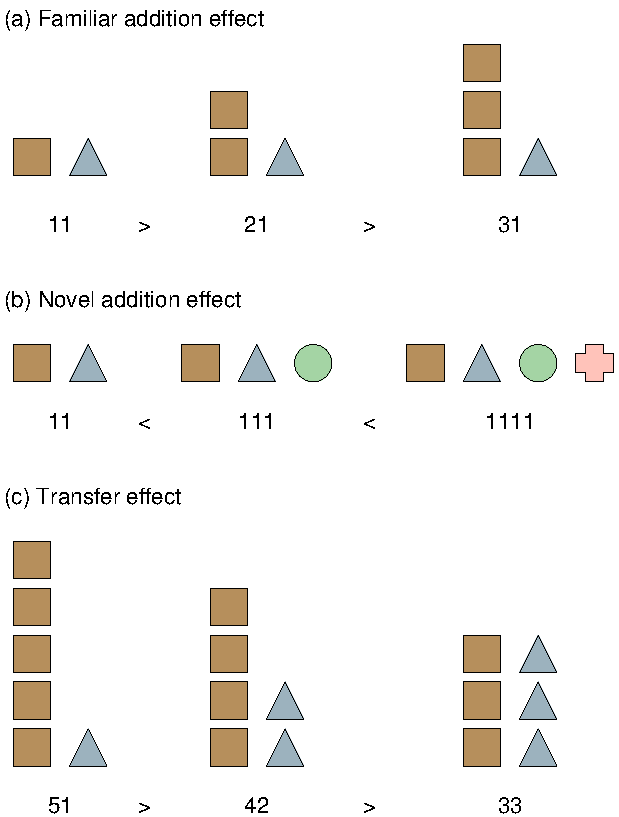
\includegraphics[scale=0.7]{introfig2-eps-converted-to.pdf}
\caption{Frequency distributions based on chocolates sampled from three boxes. For example, distribution 31 includes three chocolates from one category (brown squares) and one chocolate from a different category (blue triangle). The inequalities shown below each panel represent predictions about the probability that the next object sampled will belong to a novel category.
(a) The familiar addition effect. Observing a new exemplar that belongs to a familiar category decreases the probability that the next object sampled will belong to a novel category. (b) The novel addition effect. Observing a new exemplar that belongs to a novel category increases the probability that the next object sampled will belong to a novel category. (c) The transfer effect. Transferring an object from a high-frequency category to a low-frequency category decreases the probability that the next object sampled will belong to a novel category.}
\label{fig:intro}
\end{center}
\end{figure}

Here we consider six distinct Bayesian models that build upon Anderson's rational model. The key difference between these models is in how they exploit the frequency distribution over categories.  The intuitive relevance of distributional information is highlighted in Figure~\ref{fig:intro}, which depicts several examples in which a series of chocolates are sampled from boxes. In the first example (Figure~\ref{fig:intro}a) the learner initially observes two different kinds of chocolates (the \dist{11} case), and as more chocolates appear they all belong to one of the initial two categories. This sequence of distributions \dist{11}\goesto\dist{21}\goesto\dist{31} is an example of what we will call the {\it familiar addition} effect. Intuition suggests that as this sequence continues, we should become more convinced that there are only two types of chocolate and that no new categories will be encountered: that is, adding new observations to old categories should decrease the learner's expectation that new categories will appear.

In contrast, consider the sequence depicted in Figure~\ref{fig:intro}b, in which each new observation belongs to a novel category, producing the sequence \dist{11}\goesto\dist{111}\goesto\dist{1111}. This sequence is an example of a {\it novel addition} effect, and in this case intuition suggests that each observation raises the probability that the next object observed will belong to a novel category. The familiar and novel addition effects both seem very intuitive, but existing category learning models do not capture them both. For instance,  Anderson's rational model captures the familiar addition effect but not the novel addition effect. In particular, this model makes the unintuitive prediction that distributions \dist{31} and \dist{1111} provide equal support for the hypothesis that the next sample will belong to a novel category.

As a third -- and less obvious -- example, Figure~\ref{fig:intro}c depicts a sequence \dist{51}\goesto\dist{42}\goesto{33} illustrating the {\it transfer effect} in which the numbers of exemplars and categories both remain constant but the distribution of exemplars across the categories does not. As exemplars are shifted ``down'' from high frequency categories to low frequency ones (from left to right) the frequency distribution becomes less skewed and more balanced. Our intuitions about 1c are less strong than our intuitions about 1a and 1b, but encountering a novel category seems more likely given the skewed distribution (\dist{51}) than given the balanced distribution (\dist{33}). A plausible explanation for this inference is that skewed distributions provide more support for the idea that there are low-frequency categories that have not yet been observed.


As we will see, people are sensitive to all three effects in Figure 1, but many
computational models are not. We demonstrate that two of the six Bayesian
models that we consider are able to capture all of these effects, but all other models evaluated in this paper fail to capture at least one of the effects.

The structure of the paper is as follows. In the next section we discuss a set of intuitively reasonable axioms that give rise to the six Bayesian models.
We then present four experiments that probe the extent to which these models capture qualitative and quantitative aspects of people's inferences about novel categories.  Experiments 1 and 2 explore how people respond to different frequency distributions, and include cases similar to those shown in Figure~\ref{fig:intro}.  Both experiments use a paradigm in which participants predict the probability that the next object encountered will belong to a novel category. Experiments 3 and 4 use  a more traditional paradigm in which participants are shown a new object and can either assign it to an old category or indicate that it belongs to a novel category. We vary the extent to which the new object is similar to previously encountered objects, and find that people's judgments are influenced both by similarity and distributional information. Following the experiments, we discuss the extent to which alternative approaches from the psychological and statistical literatures can account for our data, and compare the performance of the Bayesian models to eleven heuristic models.

\section{A Bayesian framework for novelty detection}

In order to develop specific probabilistic models for the detection of novel categories, it is useful to situate the problem within the broader problem of categorization. Our formulation of this problem is most naturally applicable to supervised settings in which the learner uses explicit feedback to learn categories, but the problem of novelty detection is more general. As discussed later in the paper the novelty detection problem is closely connected to unsupervised categorization, and our probabilistic approach can easily be extended to semi-supervised settings \cite<e.g.,>{gibson_human_2013,VongPerforsNavarro2016} or settings involving cross-classified stimuli \cite<e.g.,>{shafto_probabilistic_2011,ross_food_1999}.

\subsection{Assigning new objects to old categories}

A probabilistic account of supervised classification can be constructed as follows. Suppose that the learner has encountered $N$ labelled objects. We use $x_i$ to denote the set of features associated with the $i$-th object, and use $l_i$ to refer to the category label for that object. Across all $N$ objects, then, the information available to the learner consists of all the featural information $\bm{x}_{1:N}=(x_1, x_2, \ldots, x_N)$ and all of the category labels $\bm{l}_{1:N}=(l_1,l_2,\ldots,l_N)$. Taken together, $\bm{x}_{1:N}$ and $\bm{l}_{1:N}$ capture the relevant background knowledge that the learner can use  when seeking to classify a newly observed object.

If the problem of categorization is formulated in this way, what should a Bayesian learner infer about the label of a novel object? Consider first the case in which the learner knows that there are exactly $K$ possible category labels. Bayes' rule indicates that the probability that the new object belongs to category $k$ is
\begin{equation}
\begin{array}{l}
P(l_{N+1} = k \given x_{N+1}, \bm{x}_{1:N}, \bm{l}_{1:N})
 \\ \ \ \ \ \ \ \ \propto \ \
P(x_{N+1} \given l_{N+1} = k, \bm{x}_{1:N}, \bm{l}_{1:N}) \ P(l_{N+1} = k \given \bm{x}_{1:N}, \bm{l}_{1:N})
\end{array}
\label{basicbayes}
\end{equation}
where the normalizing term is found by summing over all $K$ possible choices for the category label. The first term in this expression is the {\it likelihood function} that describes the learner's beliefs about the probability that an object would have features $\bm{x}_{N+1}$ if it were sampled from the $k$-th category. Anderson \citeyear{anderson_adaptive_1991} describes how this term can be formulated for settings in which objects have discrete features, and settings in which these features are continuous. Its role within the model is to serve as a measure of the extent to which the new object is consistent with a particular category, and we discuss its connection to the theory of novelty detection later in the paper.

The second term in Equation~\ref{basicbayes} describes the learner's {\it prior} over the category labels, and its psychological role in the model is to serve as the learner's estimate of the category base rates. If a novel object has features that are equally consistent with two categories, then a Bayesian reasoner will guess that the new object belongs to the category with the higher base rate. Consistent with this interpretation as a measure of subjective base rate, the prior distribution over the next label $l_{N+1}$ is assumed to depend on the labels $\bm{l}$ of the previously observed stimuli but not upon their features $\bm{x}_{1:N}$. If this assumption holds, we can drop this term from the prior and express the learner's beliefs about the category labels as $P(l_{N+1} = k \given \bm{l}_{1:n})$. Furthermore, it is traditional to assume that the observations are {\it exchangeable}, in which case the order in which the labels appear carries no information \cite<but see, e.g.,>{navarro_learning_2013}. Under the assumption of exchangeability, all of the relevant background knowledge is carried by the {\it frequency table}. If we let $n_k$ denote the number of objects known to belong to category $k$, and let $\bm{n} = (n_1, n_2, \ldots, n_K)$ denote the frequency table for all $K$ categories, the prior probability of category $k$ in Equation~\ref{basicbayes} simplifies to
\begin{equation}
P(l_{N+1} = k \given \bm{x}_{1:N}, \bm{l}_{1:N}) = P(l_{N+1} = k \given \bm{n}).
\end{equation}

Given a frequency table $\bm{n}$, what should the learner believe about the
category label of the next object?  A naive approach is to rely on the
empirical base rates and to treat the probability that the next
exemplar belongs to the $k$-th category as equal to the proportion of
existing exemplars that belong to that category, yielding the model
\begin{equation}
P(l_{N+1} = k \given \bm{n}) = \frac{ n_k }{ N }.
\label{empirical}
\end{equation}
This estimate of category frequencies arises in some uses of naive Bayes classifiers \cite<e.g.,>[section 20.2]{russell_artificial_2003} and -- as we discuss later in the paper -- is implicitly adopted by some non-Bayesian models such as the generalized context model \cite<GCM:>{nosofsky_attention_1986}. Despite its intuitive appeal this approach becomes incoherent when we consider the possibility of never-before-seen categories. Under this model, the prior probability that the next observation belongs to a {\it new} category is estimated to be zero, so a Bayesian reasoner who uses the prior in Equation~\ref{basicbayes} is unable to entertain the possibility of novel categories. The only categories that this learner can acquire are categories that are already known to exist! We therefore need some alternative way of characterizing the way in which a frequency table shapes expectations about the category of the next object to be observed.

\subsection{One solution to the novelty detection problem}

Anderson's \citeyear{anderson_adaptive_1991} rational model of categorization (RMC) provides one possible solution to the problem. When presenting his original rational analysis, Anderson suggested that the learner assumes that there is some fixed ``coupling probability'' that any two objects belong to the same category, and from that assumption went on to derive the probability that the next object belongs to a novel category. As discussed by \citeA{sanborn_rational_2010}, it turns out that Anderson's analysis from first principles induces a prior that is formally equivalent to a well-known model in Bayesian statistics (the {\it Chinese restaurant process}; CRP). According to the CRP the prior probability of an old category is proportional to its observed frequency $n_k$ (as per the naive model in Equation~\ref{empirical}), but the CRP also assigns some strength $\theta$ to the possibility that the next observation will come from a new category. Thus, under the CRP prior the probability that the next object comes from the $k$-th old category is
\begin{equation}
\label{eq:crpold}
P(l_{N+1} = k \given \bm{n}) = \frac{n_k}{\theta + N}
\end{equation}
and the prior probability that the next object will be an exemplar from a hitherto unobserved category is given by
\begin{equation}
P(l_{N+1} = \mbox{new} \given \bm{n}) = \frac{\theta}{\theta + N}
\label{eq:crpnew}
\end{equation}
The strength parameter $\theta$ is directly related to Anderson's original coupling probability \cite{sanborn_rational_2010}, and is a free parameter in the RMC that controls the probability
that new categories will be encountered.

Perhaps because of the success of Anderson's model \cite{anderson_adaptive_1991,griffiths_unifying_2007,sanborn_rational_2010}, the CRP model has served as the standard solution to the problem of novelty detection not only in the original RMC, but across the many extensions and elaborations of the model
\cite<e.g.>{shafto_probabilistic_2011,kemp_learning_2007,perfors_learning_2009}.
It is also used more generally in the literature on nonparametric Bayesian statistics \cite<see e.g.,>{gershman_tutorial_2012,navarro_modeling_2006}. However, although the CRP model is widely adopted as the solution to the problem of novelty detection, it has rarely been directly investigated (see \citeA{austerweil_testing_2014} for one exception). There are reasons to believe that it may not adequately capture people's expectations about novel categories.
The CRP predicts, for example,
that the probability of encountering a novel category depends only on the
strength parameter $\theta$ and the number $N$ of objects already observed.
This is a strong empirical prediction that may not adequately capture people's intuitions about when to expect novel categories.

\subsection{Deriving a more general model from qualitative desiderata}

 Arguably, much of the appeal of the CRP model stems from the fact that Anderson's analysis makes the psychological assumptions of the model explicit. The model described by Equations~\ref{eq:crpold} and \ref{eq:crpnew} is simple, and the strength parameter $\theta$ is straightforward to interpret as a pseudo-sample size: the possibility of a new category is assigned prior weight as if it were an old category with an observed sample size of $\theta$. It is possible, however, that other assumptions -- and hence other priors -- might be better matched to human cognition. Rather than attempt to specify {\it a priori} what set of assumptions might be ``optimal'' for human cognition, we consider a family of plausible models and seek to test their predictions empirically without making strong claims as to which (if any) of these models constitutes a normative standard for categorization \cite<e.g.>{TauberNavarroPerforsSteyvers}.

An elegant way to develop alternative approaches is to formulate axioms that specify psychologically meaningful constraints on the beliefs that a learner might have about categories. Consider the categorization problem as it appears to a learner who observes a sequence of objects and their corresponding labels. What qualitatively sensible constraints might a learner impose? Zabell \citeyear{zabell_carnap_2011} suggests the following desiderata:
\bigskip
\begin{enumerate}[label={(\arabic*)}]
\item Anything is possible: the learner does not know ahead of time what categories exist, and does not rule out any sequence of labels {\it a priori}. Formally this axiom requires that every sequence of category labels has positive probability. \smallskip
\item The probability of every old category depends only on its own observed frequency. That is, the probability that the next object will belong to a previously observed category depends on the observed base rate of that category, but not on the base rates of other categories. Formally, this axiom states that the probability of old category $k$ depends only on the number of objects $n_k$ observed to belong to category $k$ and the total sample size $N$.\smallskip
\item The probability of a new category depends on how frequently new categories have appeared in the past. More precisely, this axiom claims that the probability that the next observation belongs to a hitherto unobserved category is a function only of the number of observed categories $K$ and the sample size $N$.
\end{enumerate} \bigskip
If we further assume that there are at least two categories,\footnote{In fact Zabell does not assume that there are least two categories, and in this case the family of distributions is rather more complicated and is characterized by three parameters. However, one of these parameters is no longer relevant if the learner knows that there are at least two categories. Given that most realistic situations involve scenarios where at least two categories are known to exist, we use the restricted two-parameter version described in the text.} Zabell shows that these three axioms give rise to a very simple family of possible prior distributions that is characterized by two parameters,
$\theta$ and $\alpha$. For distributions in this family, the probability that the next observation belongs to the $k$-th existing category is
\begin{equation}
\label{eq:gcrpold}
P(l_{N+1} = k \given \bm{n}) = \frac{n_k - \alpha}{\theta + N}
\end{equation}
and the probability that it belongs to a novel category is
\begin{equation}
\label{eq:gcrpnew}
P(l_{N+1} = \mbox{new} \given \bm{n}) = \frac{\theta + K\alpha}{\theta + N}
\end{equation}
where $0 \leq \alpha \leq 1$ and $\theta + \alpha > 0$. These equations define a stochastic process that is known as the {\it generalized Chinese restaurant process} \cite<G-CRP: see>{ishwaran_generalized_2003}, and is closely related to the Pitman-Yor process \protect\cite{pitman_two-parameter_1997}.\footnote{Strictly speaking the G-CRP is a stochastic process that generates exchangeable random partitions whereas the Pitman-Yor process (PYP) is usually taken to define a stochastic process that generates probability distributions. However, the two are closely connected: every distribution sampled from the PYP is associated with a partition that assigns each observation to a cluster, and the partitions associated with a PYP-generated distribution follow a G-CRP. Given the slightly inconsistent way in which the PYP is defined, we have chosen to adopt the terminology from \citeA{ishwaran_generalized_2003} in which G-CRP is used to describe the process that generates partitions, and the PYP is defined more narrowly to refer to the closely related process that generates probability distributions.} The G-CRP has been used by \citeA{goldwater_producing_2011} to develop
statistical models of language, and has found multiple other applications
in the statistics and computer science literatures. As yet, it has
found few applications in the psychological literature, but it has
considerable potential as a theory of novelty detection.

\begin{table}
\caption{Three Bayesian models for the novelty detection problem that can be derived via Zabell's axiomatic formulation of the problem (CRP, TTR, G-CRP) and their three hierarchical counterparts (H-CRP, H-TTR, HG-CRP).}
\label{modellist}
\begin{tabular}{l|ll}
& \multicolumn{2}{|c}{Parameter} \\
Model  &  Strength, $\theta$ &  Discount, $\alpha$ \\ \hline
Chinese restaurant process (CRP) & Fixed & 0 \\
Types-tokens ratio (TTR) & 0 & Fixed \\
Generalized Chinese restaurant process (G-CRP) & Fixed & Fixed \\
Hierarchical Chinese restaurant process (H-CRP) & Learned & 0 \\
Hierarchical types-tokens ratio (H-TTR) & 0 & Learned \\
Hierarchical generalized Chinese restaurant process (HG-CRP) & Learned &  Learned
\end{tabular}
\end{table}


Viewed as a model of novelty detection, the G-CRP model offers an intriguing extension to the more traditional CRP model. In this account, the probability that the next observation belongs to a novel category is the sum of two components. The first of these is the $\frac{\theta}{\theta+N}$ term from the more familiar CRP model: the learner assigns some base level of {\it strength} $\theta$ to the possibility that a new category will appear, and this $\theta$ parameter can be viewed as a pseudo-sample size associated with unobserved categories. The second term is $\frac{K \alpha}{\theta+N}$, which depends on the number of categories $K$ that the learner has encountered thus far. This term ensures that the more often that the learner actually encounters a new category (which, by definition, must have occurred $K$ times), the more likely it is that even more new categories will subsequently appear. This idea has an intuitive appeal, and the extent to which the model is sensitive to it is governed by the {\it discount} parameter $\alpha$.

The role of the discount parameter can be described in the following way. In the CRP model, every category has some strength, and the probability of that category is proportional to its strength. Every time a new observation is assigned to an existing category the strength increases by 1. When a new category is detected, however, there are two different things the learner might wish to strengthen: the specific new category (which is now known to exist), {\it and} the background belief that new categories will continue to appear. In the G-CRP model, the strength ``associated'' with the most recent observation is split between these two possibilities. The newly discovered category is only given a strength of $1-\alpha$ (Equation~\protect\ref{eq:gcrpold}) and the remaining strength $\alpha$ is siphoned off and used to give additional strength to the possibility that the next observation will belong to yet another new category (Equation~\protect\ref{eq:gcrpnew}).

In light of this discussion, Zabell's three axioms give rise to three distinct probabilistic models for the novelty detection problem, listed at the top of Table~\ref{modellist}. The CRP model assumes that people assign a fixed strength $\theta$ to new categories, whereas the G-CRP model augments this with a discounting process governed by $\alpha$ that strengthens the prior probability of new categories every time a new category is observed. A third possibility is that people {\it only} rely on the discounting process. That is, if we set $\theta = 0$ then the prior probability of a new category is given by $\frac{\alpha K}{N}$. Given that $\frac{K}{N}$ defines the proportion of observations (tokens) that introduced a new category (types), we refer to this approach as the {\it types-tokens ratio} model (TTR).
 This model is closely related to a stochastic process known as the normalized stable process that has been explored in the statistics \cite{kingman_random_1975} and machine learning \cite{wood2009stochastic} literatures. Thus all three models have some intuitive justification, and any one might make sense as a prior in a Bayesian categorization model.




\subsection{Learning the parameters of the prior distribution}

The qualitative desiderata introduced by Zabell produce an elegant theory that uses an observed frequency table $\bm{n}$ to estimate the probability that the next observation will represent a new category. However, these estimates are dependent on two unknown parameters, the strength $\theta$ and discount rate $\alpha$. How should these values be set? One possibility is that these parameters represent {\it fixed} biases that the learner brings to the categorization problem. According to this view, $\theta$ and $\alpha$ should be treated as model parameters: that is, quantities that the researcher needs to estimate from people's behavior. This is the standard way in which researchers have interpreted these parameters in the past. For instance, in the original applications of the RMC, Anderson \citeyear{anderson_adaptive_1991} used a fixed strength parameter of approximately $\theta=2.3$, suggesting that people assign roughly the same prior weight to never-observed categories that they would give to an actually-observed category with two known exemplars.\footnote{Anderson actually set his coupling parameter to $c=.3$. As noted by \citeA{sanborn_rational_2010}, the relationship between the two is $\theta=(1-c)/c$, yielding $\theta \approx 2.3$.}

An alternative perspective is offered by considering the novelty detection problem from the perspective of learners who endorse Zabell's axioms but have little or no other knowledge beyond the desire to satisfy these desiderata. These learners would agree that Equations~\ref{eq:gcrpold} and \ref{eq:gcrpnew} provide a good description of the ``true'' generative process that gives rise to the available observations, but would have no compelling reason to make strong assumptions about the true values of $\alpha$ or $\theta$. From this perspective, these parameters are quantities that the learners must learn from experience. If the learners are Bayesian, they would place a prior over $\alpha$ and $\theta$, and update this prior as the observations arrive. This perspective gives rise to the hierarchical Bayesian versions of the three models listed in the lower half of Table~\ref{modellist}, in which a learner uses the frequency table $\bm{n}$ not only to estimate the probability of a new category, but also to learn the statistical properties of the stochastic process that generates their observations. To formalize this idea we consider the most general model, the {\it hierarchical generalized Chinese restaurant process} (HG-CRP), since the other two models are special cases.

\begin{figure}
\begin{center}
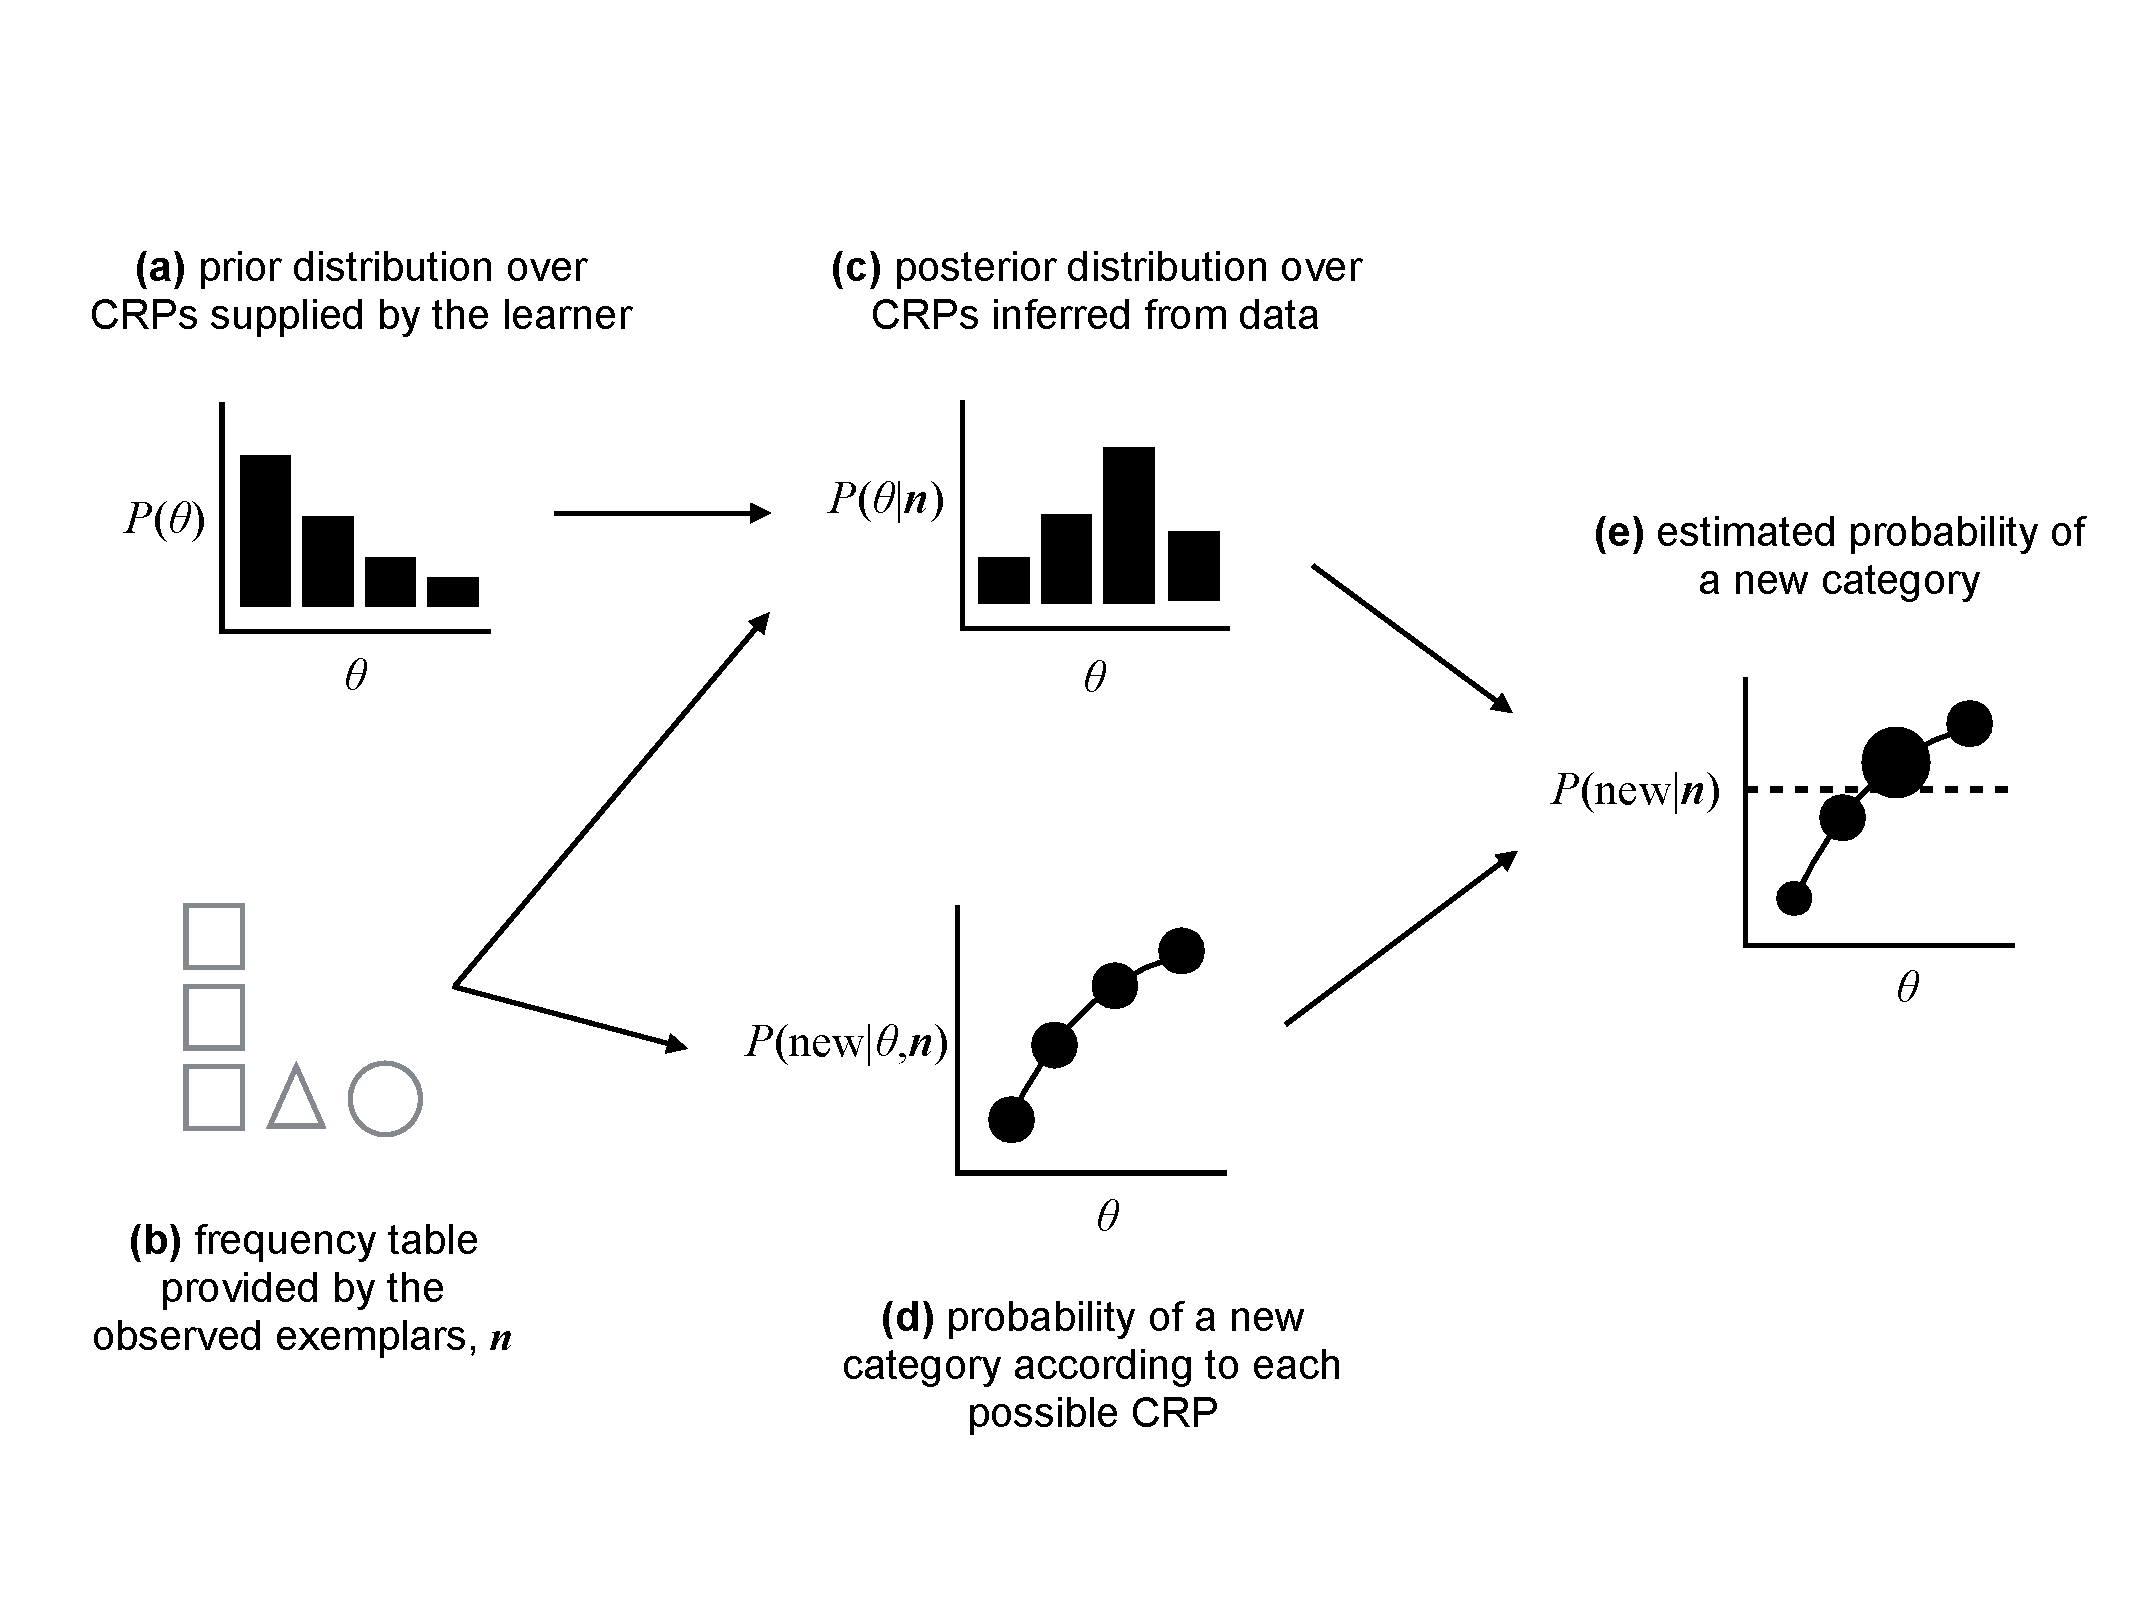
\includegraphics[scale=0.4]{hcrp_schematic.pdf}
\caption{A schematic illustration of the H-CRP model. The learner supplies a prior distribution over the strength parameter $\theta$ (panel a), and then observes a frequency table $\bm{n}$ (panel b). From this the learner infers the posterior distribution $\theta|\bm{n}$ (panel c). Given that every CRP (i.e., each value of $\theta$) produces a specific prediction about the probability of a new category given the observed frequency table (panel d), the learner can construct an estimate of the probability of a new category (panel e) by taking a weighted average of the prediction of each possible CRP (i.e., the dashed line). In panel e, the size of the points is analogous to the height of the bars in panel c, illustrating the fact that the estimate produced by the model is a posterior-weighted average of the individual CRPs. The H-TTR and HG-CRP models are constructed in an analogous fashion.}
\label{schematic}
\end{center}
\end{figure}

Suppose that a learner approaches the novelty detection problem with a prior $P(\theta,\alpha)$ that expresses their uncertainty, and seeks to infer those parameters from the observed frequency table $\bm{n}$. In this instance, Bayes' rule gives
\begin{equation}
\label{parameterlearning}
P(\theta,\alpha | \bm{n}) \propto P(\bm{n} | \theta,\alpha) P(\theta,\alpha)
\end{equation}
where the probability of the frequency table $P(\bm{n} | \theta,\alpha)$ can be constructed by sequentially applying Equations~\ref{eq:gcrpold} and~\ref{eq:gcrpnew} as each new observation arises. Given a specific frequency table $\bm{n}$ and the inferred distribution over the parameters $P(\theta,\alpha | \bm{n})$, the probability that the next observation represents a hitherto unseen category is estimated by taking a weighted average of the predictions of every possible G-CRP model. More precisely, the learner constructs the marginal probability of a new label by integrating out $\theta$ and $\alpha$,
\begin{equation}
\label{eq:hgcrpnew}
P(\mbox{new} \given \bm{n}) = \int_0^1 \!\! \int_{-\alpha}^\infty \ \frac{\theta + K\alpha}{\theta + N} \ P(\theta, \alpha \given \bm{n}) \ d\theta \ d\alpha
\end{equation}
Equation~\ref{eq:hgcrpnew} describes the predictions of the HG-CRP model, corresponding to a Bayesian reasoner who uses the observed data to infer the strength $\theta$ and discount $\alpha$ parameters. However, if the Bayesian reasoner started with one of the two restricted models (i.e., CRP and TTR) rather than the full G-CRP model implied by Zabell's axioms, then one of other two hierarchical models (i.e., H-CRP and H-TTR) would result. The predictions from these models are constructed by analogy to Equation~\ref{eq:hgcrpnew}, with one of the two parameters fixed at 0.

In order to construct a specific model that can be applied to human categorization judgments, it remains to specify the prior distributions that the learner brings to the task. In our applications we assume that the learner has independent priors over the two parameters, implying that $P(\theta,\alpha)=P(\theta)P(\alpha)$. For the strength parameter $\theta$ we use a generalized Pareto distribution\footnote{Specifically, a generalized Pareto with location parameter 0.}, and for the discount parameter $\alpha$ we use a beta distribution,
\begin{eqnarray}
P(\theta) &=& \frac{1}{\sigma}\left(1+\frac{\xi\theta}{\sigma}\right)^{-(1+1/\xi)}\\
P(\alpha) &\propto& \alpha^{\beta_1 - 1} (1-\alpha)^{\beta_2 -1}
\end{eqnarray}
where $P(\theta)$ is defined in terms of a shape parameter $\xi$ and a scale parameter $\sigma$, and $P(\alpha)$ is defined in terms of two pseudo-count parameters $\beta_1$ and $\beta_2$.

Formal details aside, the important characteristic of all three hierarchical models is that the learner uses the observed frequency table $\bm{n}$ to {\it infer} what {\it kind} of generative model underpins the distribution of category labels. This approach is illustrated schematically in Figure~\ref{schematic} using the H-CRP model as an example. Similar hierarchical approaches have previously been used to explore how people form general expectations about the features associated with categories (the likelihood in Equation~\ref{basicbayes}), allowing them to make sensible predictions about entirely novel categories \cite<e.g.,>{kemp_learning_2007,perfors_learning_2009,PerforsNavarroTenenbaumSUBMITTED,navarro_learning_2010}. However, we know of no psychological work using the RMC or related models that allows the strength parameter $\theta$ to be learned, and almost no work that considers the discount parameter $\alpha$ at all.


\subsection{Overview of the experiments}

The qualitative principles outlined by Zabell give rise to three different models (CRP, TTR, G-CRP) that a Bayesian reasoner might use to specify a prior for the novelty detection problem. When we extend Zabell's model to accommodate the idea that the learner infers which specific CRP/TTR/G-CRP prior to apply, we obtain three more models (H-CRP, H-TTR, HG-CRP) that might underpin human categorization. Slotting these priors into Equation~\ref{basicbayes} produces six different Bayesian models of categorization, each of which is a variation on Anderson's (1991) rational model. In order to evaluate these six models we present a series of four experiments that explore human intuitions about the novelty detection problem. To keep our presentation as simple as possible, our initial evaluation focuses on these six Bayesian models. Later in the paper we extend this evaluation by describing several non-Bayesian models and considering the extent to which they account for our experimental data. To foreshadow our conclusions, only some of the Bayesian models (and none of the non-Bayesian models) provide an adequate account of human behavior. Beginning with the Bayesian models therefore allows us to illustrate what principles a successful model of human novelty detection must satisfy.

The structure of the experimental work is as follows. In the first experiment, we focus on the standard CRP model and show that it systematically fails to capture human judgments, illustrating the need to move beyond Anderson's original formulation of the problem. The second experiment is designed to discriminate between the six models, and finds evidence that the discount parameter $\alpha$ and the hierarchical learning mechanism are both necessary. We show that the superior performance of the hierarchical models (especially the four-parameter HG-CRP model) is not an artifact of model flexibility, and that the model is highly constrained in terms of the qualitative patterns of performance that it can produce.  The third experiment presents evidence from a standard categorization task in which object similarity information is made available to participants, and the fourth experiment adapts this standard design to more cleanly separate frequency and similarity information. In both experiments we find that frequency information continues to play an important role even when similarity information is available, and that the basic CRP model continues to make incorrect predictions that are only remedied by adopting a hierarchical approach.


\section{Experiment 1}

Our initial exploration takes a systematic approach, and considers all possible frequency tables constructed from six or fewer exemplars. By comparing people's intuitions about different frequency tables we can test whether the assumptions of the simple CRP model are correct, or whether more elaborate models are required to explain people's expectations about undiscovered categories.


\subsection{Method}

\subsubsection{Participants} The study was completed by 200 workers on Amazon Mechanical Turk, who were paid US\$1.50 for their time (approximately 10 minutes). 176 participants were located in the United States, and 24 in India. 114 self identified as male, 84 as female, 1 as other.

\subsubsection{Materials \& Procedure}

The goal of the experiment was to present people with frequency tables that divided a set of exemplars into categories, and to measure people's beliefs about the probability that the next object would come from a hitherto unobserved category. To that end, the cover story presented people with the following text:

\begin{quote}{\it
Scientists interested in studying insect biology stake out square meter blocks, and record the number of insects of different kinds that they see. In this task you'll be shown the results of 29 different ``insect trap'' experiments, taken from different parts of the world. No two sites are alike, and different species are found at each location.

For all 29 sites, you'll be shown a list of the insects that have been observed so far. Your task is to judge the probability that the next insect to be observed at that location will belong to a new species, or one of the previous ones.}
\end{quote}
Participants were told that species were identified solely in terms of an arbitrary identification code such as ``GX12'', and that the various sites were unrelated and would involve completely different insects. On each trial they were shown a stimulus display that listed the insects captured so far. For example, the following display
\begin{verbatim}
                                   GX12
                                   GX12
                              NS81 GX12 BL56
\end{verbatim}
indicates that the trap has captured three GX12 insects, one NS81 and one BL56. The assignment of species code and the ordering of categories was randomized, but always preserved the ``barplot-style'' display shown above. Participants were asked to judge the probability that the next insect captured by the trap would belong to a new species (i.e., a species other than GX12, NS81, or BL56). Responses were made using a slider bar, and participants were allowed to familiarize themselves with the interface before proceeding with the task. They also had to answer three instruction-check questions correctly before the task began.

The 29 within-subject experimental conditions differed in terms of the category frequencies. Using notation from Figure~\ref{fig:intro}, the example given above depicts a \dist{311} frequency table, since the learner has seen three exemplars from one category (GX12) and one exemplar each from two other categories (NS81 and BL56). The experiment presented all 29 possible frequency distributions defined over six or fewer exemplars. These distributions are listed in Table~\ref{tab:exp1}.


\begin{table}
\caption{The 29 distributions used in Experiment 1 correspond to the set of all possible frequency tables defined over six or fewer exemplars. The listing below displays these 29 conditions as a function of the number of exemplars $N$ and the number of categories $K$ over which they are distributed.\vspace*{6pt}}
\label{tab:exp1}
\footnotesize
\begin{tabular}{l|r|rrr|rrr|rr|r|r}
               & $K=1$  & \multicolumn{3}{c|}{$K=2$} & \multicolumn{3}{c|}{$K=3$}
               & \multicolumn{2}{c|}{$K=4$ } & $K=5$  & $K=6$
               \\ \hline
$N=1$  & \dist{1} &&&&&&&&&  \\
$N=2$  & \dist{2} & \dist{11} &&&&&&&&  \\
$N=3$  & \dist{3} & \dist{21} &&& \dist{111} &&&&& \\
$N=4$  & \dist{4} & \dist{31} & \dist{22} && \dist{211} & \dist{1111} &&&& \\
$N=5$  & \dist{5} & \dist{41} & \dist{32} && \dist{311} & \dist{221} && \dist{2111} && \dist{11111} \\
$N=6$  & \dist{6} & \dist{51} & \dist{42} & \dist{33} & \dist{411} & \dist{321} & \dist{222} & \dist{3111} & \dist{2211} & \dist{21111} & \dist{111111}
\end{tabular}
\end{table}


\subsubsection{Exclusions} Participant responses fell into one of three distinct groups, identified by clustering analysis. 163 participants (82\%) produced responses that were consistently positively correlated with one another across all 29 conditions, suggesting that these participants were using qualitatively similar strategies.  Visual inspection of the responses hinted that 5 of these 163 participants had been misclassified by the algorithm, leaving 158 participants (79\%) whose responses are all in strong agreement. Of the remaining participants, 16 (8\%) were consistently negatively correlated with the majority, suggesting that they unintentionally reversed the response scale. The remaining 20 participants (10\%) gave answers that were uncorrelated with any other participant. Across these participants the average response was very close to 50\% for all conditions, suggesting that these participants gave random responses. We present data from the majority group only, but note that this has essentially no effect on the results: the majority group is so consistent and the minority response patterns are so rare and dissimilar that including them has no effect on the averages other than to create a slight regression to the mean.

\subsection{Results}



\begin{figure}[p]
\begin{center}
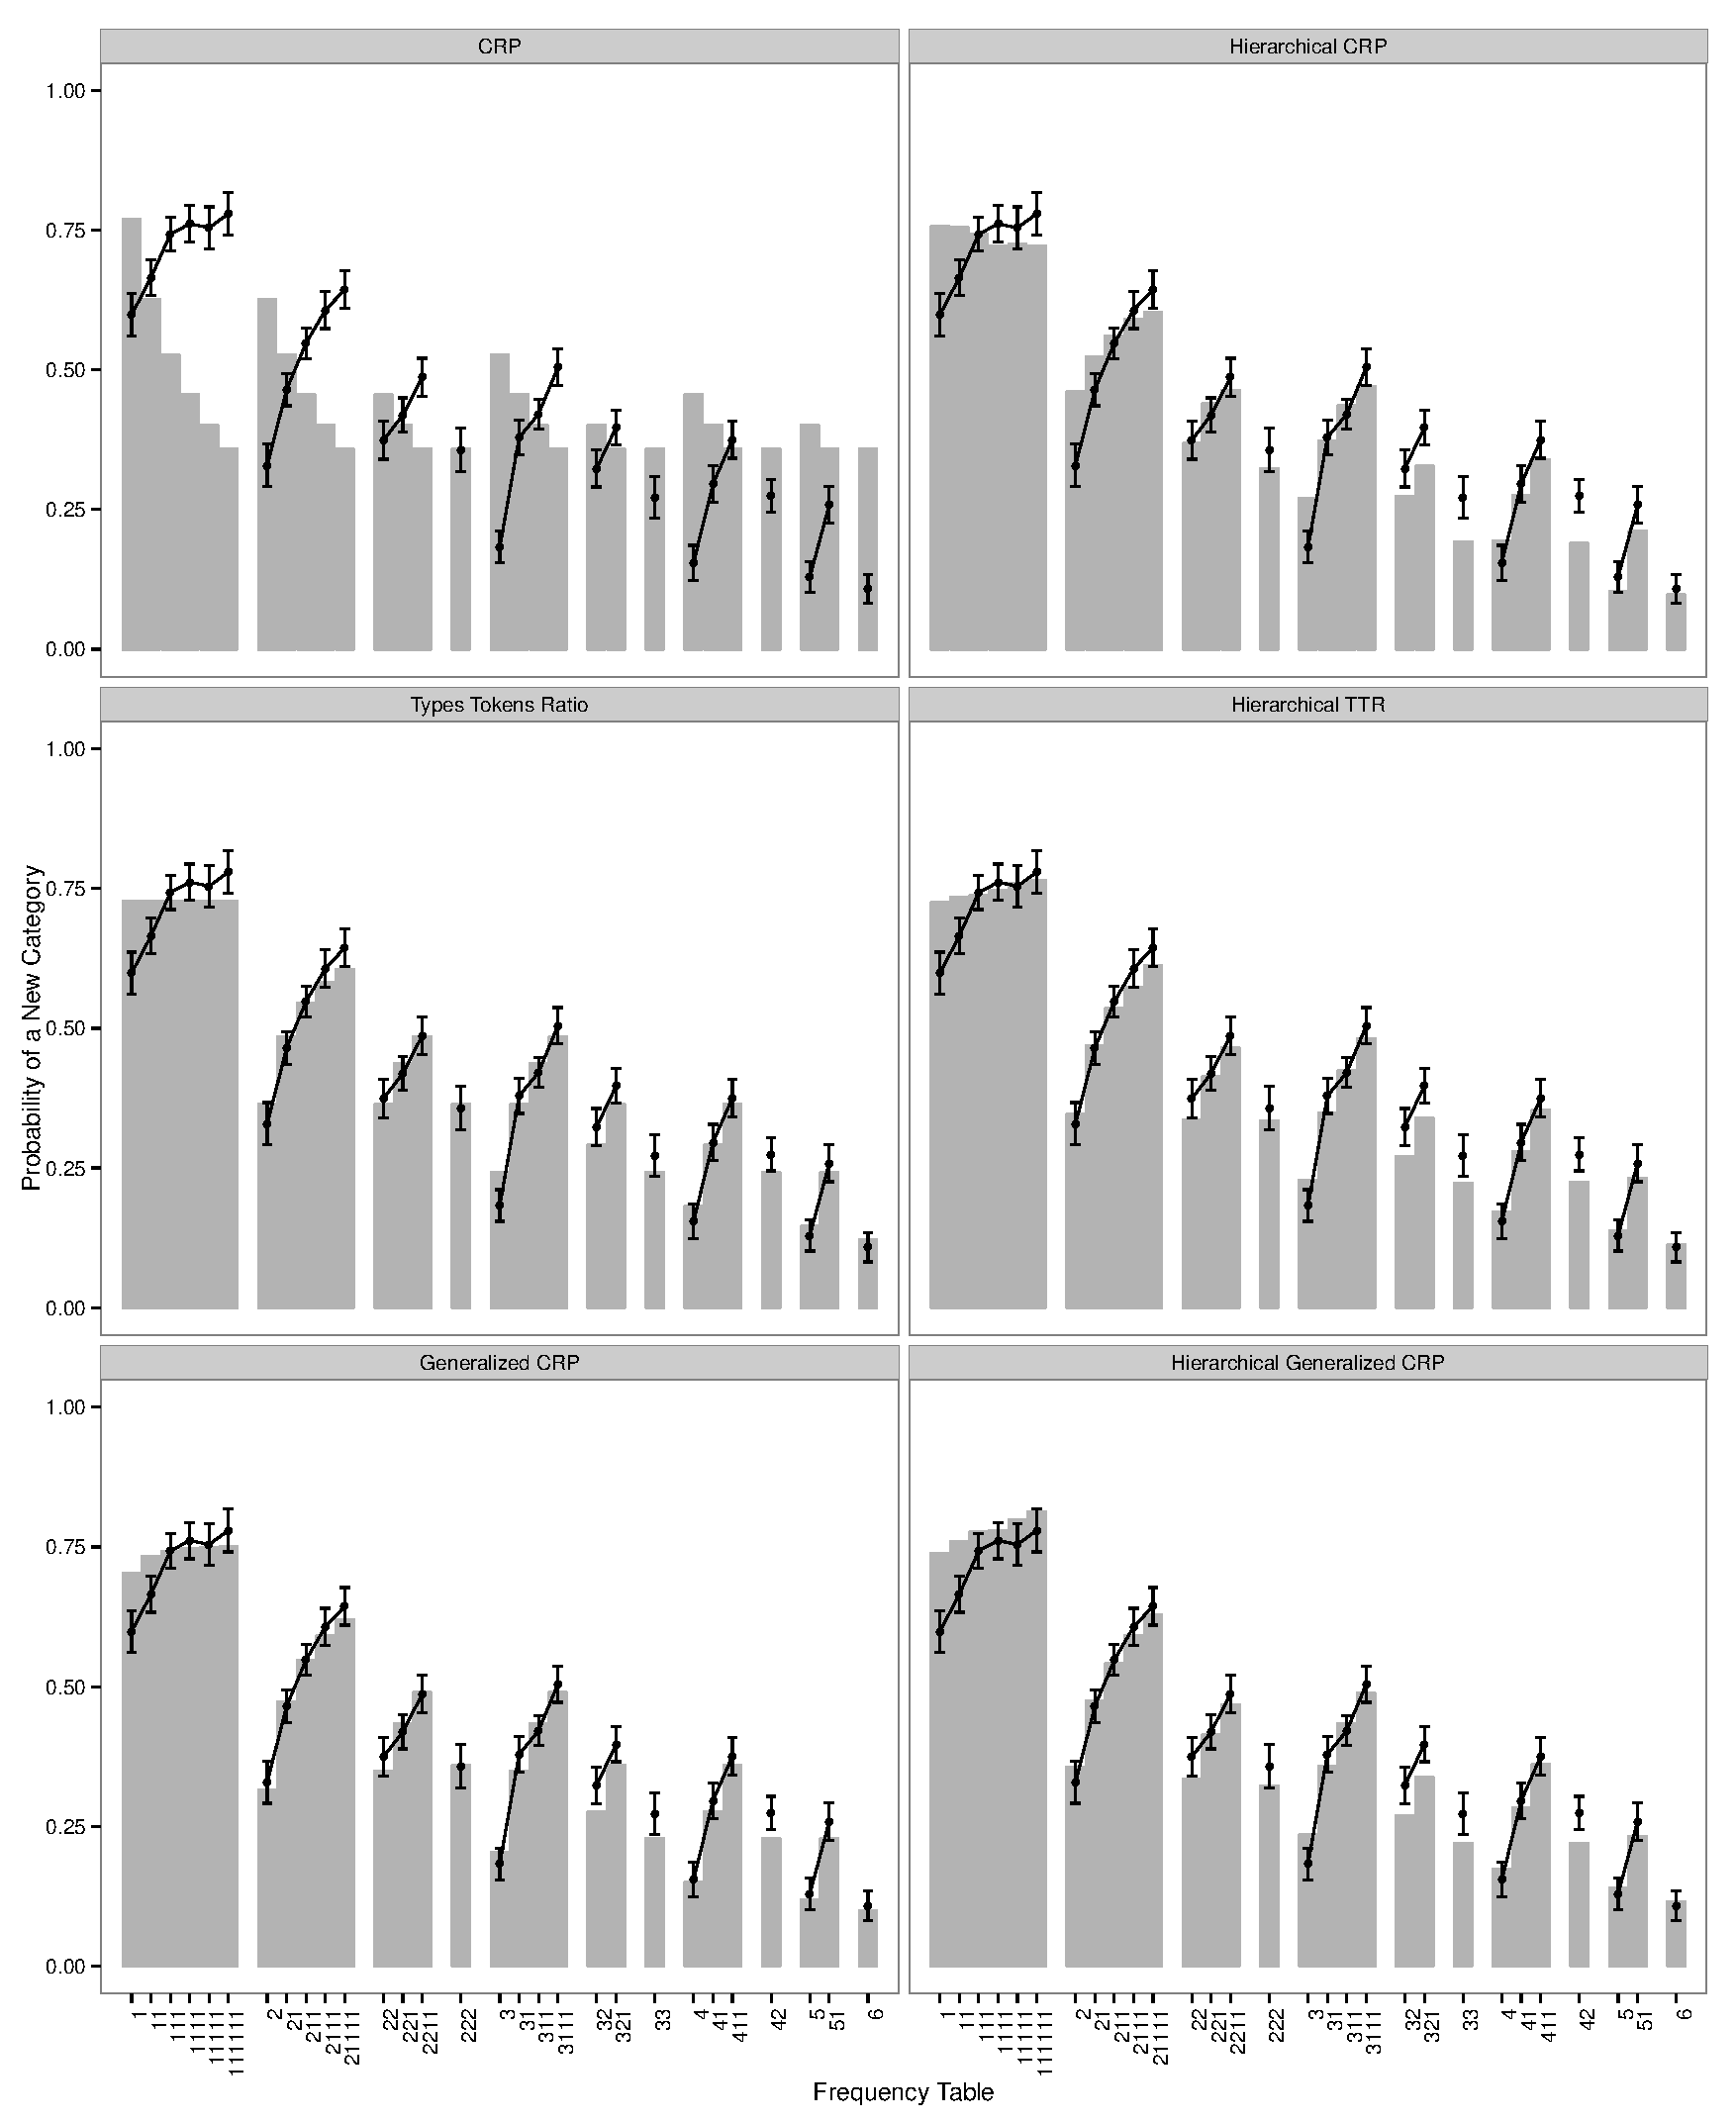
\includegraphics[scale=.55]{fit1.pdf}
\caption{Results from Experiment 1. The black lines plot mean responses for the human participants, with error bars corresponding to 95\% confidence intervals. The grey bars show the corresponding responses for all six Bayesian models at the best fitting parameter values.}
\label{fig:exp1}
\end{center}
\end{figure}


\begin{table}[t]
\caption{Parameter values for the three non-hierarchical Bayesian models (left) and three hierarchical Bayesian models (right) when fit to the data from Experiment 1. When assessed in terms of sum squared error (SSE) between model responses and the empirical data, it is clear that the CRP model performs very poorly relative to the other five models.}
\label{exp1fits}
\vspace*{6pt}
\footnotesize
\begin{tabular}{cc}
\begin{tabular}{c|cc|c}
& \multicolumn{2}{c|}{Parameters} & \\
Model & Strength $\theta$ & Discount $\alpha$ & SSE \\ \hline
CRP & 3.35 &  & 1.138 \\
TTR &  & 0.73 & 0.039 \\
G-CRP & -0.19 & 0.76 & 0.030
\end{tabular}
&
\begin{tabular}{c|cc|cc|c}
& \multicolumn{2}{c|}{Prior over $\theta$} & \multicolumn{2}{c|}{Prior over $\alpha$}  \\
Model & Shape $\xi$ & Scale $\sigma$ & $\beta_1$ & $\beta_2$ & SSE \\ \hline
H-CRP & 0.25 & 8.29 & & & 0.042 \\
H-TTR & & & 18.05 & 6.99 & 0.030 \\
HG-CRP & 1.21 & 0.018 & 9.47 & 3.55 & 0.035
\end{tabular}
\end{tabular}
\end{table}

The results are shown in Figure~\ref{fig:exp1}, which plots the empirical data for all 29 conditions (black lines) and the behaviour of all six models at best fitting parameter values (grey bars). Model parameters were estimated using a simulated annealing procedure that minimized sum squared error (SSE) between model predictions and data: the parameter values and goodness of fit statistics are listed in Table~\ref{exp1fits}. All the raw data are shown in the figure, but in order to make sense of them it is useful to note that the results can be neatly summarized in terms of the familiar addition, novel addition and transfer effects depicted in Figure~\ref{fig:intro}. The novel addition effect is summarized within each block in the plot (e.g, the first block shows \dist{1} \goesto \dist{11} \goesto $\ldots$ \goesto \dist{111111}) whereas the familiar addition effect appears across blocks (e.g., the leftmost bars in the 1st, 2nd and 5th blocks show the sequence of conditions \dist{1} \goesto \dist{2} \goesto{3}). The transfer effect (or absence thereof) can be seen by comparing specific bars in which the number of exemplars and number of categories are held constant (e.g., \dist{33}, \dist{42} and \dist{51}).


In order to estimate the evidence for and magnitude of each effect, we analyzed the data using Bayesian linear mixed effects models with the help of the BayesFactor package in R, and the evidence for each effect was computed after controlling for the other two effects. To estimate the familiar addition effect, we first consider the 25 pairs of frequency tables (e.g., \dist{22} and \dist{32}) that differ by a single exemplar assigned to an old category. Using this method, the effect of adding a single exemplar to an old category is to decrease the rated probability that the next object will belong to a new category, by 9.2\% on average. More generally, when we analyze the data set as a whole using the linear mixed models approach, the odds that this difference corresponds to a real effect are overwhelming, with the Bayes factor estimated to be approximately $10^{241}$ to 1. In short, the familiar addition effect is real and large, but as Figure~\ref{fig:exp1} illustrates all six Bayesian models are able to capture it, so the theoretical implications are minimal.

Next, consider the novel addition effect. There are 18 pairs of conditions (e.g., \dist{22} and \dist{221}) that differ by a single exemplar that belongs to a novel category. Across all such cases, the average effect is to increase the rated probability that the next observation will be new by 7.5\%. Using the Bayesian linear mixed model, we estimated that the odds that this corresponds to a real effect are approximately $10^{103}$ to 1. Again the effect is real and large, but as Figure~\ref{fig:exp1} illustrates the theoretical implications of this are more substantive: the CRP model cannot produce the correct effect at any parameter values (it always predicts an effect in the wrong direction). In contrast, the other five models are all able to produce this effect in a human-like way for at least some choices of parameter values and for some conditions, though it is noticeable that the TTR and H-CRP models both produce poor fits when all categories have only a single exemplar (i.e., the \dist{11}, \dist{111}, $\ldots$, \dist{111111} group in Figure~\ref{fig:exp1}).

Finally, consider the effect of transferring an observation from a high frequency category to a lower frequency one. The design of Experiment 1 makes this effect harder to measure, insofar as there are only 7 pairs of conditions that can be compared in this fashion. Overall there appears to be no evidence of a systematic effect. The average observed change in people's judgments is only 0.3\%, and corresponds to modest evidence (12:1) for a null effect in the Bayesian mixed modeling. Again, visual inspection of Figure~\ref{fig:exp1} suggests that all the Bayesian models are capable of producing human like patterns (e.g., all six models produce responses in condition \dist{321} that are similar to those for condition \dist{222}).


\subsection{Discussion}

The empirical data illustrate two intuitively sensible qualitative trends, corresponding to the familiar addition and novel addition effects. In accordance with the intuitions outlined at the start of the paper, adding an exemplar to an old category decreases the inferred probability that the next observation will represent a novel category, but the probability increases when an exemplar from a novel category is added. Both findings seem obvious, yet the most widely used model of novel category detection (the CRP) cannot account for both of them because it is insensitive to the number of categories $K$ that have been observed. It does not distinguish between the effect of adding an observation to an existing category and the effect of observing an exemplar from a previously unobserved one. Humans make a clear distinction, drawing opposite inferences from these two kinds of event. All other models successfully capture the effect to some extent, and although the performance of the H-CRP and TTR models is somewhat unconvincing it is difficult to discriminate among the G-CRP, H-TTR and HG-CRP models on the basis of these data. Our conclusions are similar to those drawn by \citeA{austerweil_testing_2014}, who found that the G-CRP model captured human biases about object clustering better than did the CRP model.

The apparent absence of a transfer effect is interesting. All six models accommodate this null effect, but they do so in different ways. It is obvious from Zabell's third axiom (or an inspection of Equation~\ref{eq:gcrpnew}) that the three non-hierarchical models can never produce a transfer effect: by design, the probability of a novel category depends only on the number of old categories $K$ and the number of observed exemplars $N$. For these models, the null effect of transfer is a true null effect.

The situation is different for the hierarchical models. These models are based on the G-CRP model, and therefore every specific choice of $\theta$ and $\alpha$ yields a prediction that depends only on $K$ and $N$. In that sense they are consistent with Zabell's axioms. However, the learning mechanism built into these models can allow them to violate this axiom in practice, because the (HG-CRP) model averages over the {\it posterior} distribution $P(\theta,\alpha | \bm{n})$ when making predictions about novel categories, not the prior distribution $P(\theta,\alpha)$. If balanced and unbalanced frequency tables (e.g.\ \dist{22} and \dist{31}) induce different posterior distributions, then a hierarchical model will form different expectations about novel categories in these two cases.

\begin{figure}[p]
\begin{center}
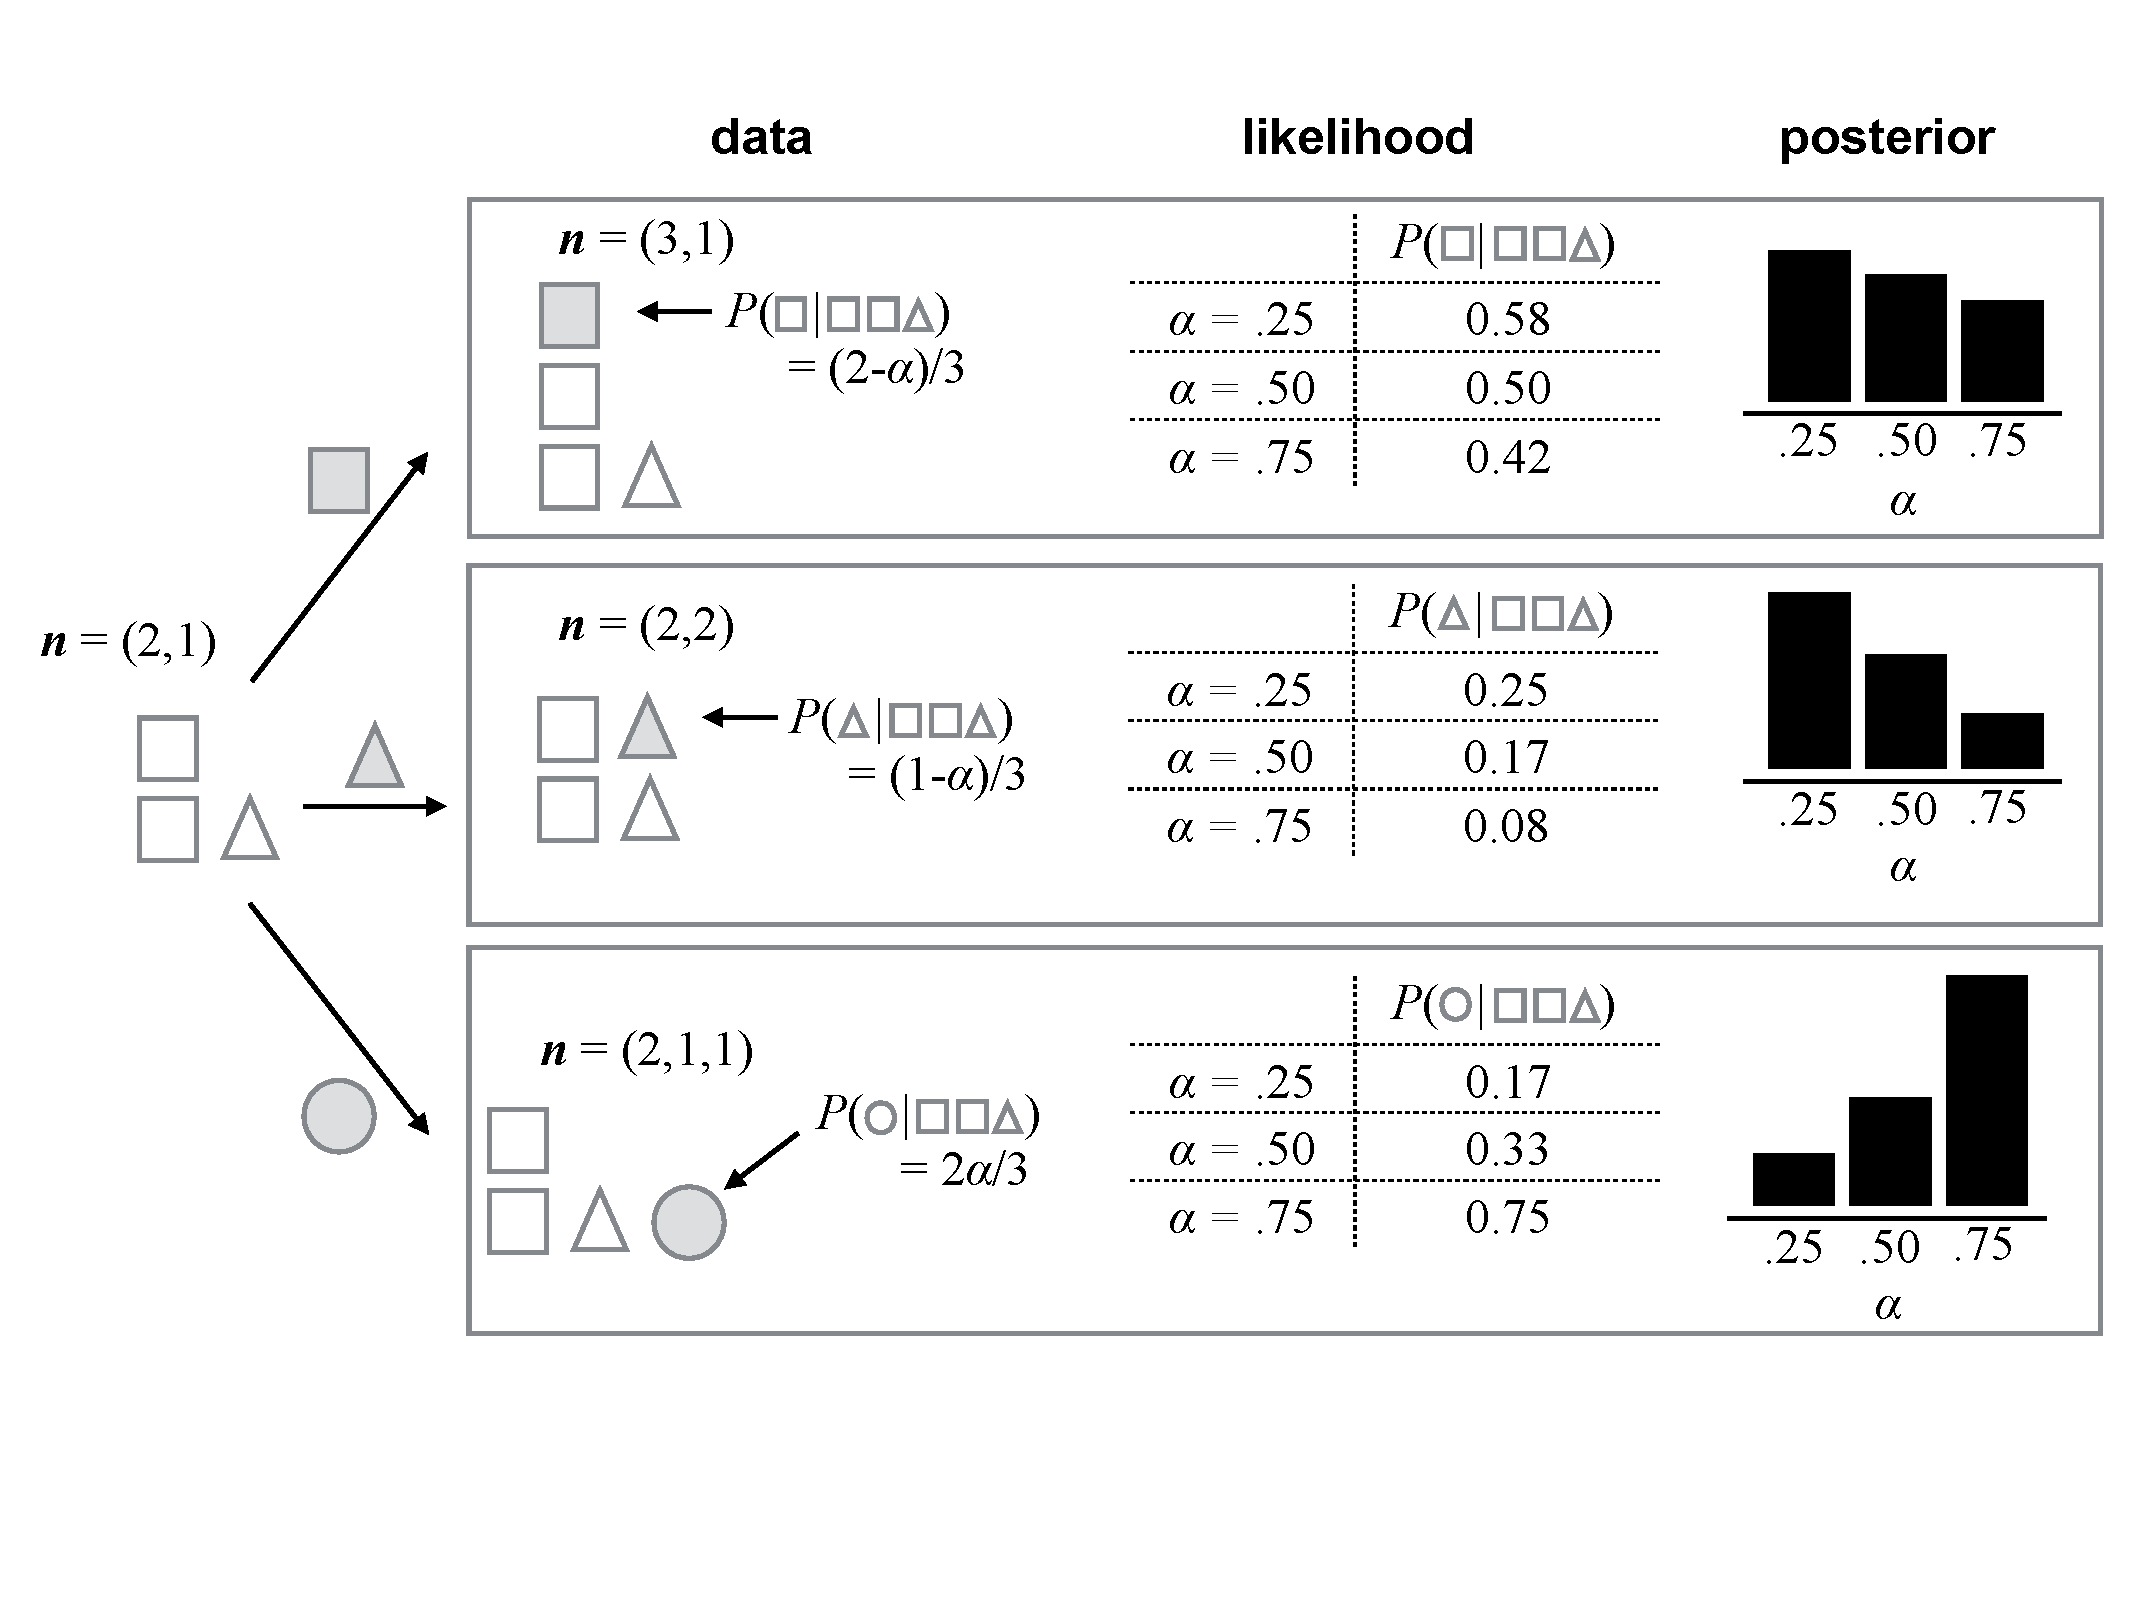
\includegraphics[scale=.4]{httr_inference.pdf}
\caption{An illustration of why the H-TTR model makes different inferences about $\alpha$ when presented with the frequency table \dist{31} than when it is given \dist{22}, even though both tables involve $N=4$ exemplars spread across $K=2$ categories. See main text for details. }
\label{fig:httr}
\end{center}
\end{figure}


\begin{figure}[p]
\begin{center}
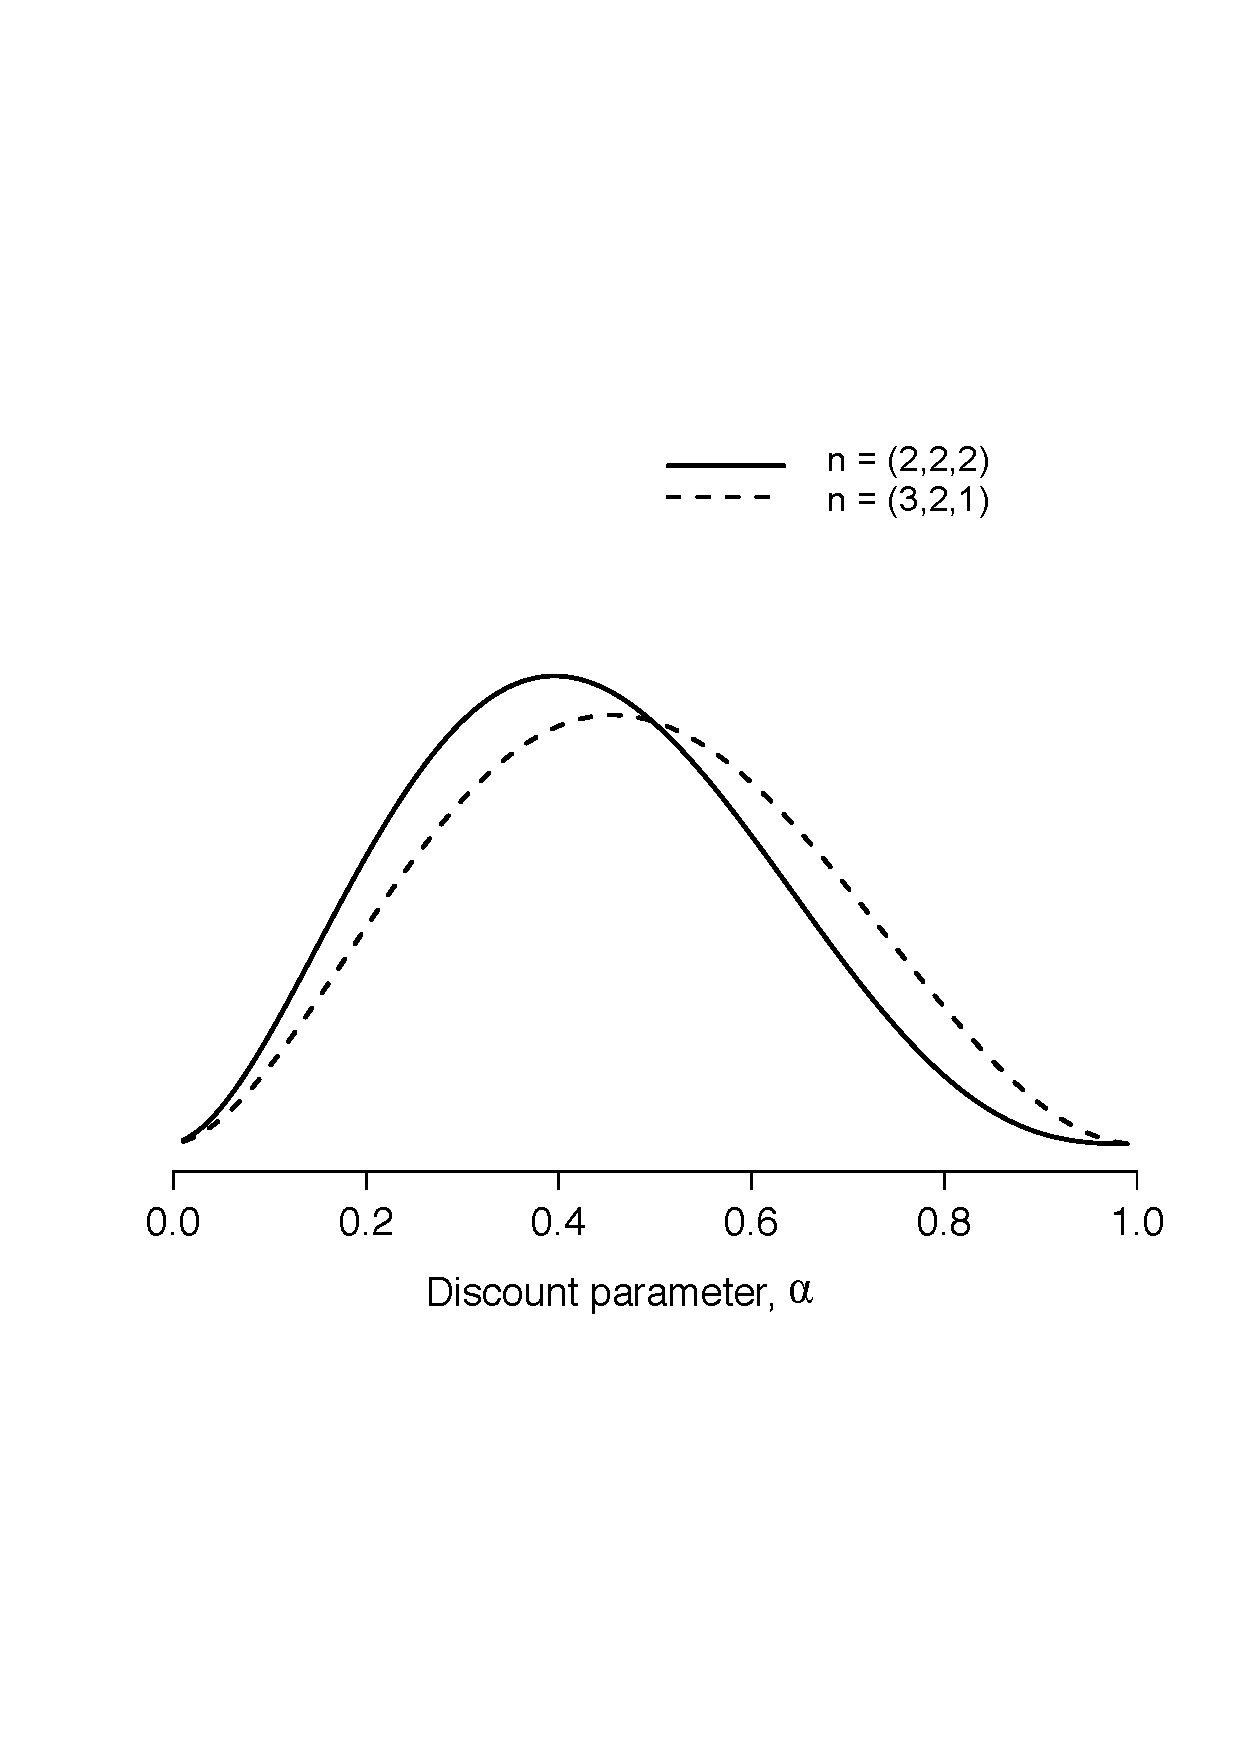
\includegraphics[scale=.35]{posteriorFig3a.pdf}
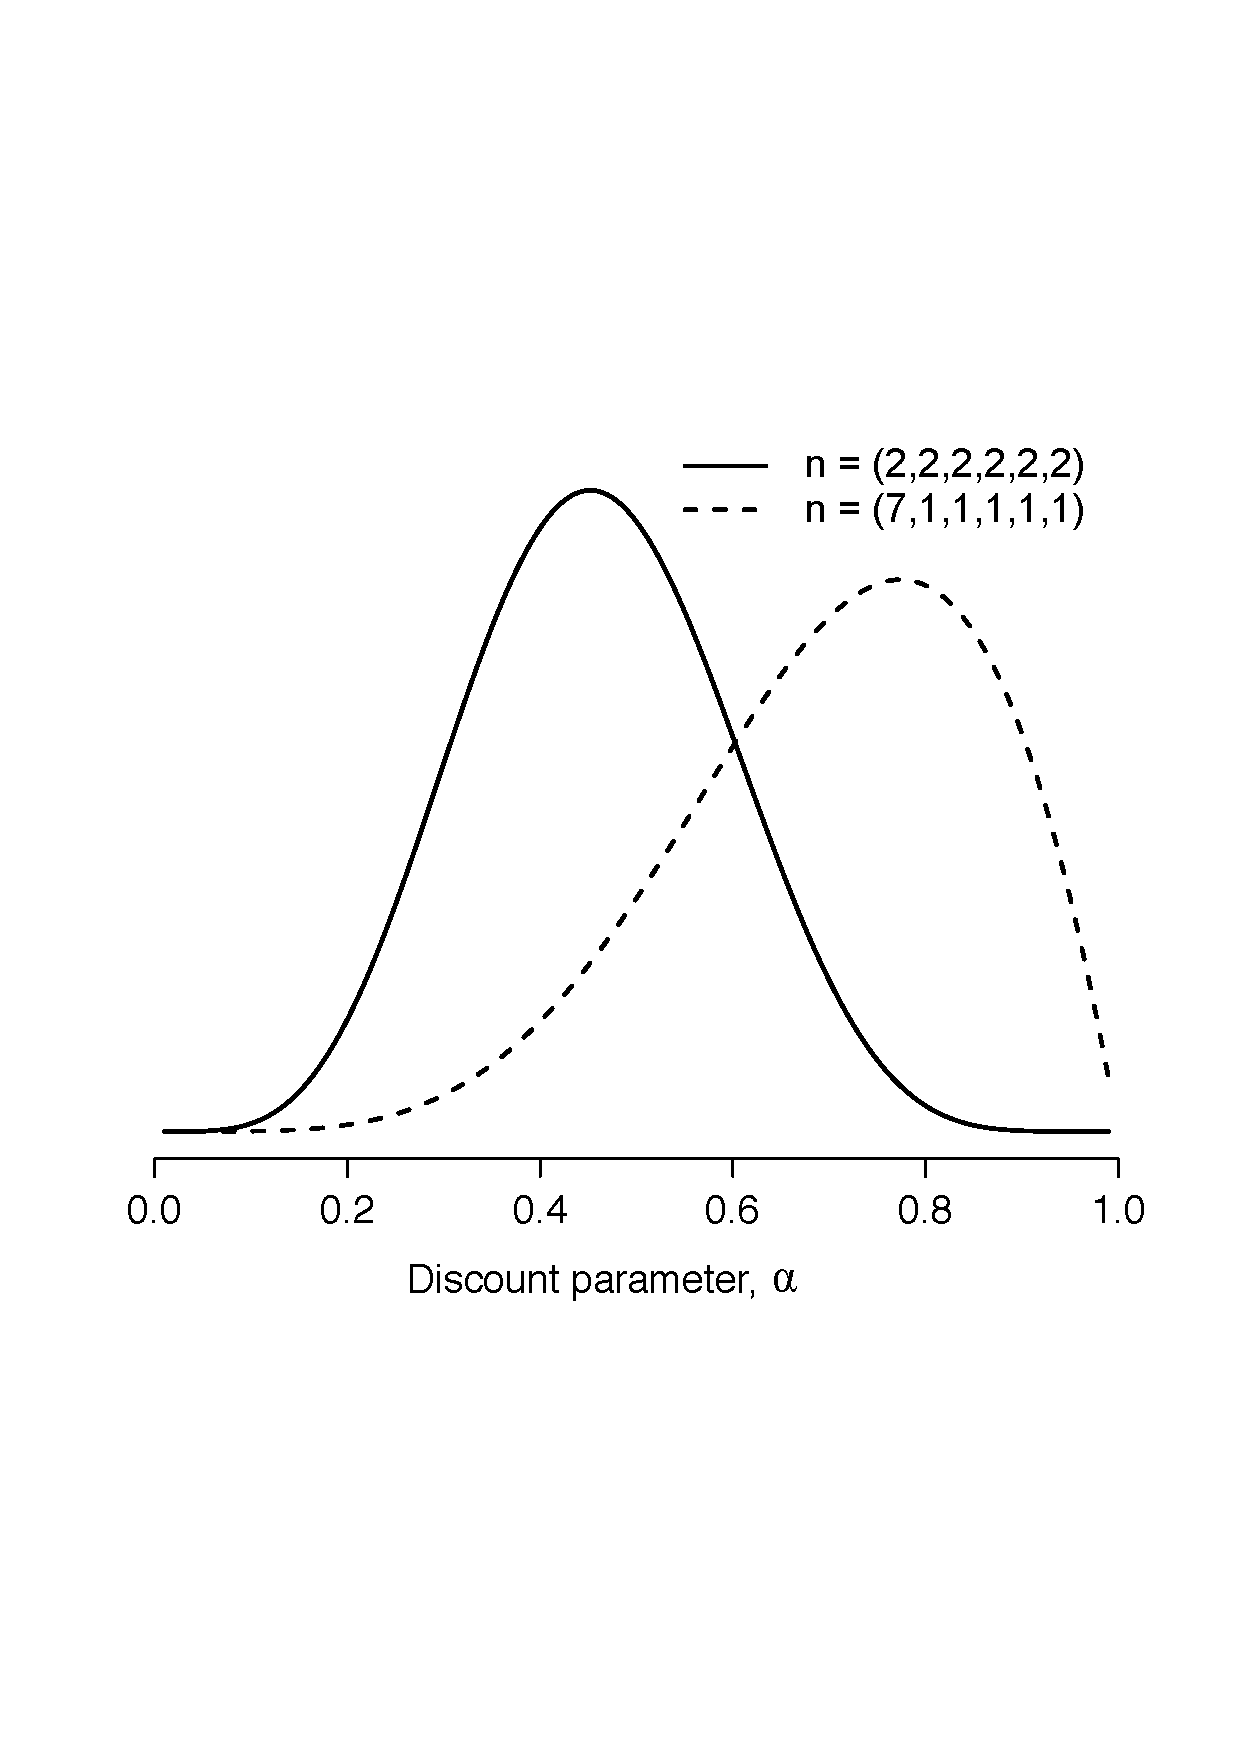
\includegraphics[scale=.35]{posteriorFig3b.pdf}
\caption{Posterior distribution over $\alpha$ in the H-TTR model for four different frequency tables. The prior in all four cases is a uniform distribution (i.e., $\beta_1 = \beta_2 = 1$).}
\label{fig:posteriors}
\end{center}
\end{figure}


Does this happen in practice? For the H-CRP model it is straightforward to prove that it does not (see Appendix). The posterior distribution $P(\theta |\bm{n})$ depends only on $N$ and $K$ and therefore the model cannot produce a transfer effect. For the other two models, both of which can learn the discount parameter $\alpha$, the situation is different. For the H-TTR model for instance, the posterior distribution $P(\alpha | \bm{n})$ depends on the entire frequency table, not merely the summary statistics $N$ and $K$. As a consequence the model can in some situations produce a transfer effect.

To understand why this happens, it is helpful to examine the mechanism by which the discount parameter $\alpha$ shapes the learner's belief updating within the G-CRP. When an observation appears from a novel category, the discount parameter describes how the ``strength'' associated with this observation is split between reinforcing the learner's beliefs that (a) this specific newly-discovered category will re-occur (b) yet another new category will appear. So far we have focused on (b), but (a) is equally important. In the simple CRP model a newly discovered category has strength 1 because it has been observed once. In the G-CRP model, however, the initial strength is only $1-\alpha$ because of the belief splitting mechanism described above. However, because all later exemplars of this category do not introduce a novel category, no such belief splitting occurs and so the difference in strength between the G-CRP model and the CRP attenuates. For example, the strength of a new category drops from 1 in the CRP to 0.2 in a G-CRP model with $\alpha = .8$, an 80\% reduction. Once 10 exemplars have been observed the difference is merely an 8\% reduction (from 10 to 9.2).

This simple mechanism has non-obvious implications, as spelled out in Figure~\ref{fig:httr}. The figure shows the entire inferential procedure for a variation of the H-TTR model in which the learner considers only three possible discount rates, corresponding to $\alpha$ values of 0.25, 0.50 and 0.75. For simplicity we imagine that this learner has observed two exemplars from category A and one from category B, yielding the \dist{21} frequency table shown on the left hand side of Figure~\ref{fig:httr}, and that the learner's current beliefs about $\alpha$ are uniformly divided between the three possible values. Using this simplified H-TTR model we consider what happens when the next observation arrives. There are only three possibilities: the next observation might belong to one of the two existing categories (A or B) or to a completely new one (C), so the frequency table will either become \dist{31}, \dist{22} or \dist{221}, as shown in the figure. The critical comparison is between the \dist{31} case and the \dist{22} case: if these differ in a systematic way, then the H-TTR model produces a transfer effect.

First consider the \dist{22} table. According to the TTR model, the probability that the next observation belongs to category B, thereby producing the \dist{22} table, is $(1-\alpha)/3$. The closer $\alpha$ is to 1, the closer this probability is to 0. So the likelihood function shown in the middle row of Figure~\ref{fig:httr} shows a strong bias: the observation is three times more probable when $\alpha = .25$ than when $\alpha = .75$. As a consequence, the learner's posterior over $\alpha$ shows a strong bias towards smaller values of $\alpha$. Now consider the \dist{31} table. The probability that the next observation belongs to category A -- thereby producing the frequency table 31 -- is $(2-\alpha)/3$. The likelihood that a new observation belongs to category A is far less sensitive to $\alpha$: when $\alpha = .75$ the observation is only 1.4 times as likely as it would be if $\alpha=.25$, so the evidence for small $\alpha$ is much weaker, and the corresponding posterior distribution is much flatter.

To summarize, uneven frequency tables are prima facie evidence for larger discount rates; and because larger values of $\alpha$ imply that more new categories are to be expected, any model that can {\it learn} the discount rate from data (i.e., H-TTR and HG-CRP) predicts that new categories are more likely when given an asymmetric table (e.g., \dist{31}) than when given a uniform table (e.g., \dist{22}) with the same number of exemplars and categories.


This raises a second question: if the H-TTR and HG-CRP models predict a transfer effect, why are they able to fit the data from Experiment 1 so effectively even though no such effect was observed empirically? It turns out that while these models do predict a transfer effect, the size of the predicted effect is very small for the frequency tables used in Experiment 1. This is illustrated for the H-TTR model in Figure~\ref{fig:posteriors}. The left panel depicts the posterior distribution $P(\alpha | \bm{n})$ for two different frequency tables used in Experiment 1, \dist{222} (solid lines) and \dist{321} (dashed line). Both of these frequency tables divide $N=6$ exemplars among $K=3$ categories, but the \dist{222} table divides the exemplars more evenly than the \dist{321} table. As the figure illustrates, a more uneven frequency distribution shifts the posterior distribution over $\alpha$ towards larger values as one would expect, but the effect size is very small. For a learner with a uniform prior over $\alpha$ (i.e., parameters $\beta_1 = \beta_2 = 1$), the predicted probability that the next observation represents a novel category is 22\% for the \dist{222} table, and 24\% for the \dist{321} table. Experiment 1 was not powered to detect an effect of that size. In contrast, the effect becomes much larger when more exemplars are shifted. The right panel of Figure~\ref{fig:posteriors} shows the comparison between the \dist{222222} table and the \dist{711111} table: transferring five exemplars in this fashion produces a much larger difference in what the learner infers about $\alpha$. In this instance, the H-TTR model predicts a 23\% chance of encountering a novel category when presented with the \dist{222222} table, and a 36\% chance when the table is \dist{711111}.


\section{Experiment 2}

The results of Experiment 1 provide strong evidence for the intuitively reasonable claim that familiar additions decrease the probability of a novel category, and novel additions increase that probability. This provides strong evidence that the CRP is inadequate as a model for human novelty detection, and modest evidence against the TTR and H-CRP models. However, as the previous discussion illustrates, Experiment 1 was not powered to detect a transfer effect. Given the theoretical relevance of such an effect, we designed a second experiment in which the transfer effect predicted by the H-TTR and HG-CRP models should be large enough to detect.

\subsection{Method}

\subsubsection{Participants} The study was completed by 200 workers on Amazon Mechanical Turk, who were paid US\$1.50 for their time (approximately 10 minutes). 196 participants were located in the United States, 3 in India and 1 in Venezuela. 98 self identified as male, 102 as female.

\subsubsection{Materials \& Procedure}

The frequency distributions used in Experiment 2 included all cases where the learner has seen exactly 12 exemplars divided among at least 2 and no more than 10 categories, subject to the restriction that there were at most  two distinct exemplar frequencies.\footnote{The reason for imposing this restriction was that there are 77 distinct frequency tables that can be produced by allocating 12 objects to categories. Our concern was that 77 conditions was too many to run, and we wanted a procedure for selecting a subset of these that would allow tests of the transfer effect without introducing a demand effect by calling attention to the hypothesis being tested.} This produces the 32 conditions listed in Table~\ref{tab:exp2}. The primary difference between conditions is the number of categories $K$ over which the 12 exemplars are distributed. However, for every value of $K$, the conditions can be (partially) ranked in terms relevant to the transfer effect in Figure~\ref{fig:intro}c. The \dist{9111} frequency table is deemed to be more unbalanced than the \dist{6222} table (and thus receives a higher rank) because we can produce the \dist{6222} condition by transferring exemplars ``down'' from high frequency categories to low frequency categories. Operationalized in this fashion, the \dist{6222} condition is neither above nor below the \dist{5511} condition because one exemplar must be transferred ``down'' and two exemplars transferred ``up'' to produce the \dist{5511} table from the \dist{6222} table. and accordingly they are assigned the same rank. We use this partial ranking over conditions to operationalize the transfer effect.


\begin{table}[t]
\caption{The 32 frequency distributions used in Experiment 2, listed as a function of the number of categories $K$. The vertical position of each object provides a partial ordering over frequency tables for each value of $K$. This ordering is derived by considering whether exemplars need to be transferred ``up'' or ``down'' in order to transform one table into another. Ties occur when exemplars need to be transferred in both directions. See main text for details.\vspace*{6pt}}
\label{tab:exp2}
\footnotesize
\begin{tabular}{c|rrrrrrrrr}
Rank &        $K=2$ &        $K=3$  &       $K=4$ &       $K=5$  &         $K=6$ &         $K=7$  &        $K=8$    &           $K=9$  &  $K=10$ \\ \hline
1&\dist{[11]1} & \dist{[10]11} & \dist{9111} & \dist{81111} & \dist{711111} & \dist{6111111} & \dist{51111111} & \dist{411111111} & \dist{3111111111} \\
2&\dist{[10]2} & \dist{822}    & \dist{5511} & \dist{42222} & \dist{441111} & \dist{2222211} & \dist{33111111} & \dist{222111111} & \dist{2211111111}  \\
 &             &               & \dist{6222} &              &               &                & \\
3&\dist{93}    & \dist{552}    & \dist{4422} & \dist{33222} &  \dist{333111}&                & \dist{22221111} \\
 &             & \dist{633}    &             &              &               \\
4&\dist{84}    & \dist{444}    & \dist{3333} &              & \dist{222222} \\
5&\dist{75}    &               &  \\
6&\dist{66} \\
\end{tabular}
\end{table}

\subsubsection{Exclusions} Clustering of individual subject responses produced the same qualitative pattern as in Experiment 1. The majority group consisted of 161 participants (80.5\%) whose responses all show strong positive correlations.In addition there were 20 participants (10\%) who appeared to reverse the response scale, and 19 participants (9.5\%) whose responses appear to be random. As before, we present data from the majority group, again noting that the averages taken across all participants are essentially identical to the majority.

\subsection{Results}

The empirical results and corresponding model fits are shown in Figure~\ref{fig:exp2}. Each panel plots the predictions of one model (grey bars) with the empirical data overlaid (black lines). Within each panel, the 32 frequency tables are divided up into groups consisting of all frequency tables that involve the same number of categories, and within each group the conditions are sorted by their rank as per Table~\ref{tab:exp2}.

Visual inspection of the plots reveals that the number of categories has a large effect, which is not surprising given the results of Experiment 1. As before, we tested effects using linear mixed models with the BayesFactor package in R, including fixed effects for the rank and the number of categories and a random effect of subject. Not surprisingly, we find an effect of the number of categories. Increasing the number of categories by one increased the  probability of a new category by 7.3\% on average, corresponding to a Bayes factor of approximately $10^{671}$ to 1 in favor of an effect. The CRP model again entirely fails to capture this qualitative effect, but all other models are able to capture it.

The theoretically interesting result is that Experiment 2 reveals a clear transfer effect. Within each group of conditions, responses decrease from left to right, consistent with the predictions of the H-TTR and HG-CRP models but not with the other four Bayesian accounts.\footnote{The slight within-block variation in the H-CRP model is caused by simulation error: were we able to compute the predictions of this model exactly these predictions would be flat. As noted earlier, the H-CRP model cannot produce any version of the transfer effect.} Again using linear mixed models to quantify the strength of evidence for this effect, we obtain overwhelmingly strong evidence (Bayes factor of approximately $10^9$) for a real transfer effect, but -- consistent with the models and with Experiment 1 -- the size of the effect is modest. The estimated effect of transferring a single exemplar from a high frequency category to a lower frequency one is to reduce the probability of new categories by 0.9\%, an effect size that would have been very difficult to detect in Experiment 1 given the smaller number of relevant comparisons and the drastically smaller differences that those comparisons entailed.



\begin{figure}[p]
\begin{center}
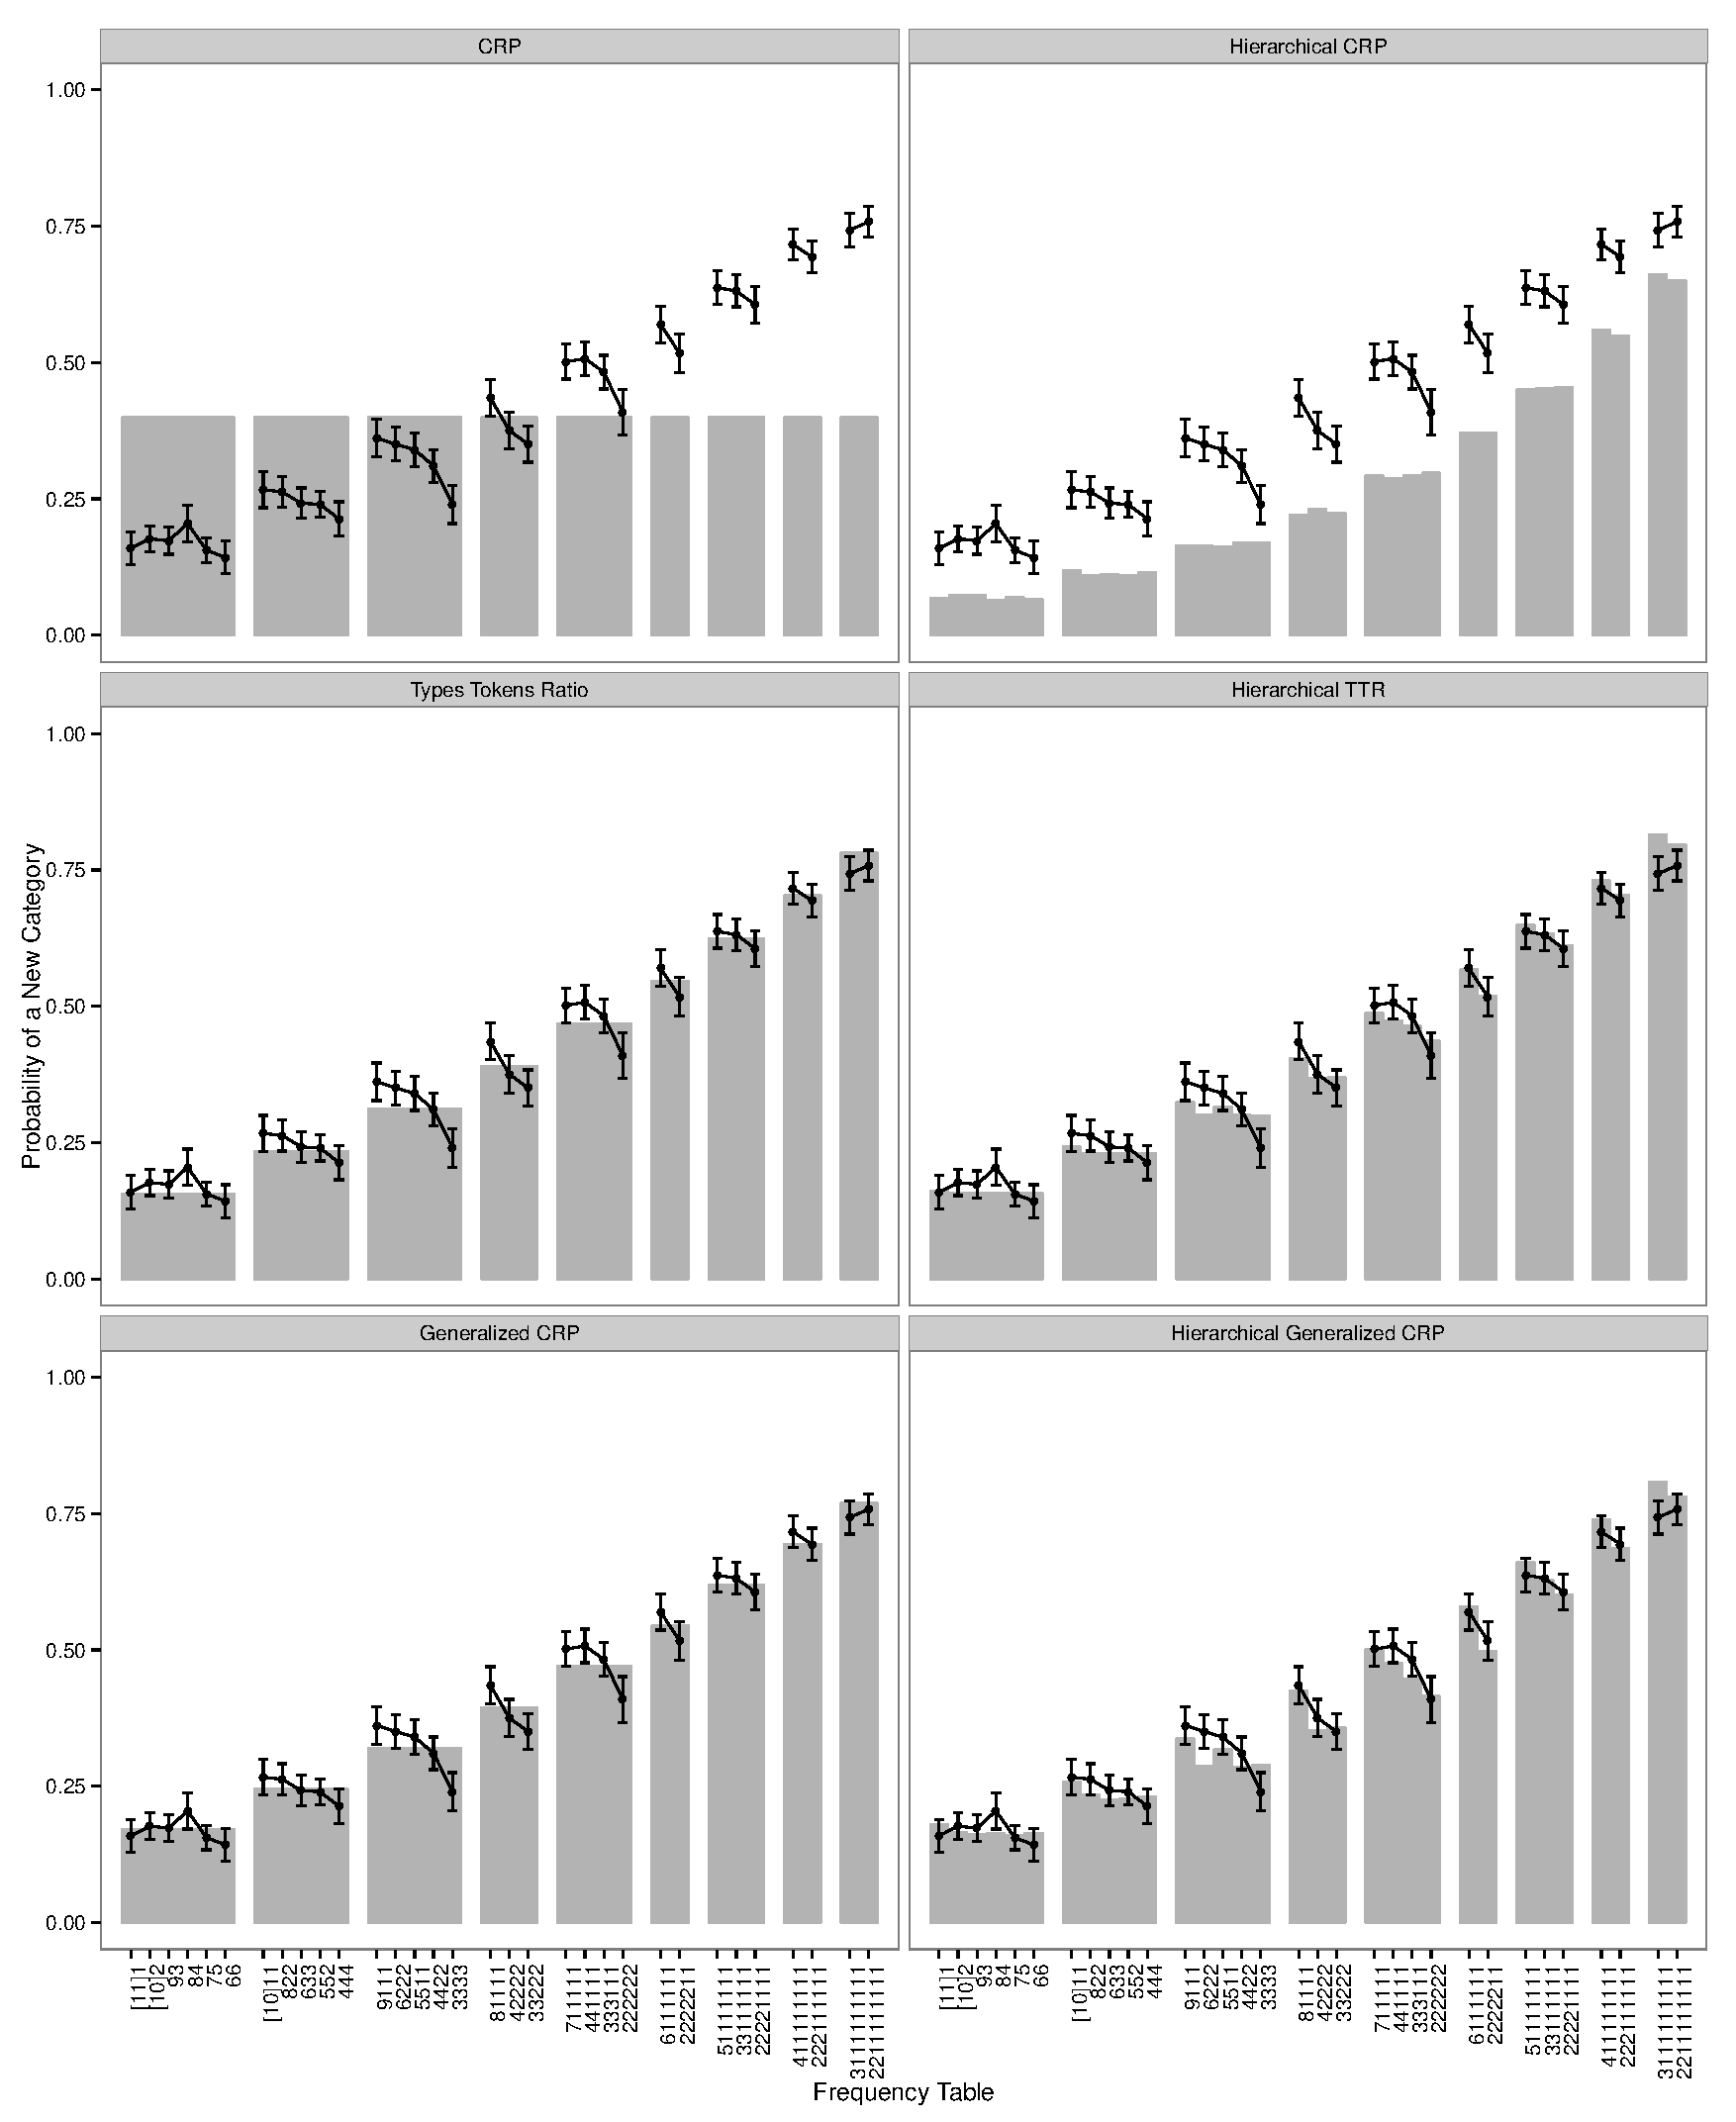
\includegraphics[scale=.55]{fit2.pdf}
\caption{Results from Experiment 2. The black lines plot mean responses for the human participants, with error bars corresponding to 95\% confidence intervals. The grey bars show the corresponding responses for all six Bayesian models at the best fitting parameter values.}
\label{fig:exp2}
\end{center}
\end{figure}


\begin{table}[t]
\caption{Parameter values for the three non-hierarchical Bayesian models (left) and three hierarchical Bayesian models (right) when fit to the data from Experiment 2.}
\label{exp2fits}
\vspace*{6pt}
\footnotesize
\begin{tabular}{cc}
\begin{tabular}{c|cc|c}
& \multicolumn{2}{c|}{Parameters} & \\
Model & Strength $\theta$ & Discount $\alpha$ & SSE \\ \hline
CRP & 7.97 &  & 1.147 \\
TTR &  & 0.94 & 0.030 \\
G-CRP & -0.25 & 0.92 & 0.027
\end{tabular}
&
\begin{tabular}{c|cc|cc|c}
& \multicolumn{2}{c|}{Prior over $\theta$} & \multicolumn{2}{c|}{Prior over $\alpha$}  \\
Model & Shape $\xi$ & Scale $\sigma$ & $\beta_1$ & $\beta_2$ & SSE \\ \hline
H-CRP & 1.54 & 9.83 & & & 0.643 \\
H-TTR & & & 36.72 & .154 & 0.021 \\
HG-CRP & 0.41 & 6.77 & 9.47 & 0.49 & 0.014
\end{tabular}
\end{tabular}
\end{table}

\subsection{Discussion}

The primary conclusion from Experiment 2 is that people's intuitions about the
probability of encountering a novel category are sensitive to more than the number of exemplars $N$ and the number of categories $K$: the {\it shape} of the frequency distribution matters also. Among the six Bayesian models that we proposed at the beginning of the paper, only two of them (H-TTR and HG-CRP) are capable of producing this effect. The CRP, TTR, G-CRP and H-CRP models all predict that inferences should depend solely on the total number of categories and the total number of exemplars, not on the manner in which exemplars are distributed across them.

One possible concern is that the hierarchical Bayesian approach is able to account for the data solely due to model flexibility. For example, in order to place priors over both $\theta$ and $\alpha$, the HG-CRP required us to specify four parameters ($\sigma$, $\xi$, $\beta_1$ and $\beta_2$). Given these four parameters, it is natural to wonder whether the HG-CRP model is flexible enough to capture any possible trend in the data. We addressed this concern by running a simulation study to check the robustness of the model predictions. Across the entire range of parameter values that we simulated (uniform distribution over [0,10] for all four parameters) the HG-CRP always predicts a negative effect of adding an exemplar to an category and a positive effect of adding an exemplar from a novel category. Similarly, it always predicts a transfer effect, but the effect is invariably much smaller than the other two effects, and at some parameter settings can be almost null. In short, despite having the most parameters of any model that we considered the HG-CRP model does not produce any qualitative pattern other than the one produced by human participants.




\section{Alternative models}

\begin{table}[p]
\caption{Eleven heuristics for the novelty detection problem. None of these models is capable of capturing all the qualitative trends in the data from Experiments 1 and 2.}
\label{heuristicsfail}
\small
\begin{itemize}
\item {\it Smallest frequency}. The learner's response is proportional to the frequency of the lowest frequency category. This model fails because it cannot account for systematic effects among conditions with the same minimum frequency (e.g., \dist{11}$<$\dist{111}$<\ldots<$\dist{111111}). See panel (a) of Figure~\protect\ref{heuristicpics}.
\item {\it Largest frequency}. As above, but the response is based on the modal category. This model does not account for systematic effects among conditions with the same maximum frequency (e.g., \dist{11}$<$\dist{111}$<\ldots<$\dist{111111}). Plotted in panel (b) of Figure~\protect\ref{heuristicpics}.
\item {\it Largest versus smallest}. The response is based on the difference (or ratio) between the most frequent and least frequent category. It cannot produce systematic effects among conditions when the maximum and minimum are identical (e.g., \dist{11}$<$\dist{111}$<\ldots<$\dist{111111}, \dist{21}$<$\dist{211}$<\ldots<$\dist{21111}). The difference model is shown in panel (c) and the ratio model in panel (d).
\item {\it Tokens minus types}. A variation of the TTR model in which the response is based on the difference between the number of exemplars and the number of categories rather than the ratio. It cannot predict any version of the transfer effect in Experiment 2. Shown in panel (e).
\item {\it Singleton count/proportion}. The response is based on the number (or proportion) of categories that have frequency 1. This model does not account for systematic effects when exemplars are added to the modal category (e.g., \dist{21}$>$\dist{31}$>$\dist{41}$>$\dist{51}). The number version is plotted in panel (f) and the proportion version in panel (g).
\item {\it Small category count}. The response is in proportion to the number (or proportion) of categories with frequency $k$ or less, where $k$ is a free parameter. This model cannot produce a smooth trend when exemplars are added to the modal category  as in \dist{11}$>$\dist{21}$>\ldots>$\dist{51}. It (incorrectly) produces a discontinuity at the value of $k$. For example, at $k=3$ it predicts \dist{11}$=$\dist{21}$=$\dist{31}$<$\dist{41}$=$\dist{51}. Best fitting model predictions are shown in panels (h) and (i).
\item {\it Number of exemplars in small categories}. The response is proportional to the number of exemplars belonging to small categories, where small is defined via a threshold frequency $k$. Many observed effects require different values of $k$. For instance, capturing \dist{311}$>$\dist{32} requires $k=1$ whereas capturing \dist{311}$>$\dist{411} requires $k=3$. The model cannot capture these effects simultaneously. Shown in panel (j).
\item {\it Proportion of exemplars in small categories}. As above, but defined in terms of the proportion of exemplars in categories with frequency $k$ or below, rather than the absolute number. This model cannot predict systematic effects when all categories have the same frequency (e.g., \dist{1}$<$\dist{11}$<\ldots<$\dist{111111}, \dist{2}$<$\dist{22}$<$\dist{222}). Shown in panel (k).
\end{itemize}
\end{table}


\begin{figure}[p]
\footnotesize
\begin{tabular}{|cc|cc|}
\hline
\multicolumn{2}{|l|}{(a) Smallest frequency} & \multicolumn{2}{l|}{(b) Largest frequency} \\
\raisebox{-2cm}{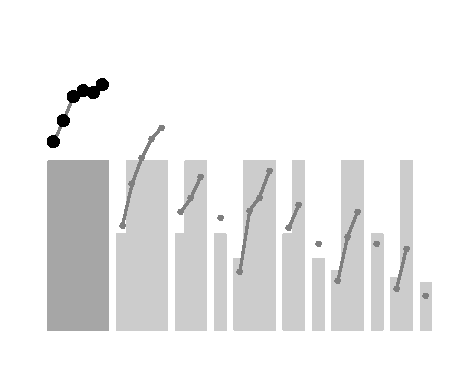
\includegraphics[width=\miniplotsize]{./mod1exp1.pdf}} &
\raisebox{-2cm}{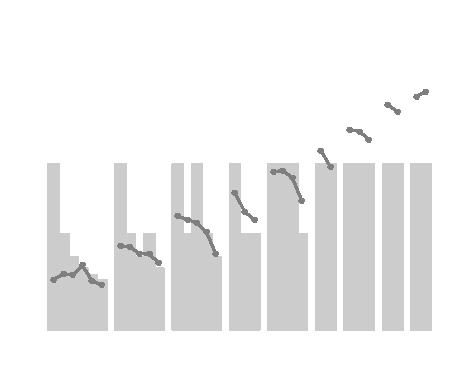
\includegraphics[width=\miniplotsize]{./mod1exp2.pdf}} &
\raisebox{-2cm}{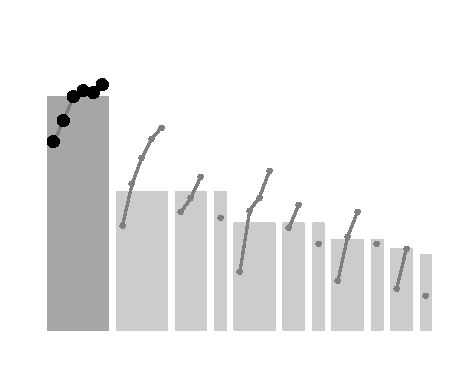
\includegraphics[width=\miniplotsize]{./mod2exp1.pdf}} &
\raisebox{-2cm}{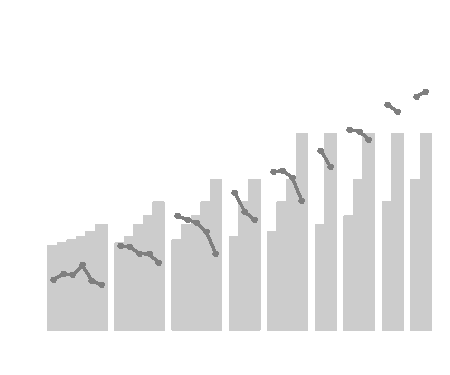
\includegraphics[width=\miniplotsize]{./mod2exp2.pdf}} \\ \hline
\multicolumn{2}{|l|}{(c) Largest minus smallest} & \multicolumn{2}{l|}{(d) Largest to smallest ratio} \\
\raisebox{-2cm}{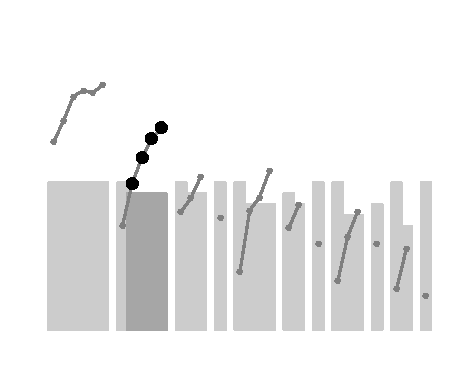
\includegraphics[width=\miniplotsize]{./mod3exp1.pdf}} &
\raisebox{-2cm}{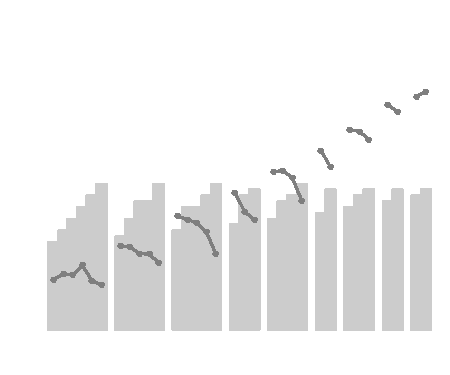
\includegraphics[width=\miniplotsize]{./mod3exp2.pdf}} &
\raisebox{-2cm}{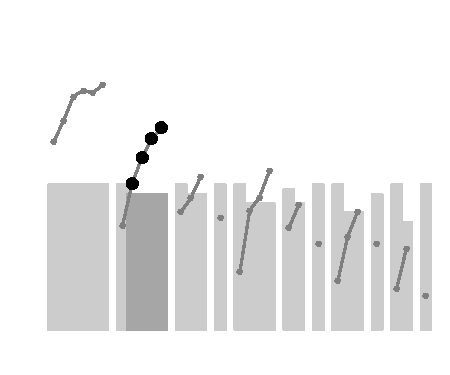
\includegraphics[width=\miniplotsize]{./mod4exp1.pdf}} &
\raisebox{-2cm}{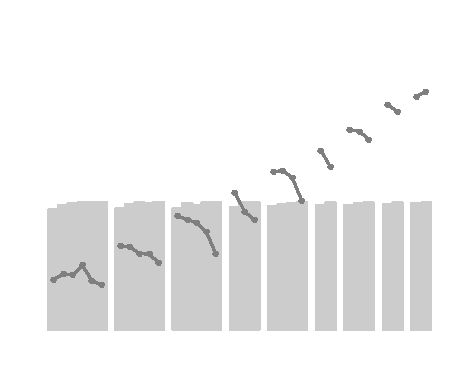
\includegraphics[width=\miniplotsize]{./mod4exp2.pdf}} \\ \hline
\multicolumn{2}{|l|}{(e) Tokens minus types} & \multicolumn{2}{l|}{(f) Singleton count} \\
\raisebox{-2cm}{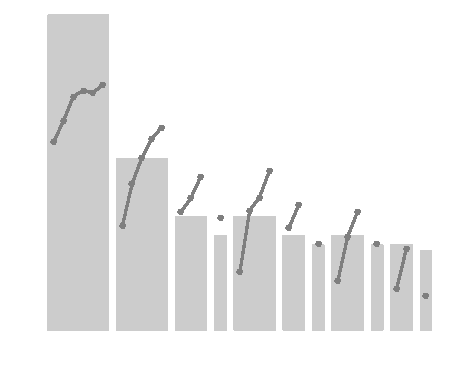
\includegraphics[width=\miniplotsize]{./mod5exp1.pdf}} &
\raisebox{-2cm}{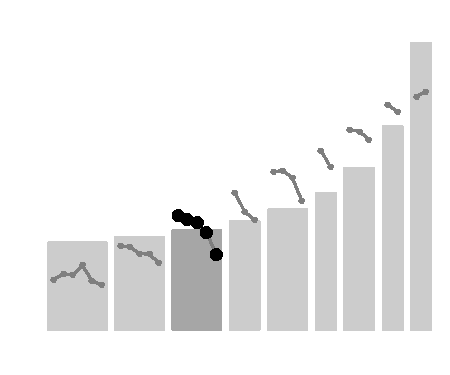
\includegraphics[width=\miniplotsize]{./mod5exp2.pdf}} &
\raisebox{-2cm}{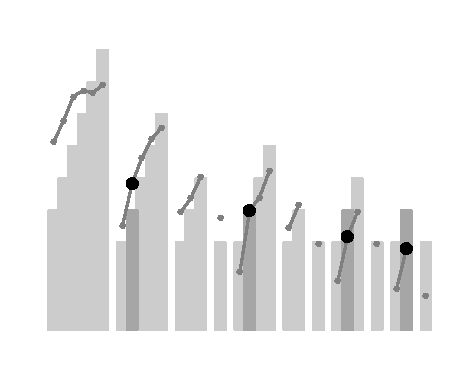
\includegraphics[width=\miniplotsize]{./mod7exp1.pdf}} &
\raisebox{-2cm}{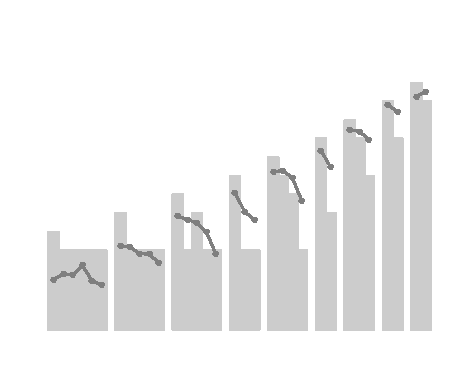
\includegraphics[width=\miniplotsize]{./mod7exp2.pdf}} \\ \hline
\multicolumn{2}{|l|}{(g) Singleton proportion} & \multicolumn{2}{l|}{(h) Small category count} \\
\raisebox{-2cm}{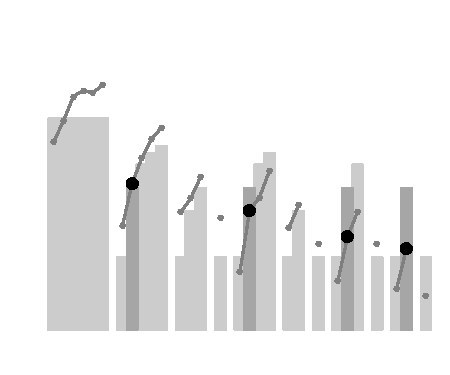
\includegraphics[width=\miniplotsize]{./mod8exp1.pdf}} &
\raisebox{-2cm}{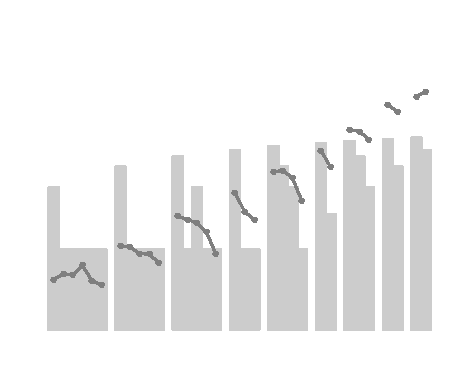
\includegraphics[width=\miniplotsize]{./mod8exp2.pdf}} &
\raisebox{-2cm}{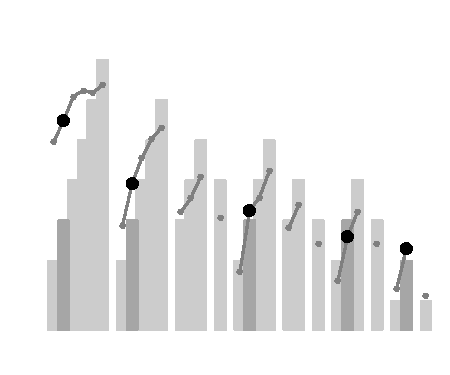
\includegraphics[width=\miniplotsize]{./mod9exp1.pdf}} &
\raisebox{-2cm}{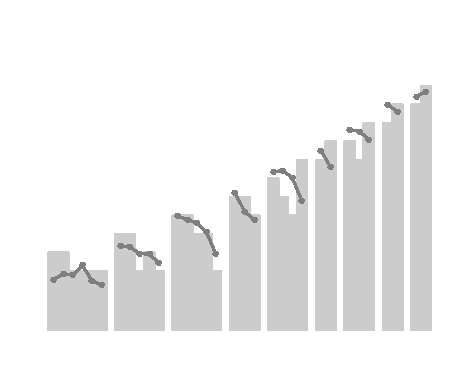
\includegraphics[width=\miniplotsize]{./mod9exp2.pdf}} \\ \hline
\multicolumn{2}{|l|}{(i) Small category proportion} & \multicolumn{2}{l|}{(j) Number of exemplars in small categories} \\
\raisebox{-2cm}{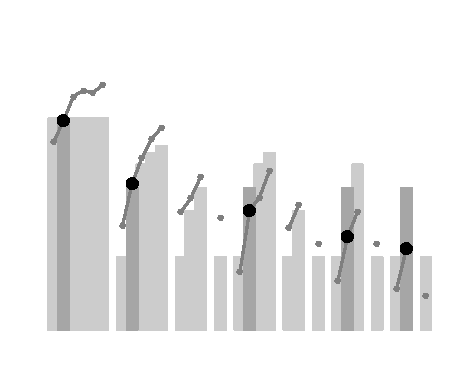
\includegraphics[width=\miniplotsize]{./mod10exp1.pdf}} &
\raisebox{-2cm}{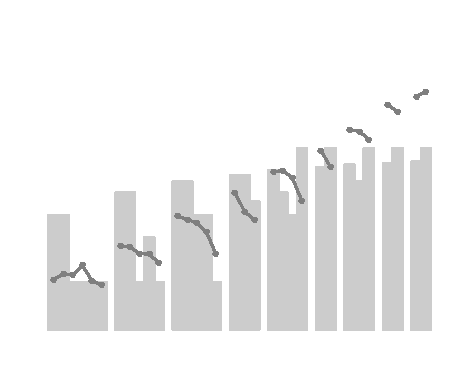
\includegraphics[width=\miniplotsize]{./mod10exp2.pdf}} &
\raisebox{-2cm}{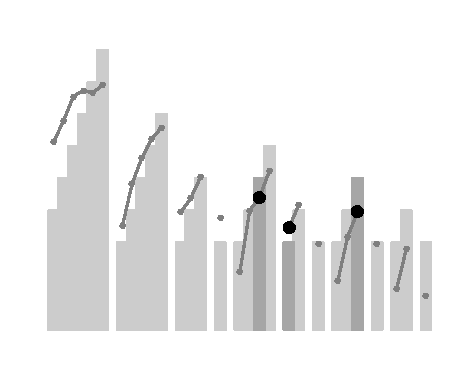
\includegraphics[width=\miniplotsize]{./mod11exp1.pdf}} &
\raisebox{-2cm}{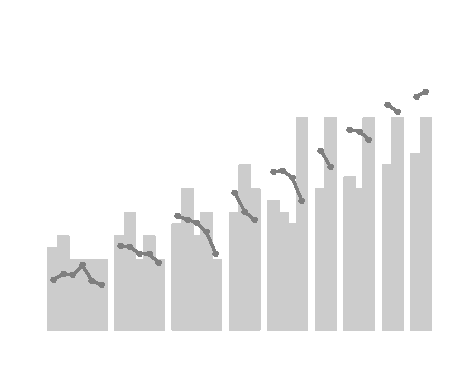
\includegraphics[width=\miniplotsize]{./mod11exp2.pdf}} \\ \hline
\multicolumn{2}{|l|}{(k) Proportion of exemplars in small categories} & \multicolumn{2}{l|}{(l) Simplicity model} \\
\raisebox{-2cm}{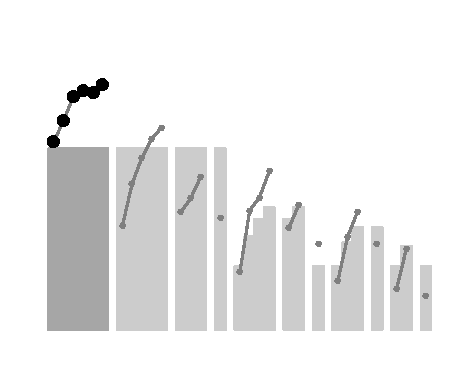
\includegraphics[width=\miniplotsize]{./mod12exp1.pdf}} &
\raisebox{-2cm}{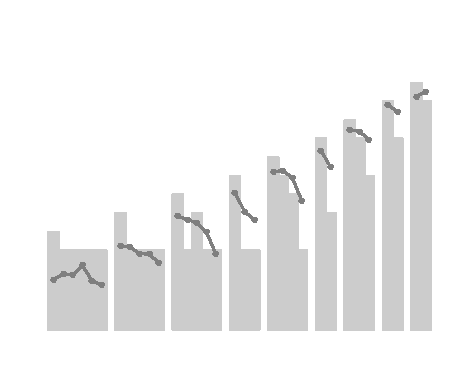
\includegraphics[width=\miniplotsize]{./mod12exp2.pdf}} &
\raisebox{-2cm}{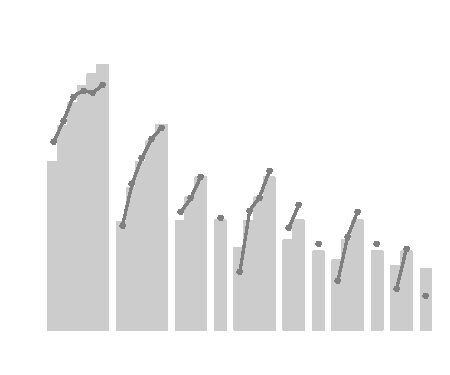
\includegraphics[width=\miniplotsize]{./mod15exp1.pdf}} &
\raisebox{-2cm}{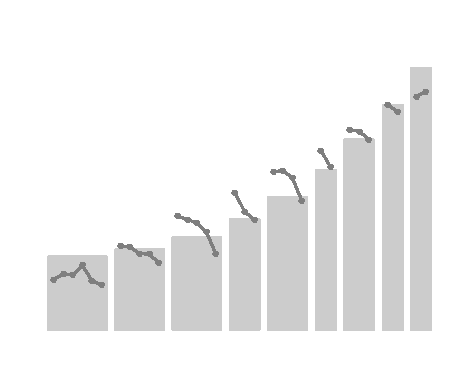
\includegraphics[width=\miniplotsize]{./mod15exp2.pdf}} \\  \hline
\multicolumn{4}{c}{}
\end{tabular}
\caption{Predictions of all eleven heuristics listed in Table~\protect\ref{heuristicsfail} and the simplicity model for Experiments 1 (left) and 2 (right).
In each case, the highlighted conditions illustrate the particular qualitative failure of the heuristic described in the corresponding entry in Table~\protect\ref{heuristicsfail}.
To put the model predictions on the same scale as the human data, each set of predictions was passed through a linear regression function with a slope parameter and an intercept parameter. In addition to these two parameters, some of the heuristics have an extra free parameter as described in Table~\protect\ref{heuristicsfail}. All free parameters were set by minimizing sum squared error.}
\label{heuristicpics}
\end{figure}

So far we have considered six Bayesian models that are all related to Anderson's rational model (1991). Our results suggest that capturing the three key effects (familiar addition, novel addition, transfer) is not simple: of the six models we considered, only two can do so. We now consider the extent to which several non-Bayesian approaches can account for our data.

\subsection{Heuristic models}

Table~\ref{heuristicsfail} lists 11 possible heuristics that can be applied to Experiments 1 and 2. In each case the heuristic is fairly intuitive, but nevertheless fails to capture at least one theoretically important qualitative trend in the data, as the table illustrates. In addition, Figure~\ref{heuristicpics} shows that each heuristic fails to produce a good quantitative fit to the data.
It is of course impossible to rule out every possible heuristic, and better fits might be possible if multiple heuristics are combined, but the results challenge the idea that there is a single, simple heuristic that will account for our data. Human intuitions about the novelty detection problem seem to be a good deal more sophisticated than simple heuristic models would imply.

\subsection{Exemplar models}

If simple heuristics cannot mimic human performance on these problems, how do existing categorization models fare? One very successful family of categorization models assumes that the learner stores all previously observed exemplars in memory, and categorizes new objects by assessing the similarity between old objects and new ones. The generalized context model \cite<GCM;>{nosofsky_attention_1986} is the best known of these exemplar models. According to the GCM, the probability that a new object belongs to the $k$-th old category is proportional to the sum of its similarities to the other objects known to belong to that category:
\begin{equation}
P(l_{N+1} = k) \propto \sum_{j|l_{j} = k} \mbox{sim}(x_{N+1},x_j)
\label{eq:gcm}
\end{equation}
where $\mbox{sim}(\cdot,\cdot)$ is a function that measures the similarity between two objects, and the normalizing term is found by summing across all old categories. For Experiments 1 and 2 we did not show people any object features, merely the labels. Without any observable stimulus features other than the label, the similarity function $\mbox{sim}(\cdot,\cdot)$ is difficult to specify, but it seems reasonable to assume that the similarities are constant for any pair of objects. If so, then the response strength for any given category is proportional to the number of exemplars:
\begin{equation}
P(l_{N+1} = k) \propto n_k
\label{eq:gcm2}
\end{equation}
The fundamental difficulty in applying the GCM is that Equation~\ref{eq:gcm2} does not provide a mechanism by which a response strength can be assigned to a novel category. If there are no stored exemplars, the response strength according to the GCM is zero. A natural way to adapt the GCM is suggested by \citeA{nosofsky_tests_1991} who applied a variation of the model to recognition memory experiments: an object is labelled as ``new'' if the summed similarity to all exemplars is below some criterion level of familiarity. On that basis one might argue that this criterion level can also serve as a response strength for a novel category. However, this approach produces a model in which the response strength is proportional to sample size for all old categories, and described by a fixed response strength for novel categories: in other words, the CRP.

The fact that an extended GCM ends up equivalent to Anderson's rational model (and fails for the same reasons) is perhaps unsurprising, given that the connection between the GCM and the rational model has been discussed elsewhere in the literature \cite<e.g.,>{nosofsky_relation_1991,nosofsky1998optimal}. However the connection we have drawn here is somewhat different and slightly more general, in a fashion that is closely connected to the novelty detection problem itself. The derivation presented by \citeA{nosofsky_relation_1991} shows that the original GCM is equivalent to Anderson's model only when the coupling parameter $c$ is set to 0  (i.e., $\theta \rightarrow \infty$) during the training phase of an experiment and then shifts to $c=1$  (i.e., $\theta = 0$). In many situations this inconsistency does not matter, but for novelty detection it is critical: the strength parameter $\theta$ provides the mechanism by which the RMC is able to detect novel categories, and it is exactly with respect to this parameter that the correspondence between exemplar models and Anderson's model breaks down. Our suggestion, in contrast, is that the GCM can be extended by connecting the novelty detection problem to recognition memory, but that even this extended GCM fails in the same fashion as Anderson's original formulation of the RMC.

Finally, it is worth noting that the shortfalls of this version of the GCM are not necessarily fatal to exemplar models generally. For example, \citeA{stanton_category_2013} describe an exemplar model in which the ``background noise'' parameter scales with the number of categories $K$, and \citeA{nosofsky_short-term_2011} describe one in which it scales with the number of exemplars $N$. Plausibly, these mechanisms could be adapted to produce a version of the GCM that behaves similarly to the G-CRP model, and additional theoretical development could potentially yield a model that produces human-like transfer effects as the H-CRP and HG-CRP models do.


\subsection{Connectionist models}

An alternative approach to categorization relies on connectionist networks. For example, the ALCOVE model \cite{kruschke_alcove:_1992} is a connectionist network that extends the GCM, and fails to address the novelty detection problem because -- like the GCM -- it relies on the summed similarity rule in Equation~\ref{eq:gcm} to form response strengths and does not have a mechanism for assigning strength to a never-before-seen category. Other connectionist models, however, do not share this reliance on the summed similarity rule. SUSTAIN~\cite{love_sustain:_2004}, for example, is a connectionist model that represents categories in terms of a set of clusters. It begins with a single cluster that includes a single object, and can introduce new categories as subsequent objects are encountered. During supervised classification tasks SUSTAIN does not have a mechanism for recruiting new clusters until after feedback is provided, and in that sense it cannot solve the novelty detection problem in the sense we have described it (i.e., rejecting all previous labels and deciding that a new category is needed).

However, SUSTAIN does provide a mechanism for cluster recruitment in an unsupervised learning context that is somewhat more relevant to the problem. Specifically, a new category is introduced if the similarity between the current object and the closest existing category lies below a threshold, denoted $\tau$. Unfortunately this solution does not accommodate our results. Again working from the assumption that that the similarity is roughly constant (because participants were only shown arbitrary labels) the fact that $\tau$ is constant across learning is problematic: it implies that SUSTAIN would make identical predictions about every condition in our Experiments 1 and 2. Alternatively, just as we considered a hierarchical version of the CRP that can learn the strength parameter, it should be possible to develop a hierarchical version of SUSTAIN that can learn the $\tau$ parameter in the same way that it learns other unknown quantities (i.e., gradient descent on error). Extending SUSTAIN in this way may allow it to account for our results, but it is not obvious (to us at least) what specific assumptions would be required to make this work. For the present purposes, it suffices to note that the standard version of the model does not capture the qualitative effects in our data.


\subsection{Connecting novelty detection to unsupervised categorization}

Of the categorization models discussed so far, SUSTAIN and Anderson's model are the only two that offer solutions to the novelty detection problem without requiring extensive modification. They are also the only two models that can perform unsupervised categorization as well as supervised categorization. This is not coincidental, because there is a formal connection between unsupervised learning and novelty detection, which we now outline.

Unsupervised categorization is the problem of
organizing a set of objects into a system of categories $S$, and formal
approaches to this problem can typically be understood in terms of a
function that measures the goodness of a category system $g(S)$.
The novelty detection problem can be connected to unsupervised learning
as follows. Suppose that the learner has encountered a set of $N$
objects known to be categorized into a system $S_N$ that contains $K$
categories. When the next observation arrives the learner can assign
it to one of the $K$ existing categories or to a new category $K+1$.
Deciding whether a new object belongs to a novel category is a
matter of comparing the goodness of the system that assigns the object to
a new category to the goodness of systems that assign the object to an
existing category. Formally, if $S_N^k$ denotes the category system that
would result if the new object were assigned to the $k$-th category,
the probability of the learner doing so can be calculated using the
Luce choice rule,
\begin{equation}
P(l_{N+1} = k) = \frac{g(S_N^k)}{\sum\limits_{i=1}^{K+1} g(S_N^i)}
\label{lucegoodness}
\end{equation}
where $g(\cdot)$ is the goodness function. As long as the goodness function
is well-defined for every category system $S$, the corresponding unsupervised
learning model can be converted into a model of novelty detection using
Equation~\ref{lucegoodness}.

\subsection{Unsupervised GCM and the simplicity model}

Besides SUSTAIN and Anderson's model, there are at least two other unsupervised categorization models that we might consider adapting via Equation~\ref{lucegoodness}, namely the simplicity model~\cite{pothos_simplicity_2002} and the unsupervised GCM~\cite{pothos_predicting_2009}. The unsupervised GCM (uGCM) turns out to be inapplicable to our data, because it does not define a goodness function $g(\cdot)$ that is well-defined for the category systems of interest. To see why, note that the uGCM measures the goodness of a category system by taking each object out of the system and using the regular GCM to predict how it should be categorized. A system is considered good to the extent that the GCM predicts the correct label of each held-out object with high confidence. However, because the original GCM does not have a mechanism for introducing novel categories, the uGCM does not have a mechanism for scoring the goodness of any system in which some categories contain a single object only. Despite being an unsupervised learning model the uGCM is not applicable to the novelty detection problem for exactly the same reason that the GCM is inapplicable: it relies on similarity to stored exemplars.

The final model that we consider is the simplicity model \cite{pothos_simplicity_2002}, which develops a goodness function based on information theoretic considerations. The simplicity model proposes that good category systems have simple descriptions, where ``simple'' in this instance means ``short''. The descriptions considered are two-part codes: the first part specifies a grouping of objects into categories, and the second part specifies similarities among objects given this grouping into categories. The overall goodness of a system is defined as the sum of the lengths of these codes. We combined this goodness function with Equation~\ref{lucegoodness} to generate the model predictions shown in Figure~\ref{heuristicpics}l (additional details can be found in the Appendix). The simplicity model performs relatively well, and achieves an overall sum-squared error that is lower than the errors achieved by the best heuristic model. The model, however, is unable to capture the transfer effect in Experiment 2.  The model predicts that the probability of encountering a new category depends only on the number of objects and the number of categories encountered thus far, and therefore makes identical predictions about each group of conditions in the right plot of Figure~\ref{heuristicpics}l.


\subsection{Summary}

The alternative models considered here do not exhaust the set of possible novelty detection models. Our discussion of these alternatives, however, illustrates that it is surprisingly difficult to capture the qualitative trends and quantitative results from Experiments 1 and 2. To the best of our knowledge, there is no existing psychological model that can match the performance of the H-TTR and the HG-CRP models, nor is there an obvious alternative to them at this stage.


\section{Experiment 3}

The Bayesian approach to categorization outlined in Equation~\ref{basicbayes} relies on the prior $P(l_{N+1} | \bm{l}_{1:N})$ to form expectations about the rates with which different categories will appear, and because this prior is shaped by the frequency table $\bm{n}$ our experimental work has focused on the way in which different frequency tables influence people's prior expectations. In order to isolate the effect of frequency information from the effect of similarity, Experiments 1 and 2 presented people only with a set of arbitrary labels. However, most category learning experiments do provide people with information about stimulus similarity, as do most everyday categorization problems. The Bayesian framework is well suited to capture similarity effects through the likelihood  $P(x_{N+1} | \bm{x}_{1:N}, \bm{l}_{1:N})$, as discussed by Anderson (1991), and in light of the importance of similarity to categorization it is important to investigate how similarity influences the novelty detection problem.

Previous work has suggested that object frequency and stimulus similarity have independent effects on categorization \cite{nosofsky_similarity_1988}, and so one might expect that models that performed well in Experiments 1 and 2 should continue to do so when similarity is introduced as a factor. However, given that previous work did not consider the novelty detection problem (i.e., object frequency effects were considered only with respect to exemplars of old categories), it is important to consider how similarity and frequency distribution interact in this situation. Experiment 3 used a standard supervised categorization design to explore how frequency information affects novelty detection when similarity information is also present.

\subsection{Method}

\subsubsection{Participants} The study was completed by 400 workers on Amazon Mechanical Turk, who were paid US\$0.75 for their time (approximately 7 minutes). Data were not received for 1 participant. Among the remaining 399 participants, 368 participants were located in the United States, 24 in India and 7 elsewhere. 214 self identified as male, 184 as female and 1 did not answer.

\subsubsection{Materials \& Procedure} There were 12 sets of stimuli that varied along a single stimulus dimension, one per condition. The stimulus sets are depicted in Figure~\ref{fig:stim3}. An initial calibration study was used to keep the discriminability of the different stimulus sets fairly similar, but given variations in individual thresholds and in the testing conditions across workers using different machines, the more important control was that the assignment of stimulus sets to logical conditions was randomized across subjects.


\begin{figure}[p]
\begin{center}
\footnotesize
\begin{tabular}{c|cccccccc}
Value & Set 1 & Set 2 & Set 3 & Set 4 & Set 5 & Set 6 \\ \hline
 \\
 \raisebox{.75cm}{55} &

\includegraphics[scale=\stimulusscale]{./set1stim55.png} &
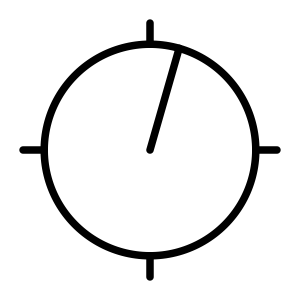
\includegraphics[scale=\stimulusscale]{./set2stim55.png} &
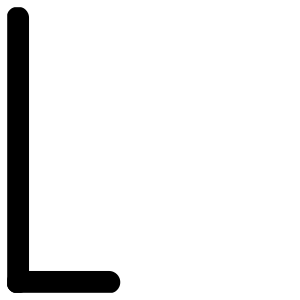
\includegraphics[scale=\stimulusscale]{./set3stim55.png} &

\includegraphics[scale=\stimulusscale]{./set4stim55.png} &
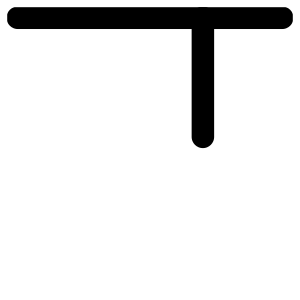
\includegraphics[scale=\stimulusscale]{./set5stim55.png} &
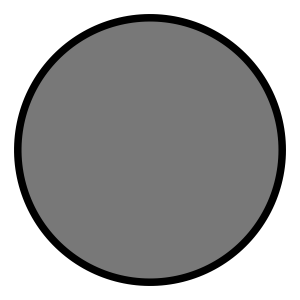
\includegraphics[scale=\stimulusscale]{./set6stim55.png} \\[6pt]
 \raisebox{.75cm}{75}  &

\includegraphics[scale=\stimulusscale]{./set1stim75.png} &
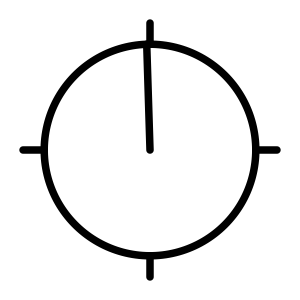
\includegraphics[scale=\stimulusscale]{./set2stim75.png} &
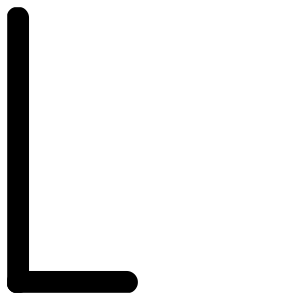
\includegraphics[scale=\stimulusscale]{./set3stim75.png} &

\includegraphics[scale=\stimulusscale]{./set4stim75.png} &
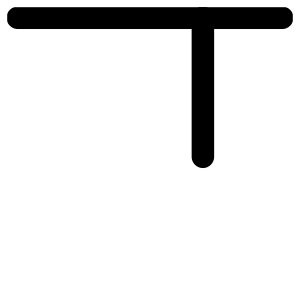
\includegraphics[scale=\stimulusscale]{./set5stim75.png} &
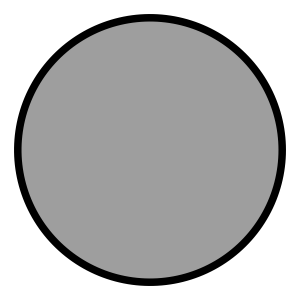
\includegraphics[scale=\stimulusscale]{./set6stim75.png} \\
\multicolumn{1}{c}{}\\
\multicolumn{1}{c}{}\\
Value & Set 7 & Set 8 & Set 9 & Set 10 & Set 11 & Set 12 \\[6pt] \hline
\\
 \raisebox{.75cm}{55}  &

\includegraphics[scale=\stimulusscale]{./set7stim55.png} &

\includegraphics[scale=\stimulusscale]{./set8stim55.png} &

\includegraphics[scale=\stimulusscale]{./set9stim55.png} &

\includegraphics[scale=\stimulusscale]{./set10stim55.png} &

\includegraphics[scale=\stimulusscale]{./set11stim55.png} &

\includegraphics[scale=\stimulusscale]{./set12stim55.png}\\[6pt]
 \raisebox{.75cm}{75}  &

\includegraphics[scale=\stimulusscale]{./set7stim75.png} &
\includegraphics[scale=\stimulusscale]{./set8stim75.png} &
\includegraphics[scale=\stimulusscale]{./set9stim75.png} &
\includegraphics[scale=\stimulusscale]{./set10stim75.png} &
\includegraphics[scale=\stimulusscale]{./set11stim75.png} &
\includegraphics[scale=\stimulusscale]{./set12stim75.png} \\
\end{tabular}
\caption{The stimuli used in Experiment 3 consisted of 12 different sets of objects that varied along one dimension. Examples of each stimulus set are depicted above, showing the stimuli with values of 55 and 75 on the scale depicted in Figure~\protect\ref{fig:design3}. }
\label{fig:stim3}
\end{center}
\end{figure}

\begin{figure}[p]
\begin{center}
\includegraphics[scale=.55]{design3.pdf}
\caption{The design of Experiment 3 involved 6 different category structures, each corresponding to a different frequency table. For each category structure there were two test locations, one near to the training items and one more distant, yielding a total of 12 distinct conditions. See main text for details.}
\label{fig:design3}
\end{center}
\end{figure}

The logical design of the experiment is shown in Figure~\ref{fig:design3}. There were 6 distinct exemplar frequency distributions, corresponding to the \dist{11}, \dist{111}, \dist{1111}, \dist{21}, \dist{31} and \dist{211} conditions from Experiment 1. As Figure~\ref{fig:design3} illustrates, there is always a critical category (category A) that consists of a single exemplar located at stimulus value 75 (see Figure~\ref{fig:stim3}). All other training exemplars, regardless of which category they belonged to (categories B, C and D) were located at value 60 or below, and their locations were chosen in order to convey the sense that categories were relatively homogeneous. There were two critical test items, one located at stimulus value 85 (the near object) and the other at 95 (the far object). The 6 frequency distributions and 2 similarity levels produced 12 within-subject conditions, completed by participants in a random order.\footnote{There were minor failures of randomization in this experiment caused by a coding error. These issues were rectified for the replication in Experiment 4, and the close agreement between the two experiments suggests any distortions caused by randomization issues were modest.}

The cover story introduced the categorization task by explaining to participants that their goal was to learn about an alien language. As before, the instruction set explained the interface and the procedure, and participants had to correctly answer three instruction check questions before being allowed to proceed with the task. In each condition participants were shown the training stimuli in a random order followed by one test item. Each condition consisted of several trials, in which participants were required to predict the label of the most recently presented item and were provided with feedback at the end of every trial, except for the test trial.

Within each condition, the trials proceeded as follows. At the start of each condition the first stimulus was displayed with the category label printed underneath. Labels were three letter nonsense words (e.g, ``dax'') that were never repeated across conditions and randomized across participants. The second object was then displayed next to the first, with no label shown (question marks were shown instead). Participants were given the option of indicating that the second object belonged to the same category as the first one, by pressing a button displaying the relevant category name, or guessing that it belonged to a new category by pressing a button that read ``new''. After making their choice, the correct label  -- sometimes one of the previously encountered labels and sometimes a new one -- was revealed underneath the object, replacing the question marks.\footnote{Note that the instruction set explicitly discussed the ``new'' button, and explained that ``new'' was in fact the correct answer whenever the true label turned out to be different from any previously observed one.} After a 1 second delay, the next object was presented adjacent to the previous ones with question marks underneath and the response options updated if a new category label had just been introduced. A screenshot showing the experiment in progress (on the second trial of one condition) is shown in Figure~\ref{fig:display3}.

Within each condition, all objects remained on screen for the entire task, ensuring that when the test item was shown on the final trial, all training items and their labels were available. The test item was not announced, ensuring that the participants had no reason to think that this trial would be any different to the preceding ones. No feedback was given on the test item. Indeed, the reason for having one test item per condition rather than two was to ensure that people did not learn anything from the test items, nor recognize that there were any special test items at the end.


\subsubsection{Exclusions} As in Experiments 1 and 2 we used correlations among participant responses to determine if we could detect qualitative patterns of individual difference, taken only across the 12 test judgments: order effects in presentation mean that these are the only responses that are comparable across individuals.  No patterns of individual differences were found which is perhaps not surprising. The simplicity of the task ensured that people could not ``reverse'' the response scale as sometimes happened in Experiments 1 and 2, and the fact that each participant provided only 12 judgments limits the ability to detect people responding randomly. We therefore include data from all 399 participants in the analysis.


\begin{figure}[p]
\begin{center}
\includegraphics[scale=.25]{display3.png}
\caption{A screenshot showing Experiment 3 in progress. The task on this trial is to classify the object on the right. The response buttons allow the participant to assign the object to one of the existing categories (i.e., ``pas'' or ``foo'') or to guess that it represents a ``new'' category whose label is not yet known.}
\label{fig:display3}
\end{center}
\end{figure}

\begin{figure}[p]
\begin{center}
\includegraphics[scale=.5]{data3.pdf}
\caption{Data from Experiment 3, showing the proportion of participants assigning the test item to a novel category (left column), to the nearest old category (middle column), or to one of the other categories (right column). The top row shows the classification probabilities for the near test items, and the bottom row shows the corresponding probabilities for the far test items. Within each panel, responses are plotted separately for each of the six category structures.}
\label{fig:exp3data}
\end{center}
\end{figure}


\subsection{Results}

The data of interest are people's responses on the test items, plotted in Figure~\ref{fig:exp3data} for all 12 conditions. Almost invariably, participants assigned the test item either to a new category (61\% of responses) or to the nearest old category (category A was chosen on 34\% of occasions). The more distant categories (B, C and D) were chosen only on 5\% of trials. While unsurprising, the fact that people treated the test trial as a comparison between category A and ``new'' places constraints on  possible models.

It is clear that similarity information plays an important role in deciding whether to assign the test item to a novel category. As one might expect, a novel object that is very dissimilar to all old objects is more likely to be assigned to a novel category than a new object that closely resembles a familiar one. That is, when deciding whether to assign a test item to category A or a new category, people were more likely to select ``new'' for the far test item (71\%) than for the near one (47\%). Using a Bayesian linear mixed effects model, the Bayes factor indicates that the evidence for the effect is approximately $10^{101}$ to 1.

Moreover, similarity does override frequency in some instances. Increasing the number of exemplars in the most distant category has very little influence on people's willingness to assign the novel object to that category: for instance, in the \dist{31} condition category B has three exemplars whereas in the \dist{11} condition it has only one. The fact that all exemplars of category B are very dissimilar to the test items (near or far) ensures that increasing the frequency of category B has a very limited effect on people's willingness to select it.

Frequency, however, does play a very strong role in people's willingness to endorse a novel category, and in a quite sophisticated way. The left hand side of Figure~\ref{fig:exp3data} shows that increasing the frequency of category B {\it does} have a large effect, although this effect has nothing to do with the endorsement of category B. Rather, the effect is to change the relative willingness to choose category A instead of  a novel category. This is a somewhat curious variation of the familiar addition effect: consistent with Experiments 1 and 2, the probability of a new category decreases across the sequence of conditions \dist{11}\goesto\dist{21}\goesto\dist{31} and \dist{111}\goesto\dist{211} relative to the probability of choosing category A, even though category A consists of a single exemplar in every case. The Bayes factor for this effect is $10^{141}$ to 1.

Changes to the frequency table that affect the number of categories are a little more complicated in this design. The sequences \dist{31}\goesto\dist{211}\goesto\dist{1111} and \dist{21}\goesto\dist{111} are constructed by taking exemplars from (relatively nearby) category B and creating the somewhat more distant categories C and D. Doing so has the effect of increasing people's willingness to assign test items to a novel category (Bayes factor: $10^{44}$ to 1). This effect is not surprising, because the frequency distribution and similarity information are in agreement. Moving exemplars in this fashion increases the number of categories (a distributional effect) but also makes the training exemplars more distinct from the test item (a similarity effect).

A different test can be constructed by examining the sequences \dist{11}\goesto\dist{111}\goesto\dist{1111} and \dist{21}\goesto\dist{211} in which  the number of exemplars and the number of categories increase. This is broadly analogous to the novel addition effect discussed in connection with Experiments 1 and 2, though the analogy is closer for the \dist{11}\goesto\dist{111}\goesto\dist{1111} sequence in which the locations and category memberships of old objects do not change when the new object is added. Curiously, although several models predict that the willingness to endorse a novel category should increase across these sequences (discussed later) and this effect was observed in previous experiments, it is attenuated to the point of absence in Experiment 3 with no systematic effect being observable. Close inspection of Figure~\ref{fig:exp3data} suggests that the 11-near condition is somewhat anomalous (Bayes factor of 25:1 favoring a model that includes a specific term for the ``11-near'' condition) with people generalizing more readily in that condition than would be expected on the basis of all the other results, but even if that condition is excluded the evidence weakly favors a null effect (Bayes factor: 8:1) across these sequences.

\subsection{Novelty detection models that integrate similarity and frequency}

\begin{figure}[t]
\begin{center}
\includegraphics[scale=.5]{similarities.pdf}
\caption{Likelihood functions for all three categories in the \dist{211} condition in Experiment 3. These likelihoods describe the learner's beliefs about which stimulus features are most likely to be generated when objects are sampled from each category, and depend on both the training exemplars (shown at the bottom of the figure) and the learner's priors about category features. The parameters used to generate these plots are the same ones used to fit the HG-CRP model (see Table~\protect\ref{exp3fits}). The probability distribution associated with the novel category is denoted ``new'', and is roughly uniform across the admissible range of stimulus values (see main text).}
\label{fig:exp3likelihood}
\end{center}
\end{figure}

The empirical results suggest that people integrate similarity information (based on observable features) and distributional information (carried by the frequency table), and do not rely solely on one or the other. Even a cursory inspection of Figure~\ref{fig:exp3data} reveals that models that rely solely on the similarity between the nearest category and the test item (e.g., SUSTAIN) will be unable to accommodate the empirical results because such models should predict that all six frequency distributions produce the same results. Moreover, because the nearest category always has the same frequency (i.e. $n=1$), any successful model must use the frequency information in a way that is more sophisticated than simply weighting each old category by its observed frequency.

Each of the six Bayesian models described earlier can be applied to
supervised classification tasks in which the stimulus features are observable. To do so we need a likelihood function that describes the probability that a stimulus would be observed with feature values $x_{N+1}$ given that it comes from category $k$. For continuous valued features, we follow Anderson \citeyear{anderson_adaptive_1991} and assume that each category produces a normal distribution.\footnote{The model used here is not identical to Anderson's model. Anderson (1991) draws a distinction between categories (or clusters), which define a joint probability distribution over stimulus features, and category labels, which are assumed merely to be an additional feature. Because of this distinction, it is possible under some parameterizations for a single category label to map onto multiple categories, or in other instances for a single category to be associated with multiple labels. However, as Anderson (1991) noted, many simple experimental designs -- such as those depicted in Figure~\protect\ref{fig:design3} -- tend to produce a one-to-one mapping between labels and categories across a wide range of parameter values (see \citeNP{griffiths_unifying_2007}). This does create some ambiguity insofar as it is not always clear whether people are inferring novel categories or novel labels, but it should be noted that Bayesian analyses that pertain to labels specifically (e.g., \citeNP{VongPerforsNavarro2016}) have also tended to use the CRP prior for the label prediction problem.} In this approach each category is described in terms of the mean $\mu$ and variance $\sigma^2$, though it will be convenient to parameterize the variability of the category in terms of the precision $\tau = 1/\sigma^2$. Given this specification, the learner places priors $P(\mu,\tau)$ over the mean and precision, and for each category infers the posterior distribution
\begin{equation}
P(\mu_k,\tau_k \given \bm{x}_k) \propto P(\bm{x}_k \given \mu_k, \tau_k) P(\mu_k, \tau_k)
\end{equation}
where we use the notation $\bm{x}_k$ to refer to the features of only those exemplars that belong to category $k$.\footnote{A more precise way to denote this would be $\bm{x}_{i|l_i=k}$, in order to be consistent with the previous notation $\bm{x}_{1:N}$ in which the subscript picks out the indices of the relevant exemplars. We hope that our intended meaning will be clear from context.} As discussed in the Appendix, we use standard normal-gamma priors over the category distribution parameters. That is, the learner assumes that the precision $\tau$ is drawn from a gamma distribution, and the mean $\mu$ is drawn from a normal distribution. One nice property of this prior is that the learner's beliefs can be characterized in terms of four interpretable parameters:
\begin{itemize}\setlength{\parskip}{0pt}
\item $\mu_0$ is the learner's best {\it a priori} guess for the category mean $\mu$
\item $\tau_0$ is the learner's best {\it a priori} guess for the category precision $\tau$
\item $n_\mu$ is a pseudo-count indicating how much weight to place on $\mu_0$
\item $n_\tau$ is a pseudo-count indicating how much weight to place on $\tau_0$
\end{itemize}
In our applications we fixed $\mu_0=60$ to be the mean of the empirical observations and $n_\mu=.001$. However, because the parameters $\tau_0$ and $n_\tau$ have an important role to play in specifying how widely the learner generalizes from a small sample, we treat these as free parameters to be estimated.

Because the learner does not know the true parameters associated with the category, the likelihood function for the featural information is given by the marginal probability,
\begin{equation}
P(x_{N+1} \given l_{N+1} =k,\bm{x}_{1:N}, \bm{l}_{1:N}) = \int P(x_{N+1} \given \mu_k, \tau_k ) P( \mu_k, \tau_k \given \bm{x}_{k} ) \ d(\mu_k, \tau_k)
\end{equation}
which in this instance corresponds to a $t$ distribution and can be calculated analytically (see Appendix). Our model adapts this integral by truncating the range of $x_{N+1}$, ensuring that the likelihood function only assigns positive probability to feature values within a range that would fit on the screen. For objects assigned to a ``new'' category, the marginal probability is calculated by integrating over the prior $P(\mu,\tau)$ rather than a posterior $P(\mu,\tau | \bm{x})$. To give a sense of how this model behaves, Figure~\ref{fig:exp3likelihood} plots the likelihood function $P(x_{N+1} \given l_{N+1} =k,\bm{x}_{1:N}, \bm{l}_{1:N}) $ for all three old categories in the \dist{211} condition, as well as the likelihood function associated with a novel category.

As with previous experiments, we estimated model parameters using a simulated annealing procedure to minimize sum squared errors between the model response probabilities and the empirical ones. Data fitting was done at the level of specific responses (i.e., A, B, C, D or ``new'') and the best fitting parameter values and corresponding SSE values are shown in Table~\ref{exp3fits}. However, since the most interesting empirical results all pertain to the probability of classifying the stimulus as ``new'', Figure~\ref{fig:exp3} plots the model predictions only for those cases.


\begin{table}[t]
\caption{Parameter values for the three non-hierarchical Bayesian models (top) and three hierarchical Bayesian models (bottom) when fit to the data from Experiment 3. For the similarity component, the prior mean was fixed as $\mu_0 = 60$ and the weight attached to this mean was fixed to be equivalent to $n_\mu =.001$ observations, reflecting a strong {\it a priori} assumption that the locations of categories are unknown. The priors associated with the precision were treated as free parameters, because these influence the width of generalization gradients in each category.}
\label{exp3fits}
\vspace*{6pt}
\footnotesize
\begin{tabular}{c}
\begin{tabular}{c|cc|cc|c}
& \multicolumn{2}{c|}{Prior parameters} &   \multicolumn{2}{c|}{Likelihood parameters} &\\
Model & Strength $\theta$ & Discount $\alpha$ & Precision $\tau_0$ & Weight $n_\tau$ & SSE \\ \hline
Uniform & & & .95 & .00 & .29 \\
CRP & .21 &  & .68 & .52 & .27 \\
TTR &  & .12 & .36 & .39 & .23 \\
G-CRP & .058 & .089 & .32 & .41 & .22
\end{tabular}
\\ \\
\begin{tabular}{c|cc|cc|cc|c}
& \multicolumn{2}{c|}{Prior over $\theta$} & \multicolumn{2}{c|}{Prior over $\alpha$}  &   \multicolumn{2}{c|}{Likelihood} &\\
Model & Shape $\xi$ & Scale $\sigma$ & $\beta_1$ & $\beta_2$ & Precision $\tau_0$  & Weight $n_\tau$  & SSE \\ \hline
H-CRP & .28 & 2.02 & & & .015 & 4.47 & .12 \\
H-TTR & & & 5.69 & 7.60 & .02 & 5.60 & .19 \\
HG-CRP & .73 & 1.61 & .12 & 4.09 & .016 & 6.27 & .06
\end{tabular}
\end{tabular}
\end{table}

\begin{figure}[t]
\begin{center}
\begin{tabular}{cc}
\includegraphics[scale=.5]{fit3_flat.pdf} &
\includegraphics[scale=.5]{fit3_hierarchical.pdf}
\end{tabular}
\caption{Performance of the six Bayesian models when fit to the data from Experiment 3. All three non-hierarchical models fail to produce the same qualitative trends as human participants. All three hierarchical models produce the correct qualitative trend, with HG-CRP producing the best quantitative fit.}
\label{fig:exp3}
\end{center}
\end{figure}



\subsection{The importance of hierarchical priors}

Figure~\ref{fig:exp3} and Table~\ref{exp3fits} reveal that although none of the Bayesian models provides a perfect account of the data, some perform worse than others. In particular, the three models that rely on a non-hierarchical prior (CRP, TTR and G-CRP) all fail in a systematic way. To illustrate this, consider what happens when additional objects are added to a distant category, as exemplified by the \dist{11}\goesto\dist{21}\goesto\dist{31} sequence. The empirical data indicate that this substantially decreases the chance that the test item will be assigned to a new category, yet all three of these models produce a null effect. The reason for this model failure stems from the fact that empirically, human participants do not assign the new object to the (distant) old category B regardless of whether it has one, two or three exemplars. A model using a G-CRP prior can reproduce that behavior through the likelihood function: the model simply chooses parameter values that ensure all members of category B are so dissimilar from the test item that the posterior probability of category B is still essentially zero even when the prior probability is boosted by a factor of three.

However, if category B is constrained by the likelihood function to have posterior probability near-zero, this means that the posterior distribution over categories is restricted to a competition between category A and ``new''. Because we can disregard category B entirely, the predictions of the Bayesian model with the G-CRP prior can be computed by considering the posterior odds:
\begin{eqnarray*}
\frac{P(l=\mbox{new} \given \bm{x},\bm{n})}{P(l=A \given \bm{x},\bm{n})}
&=& \frac{P(\bm{x} \given l=\mbox{new})}{P(\bm{x} \given l=A)}\times \frac{P(l=\mbox{new}\given \bm{n})}{P(l=A \given \bm{n})} \\
&\propto&\frac{P(l=\mbox{new}\given \bm{n})}{P(l=A \given \bm{n})} \\
&=& \frac{\theta + K\alpha}{1-\alpha}
\end{eqnarray*}
where the second line follows because neither of the likelihoods $P(x | l=\mbox{new})$ and $P(x | l=A)$ change across conditions involving the same test item (i.e., near or far), and the third line follows from the definition of the G-CRP. The final expression does not depend on the frequency table $\bm{n}$ at all, indicating that the G-CRP model and its special cases predict a null effect across the \dist{11}\goesto\dist{21}\goesto\dist{31} sequence. (The reason that these models produce a very attenuated version of the effect is that the empirical data allow a tiny amount of ``wiggle room'' due to the fact that very occasionally human participants did select category B in these conditions, but it is obvious from inspection that this does not allow the models to produce an effect of an appropriate magnitude).

In contrast, consider the three hierarchical models, whose predictions are plotted on the right of Figure~\ref{fig:exp3}. All three are able to produce stronger versions of the effect. Recall from Equation~\ref{parameterlearning} that the prior probability of a new category (or any other category for that matter) is calculated by integrating out the posterior distribution $P(\theta,\alpha \given \bm{n})$, where the frequency table $\bm{n}$ captures information about the base rates of category A {\it and} category B. Given that the \dist{31} table gives rise to a {\it different} posterior distribution than the \dist{21} table (e.g., Figures~\ref{fig:httr} and \ref{fig:posteriors}), the prior odds for ``A versus new'' will not be the same in these two conditions. Put more simply, the hierarchical structure of the H-CRP, H-TTR and HG-CRP models ensures that information about the frequency of category B ``leaks over'' and can influence the relative probability of category A versus a new category in non-trivial ways. This structure is what allows the hierarchical models to perform better than their non-hierarchical counterparts in Figure~\ref{fig:exp3}.

\begin{figure}[t]
\begin{center}
\includegraphics[scale=.6]{fit3_other.pdf}
\caption{Additional model fits to the data from Experiment 3, showing the performance of a Bayesian model with a uniform prior placed over the possible responses, and the simplicity model. }
\label{fig:exp3other}
\end{center}
\end{figure}

\subsection{Other categorization models}

Although we have focused mainly on our six Bayesian models, the data from Experiment 3 pose a challenge to many alternative approaches. One simple alternative is a Bayesian model that uses the same likelihood function as six models in Figure~\ref{fig:exp3} but completely neglects frequency information by placing a uniform prior over all possible responses. As Figure~\ref{fig:exp3other} shows, this uniform model performs worse than all of the six Bayesian models evaluated already.

As discussed earlier, models such as SUSTAIN that rely on the similarity between the novel object and the nearest category cannot accommodate any of the differences among the six different frequency conditions. Figure~\ref{fig:exp3other} shows that the simplicity model performs somewhat better, but still falls short of the performance of the hierarchical Bayesian models.  Like the hierarchical Bayesian models, the simplicity model correctly predicts the effect of adding exemplars to distant categories in the \dist{11}\goesto\dist{21}\goesto\dist{31} sequence, but it only does so for the near test item. It fails to predict that transferring an exemplar to a new (and more distant) category as in the \dist{31}\goesto\dist{211}\goesto\dist{1111} sequence increases the probability of a novel category. The three non-hierarchical Bayesian models (CRP, TTR, G-CRP) also fail to capture this effect, but all three hierarchical Bayesian accounts (H-CRP, H-TTR, HG-CRP) successfully do so. The simplicity model also produces a poorer quantitative fit than the hierarchical Bayesian models shown on the right hand side of Figure~\ref{fig:exp3}.

In short, although none of the categorization models we consider perfectly captures the results from Experiment 3, the only approaches that perform passably well are the Bayesian models that rely on a hierarchical prior. All of the Bayesian models are able to learn base rates of individual categories, but the key property of the hierarchical models is that they also learn parameters (i.e., $\alpha$ and $\theta$) that characterize the shape of the frequency distribution in general terms. Our results therefore suggest that people's responses are also based in part on inferences about the shape of the underlying frequency distribution.

\section{Experiment 4}

Experiment 3 suggests that people are sensitive to distributional information when estimating the prior $P(l_{N+1} | \bm{l}_{1:N})$, using this information in a manner consistent with hierarchical Bayesian models, and moreover that this distributional knowledge is integrated with similarity information. Nevertheless, the evidence for this integration is a little difficult to interpret because it does not perfectly disentangle frequency information from similarity information. For instance, although the category structures in Experiment 3 kept the locations of the two nearest training exemplars constant across conditions (see Figure~\ref{fig:design3}) and kept the spacing between the nearest neighbours within adjacent categories constant, the within-category variability and the range spanned by the exemplars was different as a function of the frequency table. It is possible that these differences might have been responsible for the effects that we observed. Adjusting the spacing of exemplars in other ways produces similar issues, suggesting that a different approach is required. In Experiment 4 we partially address this problem by introducing a {\it censoring} process to the experimental design: participants in a \dist{31} condition might be told that three {\it wugs} and one {\it dax} have been encountered, but images are only available for the {\it dax}. This allows the learner to make use of the entire frequency table, but only the similarities between the {\it dax} and the test item are available. Although censoring leads to a somewhat contrived design, this approach creates the separation between frequency information and similarity that is required.

\subsection{Method}

\subsubsection{Participants} The study was completed by 400 workers on Amazon Mechanical Turk, who were paid US\$1.70 for their time (approximately 10 minutes). Data were not received or not recorded correctly for 6 participants. Among the remaining 394 participants, 384 participants were located in the United States, 6 in India and 4 elsewhere. 227 self identified as male, 165 as female and 2 responded other.

\begin{figure}[t]
\begin{center}
\footnotesize
\begin{tabular}{c|cccccccc}
Value & Set 13 & Set 14 & Set 15 & Set 16 & Set 17 & Set 18 & Set 19 & Set 20 \\ \hline
 \\
 \raisebox{.75cm}{55} &
\includegraphics[scale=\stimulusscale]{./set13stim55.png} &
\includegraphics[scale=\stimulusscale]{./set14stim55.png} &
\includegraphics[scale=\stimulusscale]{./set15stim55.png} &
\includegraphics[scale=\stimulusscale]{./set16stim55.png} &
\includegraphics[scale=\stimulusscale]{./set17stim55.png} &
\includegraphics[scale=\stimulusscale]{./set18stim55.png} &
\includegraphics[scale=\stimulusscale]{./set19stim55.png} &
\includegraphics[scale=\stimulusscale]{./set20stim55.png} \\[6pt]
 \raisebox{.75cm}{75}  &
\includegraphics[scale=\stimulusscale]{./set13stim75.png} &
\includegraphics[scale=\stimulusscale]{./set14stim75.png} &
\includegraphics[scale=\stimulusscale]{./set15stim75.png} &
\includegraphics[scale=\stimulusscale]{./set16stim75.png} &
\includegraphics[scale=\stimulusscale]{./set17stim75.png} &
\includegraphics[scale=\stimulusscale]{./set18stim75.png} &
\includegraphics[scale=\stimulusscale]{./set19stim75.png} &
\includegraphics[scale=\stimulusscale]{./set20stim75.png} \\
\multicolumn{1}{c}{}\\
\multicolumn{1}{c}{}\\
Value & Set 21 & Set 22 & Set 23 & Set 24 & Set 25 & Set 26 & Set 27 & Set 28 \\[6pt] \hline
\\
 \raisebox{.75cm}{55}  &
\includegraphics[scale=\stimulusscale]{./set21stim55.png} &
\includegraphics[scale=\stimulusscale]{./set22stim55.png} &
\includegraphics[scale=\stimulusscale]{./set23stim55.png} &
\includegraphics[scale=\stimulusscale]{./set24stim55.png} &
\includegraphics[scale=\stimulusscale]{./set25stim55.png} &
\includegraphics[scale=\stimulusscale]{./set26stim55.png} &
\includegraphics[scale=\stimulusscale]{./set27stim55.png} &
\includegraphics[scale=\stimulusscale]{./set28stim55.png}\\[6pt]
 \raisebox{.75cm}{75}  &
\includegraphics[scale=\stimulusscale]{./set21stim75.png} &
\includegraphics[scale=\stimulusscale]{./set22stim75.png} &
\includegraphics[scale=\stimulusscale]{./set23stim75.png} &
\includegraphics[scale=\stimulusscale]{./set24stim75.png} &
\includegraphics[scale=\stimulusscale]{./set25stim75.png} &
\includegraphics[scale=\stimulusscale]{./set26stim75.png} &
\includegraphics[scale=\stimulusscale]{./set27stim75.png} &
\includegraphics[scale=\stimulusscale]{./set28stim75.png} \\
\multicolumn{1}{c}{}\\
\multicolumn{1}{c}{}\\
Value & Set 29 & Set 30 & Set 31 & Set 32 & Set 33 & Set 34 & Set 35 & Set 36 \\[6pt] \hline
\\
 \raisebox{.75cm}{55}  &
\includegraphics[scale=\stimulusscale]{./set29stim55.png} &
\includegraphics[scale=\stimulusscale]{./set30stim55.png} &
\includegraphics[scale=\stimulusscale]{./set31stim55.png} &
\includegraphics[scale=\stimulusscale]{./set32stim55.png} &
\includegraphics[scale=\stimulusscale]{./set33stim55.png} &
\includegraphics[scale=\stimulusscale]{./set34stim55.png} &
\includegraphics[scale=\stimulusscale]{./set35stim55.png} &
\includegraphics[scale=\stimulusscale]{./set36stim55.png}\\[6pt]
 \raisebox{.75cm}{75}  &
\includegraphics[scale=\stimulusscale]{./set29stim75.png} &
\includegraphics[scale=\stimulusscale]{./set30stim75.png} &
\includegraphics[scale=\stimulusscale]{./set31stim75.png} &
\includegraphics[scale=\stimulusscale]{./set32stim75.png} &
\includegraphics[scale=\stimulusscale]{./set33stim75.png} &
\includegraphics[scale=\stimulusscale]{./set34stim75.png} &
\includegraphics[scale=\stimulusscale]{./set35stim75.png} &
\includegraphics[scale=\stimulusscale]{./set36stim75.png} \\
\multicolumn{1}{c}{} \\
\end{tabular}
\caption{The stimuli used in Experiment 4 consisted of the 12 stimulus sets from Experiment 3 (see Figure~\protect\ref{fig:stim3}) and the additional 24 stimulus sets shown above.}
\label{fig:stim4}
\end{center}
\end{figure}


\subsubsection{Materials \& Procedure} Experiment 4 was identical to Experiment 3 with the following changes. There were 36 experimental conditions, manipulated within subject and presented in a random order. To avoid participants being exposed to the same stimulus set twice, we generated an additional 24 set of unidimensional stimuli shown in Figure~\ref{fig:stim4}. As before, the assignment of stimulus set to experimental condition was randomized. Twelve of our conditions were exact replications of Experiment 3 (i.e., no censoring), and were included for calibration purposes only: the probabilities of responding ``new'' in these 12 conditions were strongly correlated  ($r=0.93, p<.0001$) with the results from Experiment 3, indicating that the results replicated. These conditions are not analysed further. Two additional conditions were included using a \dist{22} frequency table with no censoring applied (one with a near test item and one with a far test item) to satisfy counterbalancing constraints, but are of little direct interest and are not analyzed.

The conditions of interest are the 22 ``censored'' conditions, using all 11 frequency tables that can be constructed from four exemplars or fewer. In the censored conditions, participants were shown the category labels for all training exemplars, but only one exemplar was  depicted on screen. An illustration of this is shown in Figure~\ref{fig:censoring}, which shows a \dist{211} frequency table: the participant has encountered two Hei exemplars, one Wri exemplar and one Ael exemplar, but the images for all exemplars except the Ael item are missing (depicted as grey question marks). We denote this condition as \dist{211$^*$} where the asterisk indicates the category to which the uncensored exemplar belongs (i.e., the final one). The nature of the censoring process was explained to participants in the instructions to ensure that they recognized that the question marks denoted a missing item and was not in fact the stimulus itself. Moreover, the rationale for the censoring was explicitly described to participants using the following text,
\begin{quote}
There's one additional detail to this task. In real life, we often learn about things we have never actually observed (e.g., you might know that Vienna is a real city even if you have never been there and don't know much about it).
\end{quote}
accompanied by a visual illustration of the interface indicating how the grey question marks should be interpreted. All participants correctly passed an instruction check question on this topic. Using the notation described above, the 11 frequency conditions are \dist{1$^*$}, \dist{11$^*$}, \dist{111$^*$}, \dist{1111$^*$}, \dist{2$^*$}, \dist{21$^*$}, \dist{211$^*$}, \dist{22$^*$}, \dist{3$^*$}, \dist{31$^*$} and \dist{4$^*$}, where the table denoted \dist{4$^*$} implies that there are four exemplars that all belong to the same category, but only a single one is observed. The set of 22 censored conditions was produced by fully crossing the frequency conditions with two similarity conditions, one where the test item was near to the sole uncensored training item, and another in which it was far from the training item. Consistent with the design used in Experiment 3 (see Figure~\ref{fig:design3}) the training item was always located at ``75'' on the scales shown in Figures~\ref{fig:stim3} and \ref{fig:stim4}, the near test item was located at ``85'', and the far test item was located at ``95''.


\begin{figure}[t]
\begin{center}
\includegraphics[scale=.3]{censored.png}
\caption{An example of a censored stimulus set, showing a \dist{211$^*$} frequency table and a near test item. To solve this categorization problem the learner has to integrate the information about the frequency table (e.g., two exemplars from the Hei category have been observed, as opposed to only a single exemplar from the Ael category), with the known similarity between the single observed Ael exemplar and the test item. Other relevant similarity information is missing because the remaining three exemplars have been censored.}
\label{fig:censoring}
\end{center}
\end{figure}



\subsection{Results \& Discussion}

The effect of exemplar similarity is unambiguous: the near test item is more likely than the far test item to be assigned to the same category as the observed exemplar (Bayes factor approximately $10^{48}$).\footnote{As with previous experiments, all Bayes factors are computed using a linear mixed model, and where specific effects are tested by comparing a model that includes the effect against one that does not. All other relevant terms (including a random effect of subject) are included in both models. For reasons discussed below, data from the \dist{1$^*$} condition were not included in these analyses.} As one might expect, participants are sensitive to similarity information. To study the effect of frequency information, we again organize the results by considering sequences of conditions corresponding to familiar additions and novel additions. For the familiar addition effect there are three relevant sequences. In the \dist{1$^*$}\goesto\dist{2$^*$}\goesto\dist{3$^*$}\goesto\dist{4$^*$} sequence, the added exemplar is assigned to the {\it observed} category (i.e., the category to which the sole observed training exemplar belongs). In contrast, the \dist{11$^*$}\goesto\dist{21$^*$}\goesto\dist{31$^*$} sequence and the \dist{111$^*$}\goesto\dist{211$^*$} sequence both add the exemplar to one of the other old categories. As Figure~\ref{fig:exp4familiar} illustrates, all sequences display the same pattern of results found in Experiment 1-3. As predicted by all of the CRP-based models, adding an exemplar to a familiar category makes people less likely to assign the test item to a novel category (top row), and more likely to assign it to the observed category (middle row), with a Bayes factor for this effect of approximately $10^{19}$. This pattern is observed even when the familiar addition does not itself belong to the observed category and even though no similarity information is available to drive the effect, suggesting that effect is due to the way people form prior expectations $P(l_{N+1} | \bm{l}_{1:N})$ based on the observed frequency table.

\begin{figure}[t]
\begin{center}
\includegraphics[scale=.55]{exp4familiar.pdf}
\caption{The familiar addition effect in Experiment 4 is analogous to previous experiments: adding a new exemplar to a previously observed category decreases the probability that a test item will be assigned to a novel category.}
\label{fig:exp4familiar}
\end{center}
\end{figure}


\begin{figure}[t]
\begin{center}
\includegraphics[scale=.55]{exp4novel.pdf}
\caption{The novel addition effect in Experiment 4. The pattern of categorization judgments in this case is complicated (see main text for details).}
\label{fig:exp4novel}
\end{center}
\end{figure}

For the novel addition effect there are two distinct sequences, \dist{1$^*$}\goesto\dist{11$^*$}\goesto\dist{111$^*$}\goesto\dist{1111$^*$} and \dist{21$^*$}\goesto\dist{211$^*$}.\footnote{One might also consider including  \dist{2$^*$}\goesto\dist{22$^*$}, but this is not a pure novel addition effect as it entails both a novel addition and a familiar addition.} The choice probabilities for these conditions are displayed in Figure~\ref{fig:exp4novel} and it is clear from inspection that the pattern of results is complicated. To make sense of the results, it is helpful to note that if we ignore the \dist{1$^*$} condition for the moment, there is strong evidence for the usual novel addition effect. The probability of assigning the test item to a novel category increases from \dist{21$^*$}\goesto\dist{211$^*$} and from \dist{11$^*$}\goesto\dist{111$^*$}\goesto\dist{1111$^*$} (Bayes factor of approximately 2000:1), though the magnitude of the effect is modest. For these conditions the results are in line with Experiments 1-2 suggesting that the novel addition effect works in the opposite direction to the familiar addition effect. As noted above, we find this effect even though similarity information is held constant across the different frequency tables.

\begin{figure}[t]
\begin{center}
\begin{tabular}{cc}
\footnotesize
\textsf{(a) Familiar Addition} &\footnotesize \textsf{(b) Novel Addition} \\
\includegraphics[scale=.5]{expt4fa.pdf} &
\includegraphics[scale=.5]{expt4na.pdf}
\end{tabular}
\caption{Model predictions for Experiment 4, using the parameter values estimated for Experiment 3. Data from the \dist{1$^*$} condition are not included in this plot.}
\label{fig:exp4model}
\end{center}
\end{figure}


To see how well the various models perform at capturing these effects, Figure~\ref{fig:exp4model} plots the predictions of all seven Bayesian models and the simplicity model against the human data, using the parameter values estimated from the Experiment 3 data. As this figure illustrates, none of the models performs perfectly, but there are clear differences. All models can capture the qualitative familiar addition effect, except the Bayesian model with a uniform prior. The simplicity model and the three hierarchical Bayesian models produce the correct novel addition effect. All models except the simplicity model are more willing to infer a novel category for the far test item than for the near test item.\footnote{To some extent this is an unfair test of the simplicity model, which uses the ordering of pairwise similarities to capture the effect of similarity on categorization. Because each categorization problem only includes a {\it single} pair of observed stimuli, none of our conditions has any rank order information for the model to exploit and accordingly the model cannot produce an effect of similarity.  An extension of the simplicity model that used the raw similarity information would very likely be able to produce the effect.} In short, the three hierarchical Bayesian models capture the key effects, but all other models fail on one of the qualitative desiderata.

The one result in Experiment 4 not easily explained with any of the models in our framework is the unexpected behavior of participants in the \dist{1$^*$} condition. Relative to the other conditions shown in Figures~\ref{fig:exp4familiar} and \ref{fig:exp4novel}, participants were disproportionately more likely to assign the test item to a new category in this condition. This effect is especially striking in Figure~\ref{fig:exp4novel} but is also evident in Figure~\ref{fig:exp4familiar}, particularly for the near test item (left panel). It is difficult to say with any certainty why this happens, but one plausible explanation is that this condition produces a demand effect: much more than any other condition in the experiment, the judgment in the \dist{1$^*$} condition resembles an identification judgment more than a categorization task. Not only are there only two stimuli on screen, there are no censored cases to ``remind'' people that there are other categories and other objects that need to be considered. It seems reasonable to think that under these circumstances people will feel more inclined than they otherwise might to pragmatically infer that the experimenter is asking for a perceptual discrimination judgment, inflating the probability of choosing ``new'' \cite{nosofsky_attention_1986}. Given that the experiment was not designed to test this possibility this explanation is somewhat speculative, but if true it suggests a role for the full version of Zabell's (2011) model which contains an additional parameter that pertains specifically to the situation when all observations belong to the same category. Indeed, given that the analogous condition in Experiment 1 was also rather difficult for the models to capture (see Figure~\ref{fig:exp1}), it does seem likely that there is something unusual about this particular case.

The peculiarity of the \dist{1$^*$} condition notwithstanding, the pattern of results from Experiment 4 is broadly consistent with previous results. Familiar addition decreases the probability of detecting a novel category and novel addition increases this probability. Importantly, these effects are observed even when changes to the frequency table do not affect the available similarity information, and even though people are sensitive to the similarity information that is present: as before, people are more willing to postulate a novel category for the far test item than for the near one. Taken as a whole, these findings are consistent with the hierarchical Bayesian models but not with the other models we have considered.


\section{General Discussion}

We considered the problem of novelty detection, which requires a learner to decide whether an object belongs to a category that has never previously been encountered. We presented a Bayesian framework for novelty detection, and introduced six specific Bayesian models that make different commitments about the way in which  the distribution of objects among categories influences expectations about the category assignment of the next object to be observed. The first model (CRP) is closely related to Anderson's rational model of categorization, and the remaining models differ in two key respects from the CRP. First, some of these models include a discount parameter that captures the intuition that the probability of a new category depends in part on the number of categories already observed. Second, some of these models incorporate a hierarchical learning mechanism that allows parameters like the discount parameter to be learned from experience.

Experiments 1 and 2 directly probed people's prior expectations about the next object by asking about this object before it had been observed. The results were inconsistent with the CRP prior assumed by Anderson's RMC, and were best explained by the two models (H-TTR and HG-CRP) that incorporate both a discount parameter and hierarchical learning.  Experiments 3 and 4 used a more traditional categorization task, and asked people to categorize a new object after this object had been observed. The results were again inconsistent with the CRP, and were best explained by the models that incorporate hierarchical learning. Summary plots illustrating the overall pattern of results are shown in Figure~\ref{fig:all}, and demonstrate that the quantitative performance of all three hierarchical Bayesian models is consistently better than the other approaches.

Many models of categorization do not allow for novel categories, but Anderson's RMC, the simplicity model, and SUSTAIN are three notable exceptions. We discussed all three and argued that none of them accounts for our data as well as the H-TTR and the HG-CRP. We also evaluated a family of simple heuristics and found that none of them performed very well. Our results therefore place strong constraints on theories of novelty detection, and suggest that a hierarchical Bayesian approach provides a particularly promising way to explain how people reason about novel categories.


\begin{figure}[p]
\begin{center}
\includegraphics[scale=.55]{allexpts.pdf}
\caption{Data and model behavior for all four experiments and the seven Bayesian models. Each panel shows a scatterplot with human data on the x-axis and the model behavior on the y-axis. For Experiments 1-3, the model parameters were estimated from the data, whereas Experiment 4 plots a parameter-free prediction with all model parameters fixed at the values estimated from Experiment 3. For Experiments 3 and 4 there are separate data points corresponding to the probability of detecting a novel category and the probability of assigning the test item to the nearest familiar category (these are largely independent because participants usually had the option of assigning the test item to a different familiar category). The Pearson correlation is reported in each panel.}
\label{fig:all}
\end{center}
\end{figure}


\subsection{Novelty detection}

The problem of novelty detection lies outside the mainstream of research on categorization, but is related to a number of research directions in the categorization literature and beyond. As suggested already, one of the closest connections is to work on unsupervised categorization.  In a typical unsupervised problem, a learner is presented with a set of objects, but does not know how many different categories are represented in the set. The novelty detection task in Experiment 3 is closely related to the problem of inferring the total number of categories observed thus far. A second connection is to the literature on learning categories from positive examples~\cite{feldman_structure_1997,xu_word_2007}. In a typical problem of this kind, a learner is presented with several instances of a category, then asked to decide whether a subsequent object belongs to the same category. This task can be interpreted as a novelty detection problem in which the learner must decide whether or not the subsequent object belongs to a novel category.

Beyond the categorization literature, novelty detection is related to work on recognition memory~\cite{malmberg2008recognition}. A typical task might present participants with a number of objects, then ask them to decide whether a subsequent object is old (previously observed) or new (never previously observed). Models of recognition memory are not directly relevant to the novelty detection problem as we have framed it because they focus on old-new judgments about individual objects, whereas we are interested in categorization decisions. Nevertheless as work by \citeA{nosofsky_tests_1991} illustrates, it is possible to switch between these two tasks with a single framework. Our previous discussion of the GCM and its variants suggests that a simple exemplar based approach will not account for our findings, but other recognition memory models such as REM \cite{shiffrin_model_1997} or BCDMEM \cite{dennis_context_2001} may provide a more productive basis for exploring the connections between these two versions of the novelty detection problem.

In addition to developing behavioral tests of novelty detection, researchers have studied the biological basis of novelty detection in humans and other animals~\cite{marsland2003novelty}. Dishabituation is one well-known phenomenon that lends itself to study across organisms~\cite{thompson1966habituation}. When a stimulus is presented repeatedly, an animal will often habituate and generate smaller responses over time. If a series of similar stimuli is followed by a stimulus that is very different, the animal will dishabituate and generate a large response. Animals show stimulus generalization to some novel stimuli but dishabituate to others, and dishabituation can therefore be interpreted as the detection of a novel category.

A final connection is to the statistical literature on outlier detection~\cite{hodge2004survey}. When interpreting a set of data, psychologists (and other researchers) may be inclined to set aside certain observations as anomalous. A judgment of this kind can be viewed as the inference that the observations in question belong to a novel category. Statisticians have developed formal methods of outlier detection, but we are aware of few attempts to compare these methods to human inferences.

Although novelty detection has previously been approached from a variety of perspectives, the approaches mentioned in this section tend to focus on similarity or featural information. The key problem addressed by these approaches is deciding whether the features of a new object are unfamiliar enough to warrant assigning the object to a novel category. In contrast, we have focused on the way in which novelty detection is influenced by the distribution of previously observed objects among categories. Experiments 3 and 4 suggested that featural information and distributional information are both important, and these two factors are captured respectively by the likelihood and the prior in Equation~\ref{basicbayes}.

\subsection{Algorithmic accounts of novelty detection}

\begin{figure}[t]
\begin{center}
\includegraphics[scale=.4]{particles.pdf}
\caption{Schematic illustration of the particle filtering algorithm used by \protect\citeA{sanborn_rational_2010} (panel a), and an extension of this scheme (panel b) that would be applicable to a model that employed a hierarchical prior (in this case the H-TTR model). In this example, the learner observes a sequence of four observations: large circle, large triangle, large star, small circle, and the learner's hypotheses are updated when new observations arrive (from left to right). See main text for more detail.}
\label{particles}
\end{center}
\end{figure}


The Bayesian models presented in this paper represent a computational-level account of how people solve the novelty detection problem. That is, they are posed in terms of an in-principle solution to a learning problem, in this case a categorization problem. Given a set of objects with observed features and known labels, how should this new object be classified? Each of the Bayesian models gives a different answer because each one formulates the categorization problem differently, but in each case the model describes the solution to a learning problem and does not describe any specific algorithm for producing or approximating these solutions.

One way to develop algorithmic accounts of novelty detection is suggested by \citeA{sanborn_rational_2010}, who proposed a simple algorithm that implements approximate inference for Anderson's (1991) original rational model. Taking its cue from statistical methods for sequential importance sampling \cite<see, e.g.,>{smith_sequential_2013}, their particle filtering algorithm produces a set of category assignments by maintaining a small number of hypotheses (particles) about the categorization scheme. Figure~\ref{particles}a illustrates the algorithm schematically. As new observations arrive, each hypothesis is updated to accommodate the new data, and those hypotheses that provide a better account of the data at time $t$ are more likely to be retained at time $t+1$.  Although a formal account of Sanborn et al.'s (2010) approach is beyond the scope of this paper, the key feature of this algorithm is that it approximates the full Bayesian solution by retaining a small set of hypotheses that ``track'' the posterior distribution over all hypotheses. If the learner only maintains a small number of hypotheses the approach is not computationally expensive, although the quality of the approximation is inversely related to the number of hypotheses maintained.

Because the original RMC implicitly relies on a CRP prior, adapting the particle filtering algorithm to a TTR or G-CRP model is straightforward. Equation 8 in Sanborn et al.\ (2010) describes a CRP prior: replacing that formula with the corresponding formula for the G-CRP model (our Equations~\ref{eq:gcrpold} and~\ref{eq:gcrpnew}) produces a particle filtering algorithm for a G-CRP variant of Anderson's model. The most appealing way to handle the hierarchical models is to repeat the particle filtering trick: in addition to maintaining a set of particles that represent hypotheses about the specific categorization scheme, the learner also keeps a small set of particles that capture the hypotheses that the learner has about $\alpha$ and/or $\theta$. Figure~\ref{particles}b illustrates this approach schematically. A model of this form is somewhat more complicated than the original scheme from Sanborn et al.\ (2010) because it has to keep track of two different kinds of latent variables (categorization scheme and distributional hypotheses). An interesting direction for future work is to examine what kind of particle filtering algorithm (or other algorithm) best captures human performance in our tasks. Here, however, we limit ourselves to the observation that the existing categorization literature provides a number of clues about how psychologically plausible implementations of our models could be constructed.


\subsection{Infinite models vs mixtures of finite models}

The six Bayesian approaches evaluated in this paper reason about a set of categories that is countably infinite, and can therefore be described as ``infinite models.'' An alternative is to assume that the number of categories is fixed but unknown, and to place a prior over the number of categories. Models of this kind are sometimes called ``mixtures of finite models'' (MFMs), and have been explored in a psychological context by \citeA{kemp_object_2009} and \citeA{navarro_finding_2013}.

The relative merits of infinite models and MFMs have been discussed by a number of statisticians and machine learning researchers~\cite{welling2006flexible,wallachjdh10,millerh15}. One advantage of MFMs is that they are flexible enough to incorporate many different kinds of prior expectations. In contrast, models like the CRP and the G-CRP make fairly strong assumptions about the number of categories that is expected to be encountered given a sample of objects, and the shape of the frequency distribution over these categories. For example, as the number of objects sampled ($N$) increases, the CRP assumes that the expected number of categories in the sample grows as $\log(N)$~\cite{arratia2003logarithmic}. In addition, the CRP implicitly expects that the frequency distribution over a sample will be skewed, and that the sample will contain a small number of large categories and a large number of small categories. Assumptions like these will not be appropriate if the total number of categories is expected to be small, or if categories are expected to be roughly equal in size.

For the purposes of the initial explorations reported here, we chose to restrict our discussion to CRP-based models for reasons of parsimony: they are more constrained and hence required fewer substantive choices to be made by the researcher. However, we suspect that the more flexible MFM framework may turn out to be necessary to account for human judgments in more general settings. As an example, our experiments used a cover story involving species of insects, and our results suggest that the assumptions of models like the HG-CRP provide a reasonable match for people's expectations about this setting.  Future studies can explore other cover stories that may evoke different prior expectations and qualitatively different patterns of behavior. For example, Experiments 1 and 2 found support for the novel addition effect in Figure 1b, but if the total number of categories is expected to be small, the effect may be reversed. In this case, each novel addition ``uses up'' one of the few novel categories that have not yet been observed, and therefore lowers the probability that subsequent objects will belong to a novel category. This pattern of results would not be expected under any of the CRP-based models that we have considered.

A second advantage of MFMs is that they can handle questions that are not easily addressed by infinite models. For example, after observing chocolates sampled from a box, a learner might be asked to estimate the total number of different categories represented within the box. Questions of this kind are readily answered by people~\cite{kemp_object_2009,navarro_finding_2013} and by MFMs, which can compute a posterior distribution over the total number of categories.  In contrast, questions about the total number of categories are more difficult to address using infinite models which assume that the true population consists of an infinite number of exemplars divided among an infinite number of categories.

To illustrate how this becomes problematic, consider how one might try to render the question of population size sensible with the help of an infinite model. To do so, we assume that every finite population consists of a finite number $N^*$ of exemplars generated using the G-CRP (or similar), and that only $K^*$ categories are represented among them. A learner who sees a subset that consists of $N$ exemplars divided among $K$ categories and knows that the ``full'' population has $N^*$ members can use the formal structure of the G-CRP to construct the posterior distribution $P(K^* \given K,N,N^*)$ and thus draw inferences about the number of categories represented in the finite population: the relevant mathematics is provided by \citeA{favaro_bayesian_2009}. Some situations seem naturally amenable to this kind of analysis: the current population of Sydney consists of a finite set of $N^*$ people, but it does not seem unreasonable to suggest that the set of potential Sydneysiders consists of an infinite number of possible humans from which the current population has been sampled. Among an infinite number of people there could plausibly be an infinite number of job titles. If one accepts this, using an infinite model to make inferences about the number of occupations that exist in Sydney seems reasonable. On the other hand, if we were to sort Sydneysiders (real or hypothetical) into categories based on the number of limbs they possess, an infinite model now seems very unreasonable indeed: if one is unwilling to countenance the idea of an infinite-limbed person, there must exist a finite upper bound on the number of possible categories, and a CRP style model makes very little sense. More prosaically, it seems to us that one should not require the mathematics associated with infinite sets to guess the number of chocolates in a box.

As this discussion highlights, there are a number of reasons to consider adopting the MFM approach. Even so, we believe that infinite models provide a useful starting point for psychological work on novelty detection. As discussed earlier, the six models evaluated in this paper are based on three qualitative assumptions laid out by \citeA{zabell_carnap_2011}.  These assumptions will not hold in all cases, but they are conceptually simple and we believe that an exploration of these assumptions provides a useful starting point for empirical and theoretical work.


\subsection{Beyond frequency and similarity information}

In our experiments, people were able to use frequency information and similarity information to form expectations about novel categories. Future work can explore other kinds of information that support inferences about novel categories. In some settings, learners may believe that the categories that they have observed exhaust the set of possible categories, and may therefore infer that novel categories are unlikely to be encountered.  For instance, \citeA{hahn_rationality_2007} argue that when a representation can safely be assumed to be complete (or nearly so) then an argument from ignorance is rational. If asked ``does the Belair train stop at Millswood?'' it is entirely appropriate to respond ``no, it's not listed on the Belair timetable'', because the set of labels listed in a train timetable is presumed to be complete.  In contrast, if one is asked ``is there a train station at Millswood'', it is a fallacy to respond ``no, it's not listed on the Belair timetable'' because one presumes that the stations on the Belair line would be only a partial listing of the set of possible stations in town.

Theoretical knowledge  can also support inferences about novel categories.  Mendeleev developed a theory that captured systematic relationships between the chemical elements, and used this theory to make accurate predictions about the existence and the properties of several  elements that had not yet been observed. Particle physicists have used their theories to predict the existence and properties of a number of subatomic particles, including the Higgs Boson, which was postulated in the 1960s and first observed in 2012.  Analogous inferences may also be supported by folk theories \cite{gopnikm97}.  For example, a jungle dweller who traps a new kind of marsupial that happens to be female may infer that male forms of the animal also exist despite never having observed them~\cite{taylor90}. Our experiments deliberately used a very simple paradigm, but future work on novelty detection can aim to develop experimental paradigms that draw on richer sources of background knowledge.


\section{Conclusion}


Much of the categorization literature focuses on how people assign objects to familiar categories, but we explored the problem of deciding whether an object is the first exemplar of a novel category.  We began with three simple axioms provided by Zabell (2011) and used them to generate six distinct Bayesian models of novelty detection. Across three experiments we found consistent evidence that human reasoning does not match the CRP prior commonly adopted by Bayesian models, nor is it consistent with a simple ``compare to threshold'' approach used by a variety of non-Bayesian models. We found, however, that human inferences were accurately predicted by two of our Bayesian models: the H-TTR and the HG-CRP. Both models capture the intuition that the probability of a novel category depends in part on the number of categories already observed, and both incorporate a hierarchical learning mechanism.

Like many other studies of categorization, our experiments focused on learning over relatively short time scales. The importance of novelty detection, however, becomes clearest when considering learning over the course of a lifetime. Consider the set of concepts possessed by a typical adult, and subtract from this set all concepts possessed by a typical newborn. Every concept that remains must have been novel at some stage, and characterizing the cognitive abilities that allow these concepts to be introduced is a major challenge. Our work addresses one small piece of the puzzle, and suggests that tracking distributional information is one of the abilities that allow novel categories to be detected.

\bibliography{./zot3,./sub,./extra}
\bibliographystyle{apacite}

\section{Appendix}

\subsection{Proof that the H-CRP model cannot produce a transfer effect}

Under the CRP with parameter $\theta$, the probability that $N$ objects are partitioned into $K$ types such that type $k$ has frequency $n_k$ is given by the exchangeable partition probability function \cite<see>{sanborn_rational_2010}
$$
P(n_1,\ldots,n_K | \theta ) = \theta^K \frac{\Gamma(\theta) \prod_k \Gamma(n_k)}{\Gamma( \theta + N) },
$$
and the conditional probability that the next object belongs to existing type $k$ is
$$
P(\mbox{type } k| \theta ) = \frac{n_k}{\theta + N}.
$$
For a novel type we obtain
$$
P(\mbox{new type}| \theta ) = \frac{\theta}{\theta + N}.
$$
The H-CRP model extends this model by placing a prior $P(\theta )$ over the strength parameter and assuming that the learner uses the observed frequency table to infer a posterior over $\theta$. Predictions about new types arise from integrating over this posterior. The posterior distribution over $\theta$ given the frequency table $\bm{n}$ is
$$
P(\theta | n_1,\ldots,n_K  ) \propto \theta^K \frac{\Gamma(\theta)}{\Gamma( \theta + N)} P(\theta).
$$
Thus the probability that the next object belongs to a novel type is
$$
P(\mbox{new type} | n_1,\ldots,n_K ) \propto \int_0^\infty \frac{\theta}{\theta + N} \theta^K \frac{\Gamma(\theta)}{\Gamma( \theta + N)} P(\theta) d\theta.
$$
This expression depends on $N$ and $K$ but is otherwise independent of $n_k$.

\subsection{Specification of the normal-gamma prior}

The Bayesian models in Experiment 3 apply a slightly reparameterized version of the category likelihood function suggested by Anderson (1991). The probability distribution over a feature $x$ associated with a specific category is assumed to be normal with unknown mean $\mu$ and unknown variance $\sigma^2$. We reparameterize the variance as the precision $\tau = 1/\sigma^2$, giving
$$
x \given \mu, \tau \sim \mbox{Normal}(\mu,1/\tau),
$$
and specify the following model for $\mu$ and $\tau$:
\begin{eqnarray*}
\tau \given \alpha, \beta &\sim& \mbox{Gamma}(\alpha,\beta) \\
\mu \given \tau, \phi, \lambda &\sim& \mbox{Normal}(\phi, 1/(\tau\lambda))
\end{eqnarray*}
This joint distribution over $(\mu,\tau)$ is referred to as the normal-gamma distribution, and has density
$$
p(\mu,\tau | \mu_0,\lambda,\alpha,\beta) = \frac{\beta^\alpha \sqrt{\lambda}}{\Gamma(\alpha) \sqrt{2\pi}} \tau^{\alpha-\frac{1}{2}} \exp \left( -\beta\tau - \frac{\lambda \tau (\mu-\mu_0)^2}{2} \right).
$$
The learner's prior over categories is specified via the following parameters:

\begin{itemize} \setlength{\itemsep}{0pt} \setlength{\parskip}{0pt}
\item $\mu_0$ is the prior mean and is given by $\mu_0 = \phi$
\item $\tau_0$ is the prior precision and is given by $\tau_0 = \alpha / \beta$
\item $n_\mu$ counts the number of pseudo-observations that contribute to the prior mean, given by $n_\mu = \lambda$
\item $n_\tau$ counts the number of  pseudo-observations that contribute to the prior precision, given by $n_\tau = 2\alpha$
\end{itemize}



\noindent
Thus the specific prior is denoted
$$
\mu, \tau \sim \mbox{NormalGamma}\left( \mu_0, n_\mu, \frac{n_\tau}{2}, \frac{n_\tau}{2\tau_0} \right).
$$

\noindent
The normal-gamma prior is conjugate to the normal distribution, which means that if the prior distribution $P(\mu,\tau)$ is normal-gamma, so too is the posterior distribution $P(\mu,\tau|\bm{x})$. Specifically, if the learner observes a set of $n$ observations from the category that have mean $\bar{x}$ and standard deviation $s$, the posterior is also normal-gamma, but with
updated parameters,
$$
\mu, \tau \given \bm{x} \sim \mbox{NormalGamma}\left( \phi^\prime, \lambda^\prime, \alpha^\prime, \beta^\prime \right)
$$
where
\begin{eqnarray*}
\phi^\prime &=& \frac{n_\mu \mu_0 + n \bar{x}}{n_\mu + n} \\[3pt]
\lambda^\prime &=& n_\mu + n \\[3pt]
\alpha^\prime &=& \frac{n_\tau + n}{2} \\[3pt]
\beta^\prime &=& \frac{1}{2} \left( \frac{n_\tau}{\tau_0} + ns + \frac{n_\mu n (\bar{x}-\mu_0)^2}{n_\mu + n}\right).
\end{eqnarray*}


\noindent
Note that if the learner's beliefs about the unknown category parameters $(\mu,\tau)$ are described by a normal-gamma prior with parameters $(\phi,\lambda,\alpha,\beta)$, then the marginal distribution over a feature value $x$ drawn from the category is given by a three-parameter Student's $t$ distribution with $(\nu,\mu,\sigma^2) = (2\alpha,\phi,\beta/(\lambda\alpha))$ and
$$
p(x | \nu, \mu, \sigma^2) = \frac{\Gamma((\nu+1)/2)}{\Gamma(\nu/2)\sqrt{\pi\nu}\sigma} \left(1 + \frac{1}{\nu}\left(\frac{x-\mu}{\sigma}\right)^2 \right)^{-(\nu+1)/2}
$$


\subsection{The simplicity model}

As mentioned in the text, accounts of unsupervised categorization can
typically be formulated in terms of a function $g(\cdot)$ that
scores the goodness of a system of categories. The simplicity model
proposes that the goodness of a system is inversely related to the length
of that system's description.  \citeA{pothos_simplicity_2002}
 use a scheme in which the
description length L of a system is a combination of three components:
\begin{equation}
L =  \text{cost to specify clusters} +  \text{cost to correct errors} + \text{number of free inequalities}
\label{simmodel}
\end{equation}
and specify formally how each component can be calculated. Our implementation
follows \citeA{pothos_simplicity_2002} in most respects, but our definition of
the second component (cost to correct errors) is based on the improved
formulation given by \citeA{hinespc07}.  Given the description length $L$ of a
system of categories, we define the goodness of the system as $2^{-L}$.

Experiments 1 and 2 ask people to reason about a new object that has not yet
been observed. We applied the simplicity model to these experiments by
considering different ways in which an observed system could be extended
by adding a new object. Because nothing is known about the similarity
relationships between the new object and the objects already observed, we did
not include these relationships when computing the description lengths of
the extended systems.  As a result, these description lengths differ with
respect to the first component in Equation~\ref{simmodel} (cost to
specify clusters) but not with respect to the second and third components.

In Experiments 3 and 4, participants are asked to reason about a new object that has been observed.  We again considered all ways in which an observed system could be extended by adding the new object, and used Equation~\ref{lucegoodness} to compute the probability of each category assignment. For Experiment 3, similarity relationships between the new object and previously observed objects are known, and are included when computing the description lengths of the extended systems. For Experiment 4, the censoring manipulation means that the model is unable to take similarity into account.

\end{document}




